\documentclass[11pt,a4paper,openany,twoside,english,titlepage=true]{scrbook}
%\enabledeprecatedfontcommands
%--------------------------A------------------------------------
\usepackage[toc,page,title,header]{appendix}

%--------------------------B------------------------------------
%\usepackage[main=english,ngerman]{babel}
\usepackage[T1]{fontenc}
\usepackage[utf8]{inputenc}

%--------------------------C------------------------------------
%csquotes %vor biblatex

%--------------------------F------------------------------------
%\usepackage[T1]{fontenc}

%--------------------------G------------------------------------
%glossaries %nach 'hyperref', 'babel', 'inputenc' und 'fontenc'

%--------------------------H------------------------------------
%hyperref %am Ende
\usepackage{hhline}


%--------------------------I------------------------------------
%inputenc %vor csquotes
\usepackage[texindy]{imakeidx}
	\usepackage[totoc]{idxlayout}

%--------------------------X------------------------------------
\usepackage{graphicx}
%\advance\paperheight by-20mm
%\usepackage[cam,cross,horigin=-27.9mm,vorigin=-13.5mm]{crop}
%\usepackage{color}
%\usepackage{float}
\usepackage{amsmath}
\usepackage{amssymb}
\usepackage{wasysym}
\usepackage[table,xcdraw]{xcolor}

\usepackage{listings}
\definecolor{mygreen}{rgb}{0.196, 0.804, 0.196}
\definecolor{mylilas}{rgb}{1.0, 0.0, 1.0}
\definecolor{Black}{rgb}{0.0, 0.0, 0.0}
\definecolor{LightCyan}{rgb}{0.88,1,1}

\newcommand\blfootnote[1]{%
  \begingroup
  \renewcommand\thefootnote{}\footnote{#1}%
  \addtocounter{footnote}{-1}%
  \endgroup
}

\usepackage[sectionbib, square, super, comma, sort&compress]{natbib}
\usepackage[sectionbib]{chapterbib}


\makeatletter
\renewcommand\NAT@citesuper[3]{\ifNAT@swa
\if*#2*\else#2\NAT@spacechar\fi
\unskip\kern\p@\textsuperscript{\NAT@@open#1\if*#3*\else,\NAT@spacechar#3\fi\NAT@@close}%
   \else #1\fi\endgroup}

\let\@cb@insertprefix\relax
%\def\@biblabel#1{[\@CitationPrefix#1]}
\def\NAT@open{[\@CitationPrefix}

\makeatother
\CitationPrefix{\thechapter.}

\usepackage{enumitem}

\makeatletter
\let\@cb@insertprefix\relax
\def\@biblabel#1{[\@CitationPrefix#1]}
\def\NAT@open{[\@CitationPrefix}

\makeatother


\usepackage{layout}

\usepackage[footskip=0pt, bottom=2.5cm]{geometry}
% \usepackage{lineno}
% \linenumbers
%
%\newcommand{\envelope}{(corresponding author)}
% if you have access to the marvosym font use its envelope symbol
%\usepackage{marvosym}
%Images for AMR
% 39 mm, 84 mm, 129 mm, or 174 mm wide


\newcommand{\cylTE}{\texorpdfstring{TE$_{\text{01U}}$}}
\usepackage{pdfpages}

\usepackage{mathtools}
\DeclarePairedDelimiter\bra{\langle}{\rvert}
\DeclarePairedDelimiter\ket{\lvert}{\rangle}
\DeclarePairedDelimiterX\braket[2]{\langle}{\rangle}{#1 \delimsize\vert #2}
\newcommand{\vect}[1]{\boldsymbol{#1}}
\newcommand{\vectu}[2]{\textbf{#1}_{#2}}
\newcommand{\vectop}[1]{\widehat{\boldsymbol{#1}}}
\newcommand{\ii}{\mathrm{i}}
\newcommand{\muvec}{\boldsymbol{\mu}}
\newcommand{\gmatrix}{\mathbf{g}}
\newcommand{\ggT}{\gmatrix\gmatrix^\text{T}}
\newcommand{\normsquared}[1]{\left|#1\right|^2}

\usepackage{multirow}

\hyphenation{wave-guide}

\hyphenpenalty=8000
\usepackage[shortcuts]{extdash}

\usepackage{wrapfig}

%------------------------ENDE-----------------------------------
\usepackage[pdfborder={0 0 0},hypertexnames=true,colorlinks=true, linkcolor = {Black}, citecolor = {Black}]{hyperref} %am Ende 

%----------------------eigene Packages-------------------------
\usepackage{Tex/titelseite}

\usepackage{titlesec}
\titleformat*{\section}{\LARGE\bfseries}
\titleformat*{\subsection}{\Large\bfseries}
\titleformat*{\subsubsection}{\large\bfseries}
\titleformat*{\paragraph}{\normalfont\bfseries}
\titleformat*{\subparagraph}{\normalfont\itshape}
\titlespacing*{\subsection}{0pt}{15pt}{0.5em}
\titlespacing*{\paragraph}{5pt}{0pt}{1em}
\titlespacing*{\subparagraph}{0pt}{0.5em}{5pt}
\hbadness=99999
\vbadness=99999
\overfullrule=2cm


%\input{Tex/literatur}
%\input{Tex/glossar}
%\input{Tex/gestaltung}

\usepackage{fancyhdr}
\pagestyle{fancy}
\fancyhead{}
\fancyhead[RE,LO]{\thepage}
\fancyhead[LE]{\textsl{\rightmark}}
\fancyhead[RO]{\textsl{\leftmark}}
\renewcommand{\headrulewidth}{1pt}
\fancyfoot{}
% use "pagestyle" also on chapter starting pages
\renewcommand{\chapterpagestyle}{fancy}
\usepackage[Sonny]{fncychap}
\RedeclareSectionCommand[beforeskip=0pt,
afterskip=1cm]{chapter}

\newcounter{Seitenzahl}%Nummerierung: Roman (bis einschl. Verzeichnisse), Arabic (Haptteil+Appendix), Roman (Literaturverzeichnis)

%-----------------eigene Befehle------------------------
\newcommand{\abstrakt}[1]{\chapter*{#1}\addcontentsline{toc}{chapter}{#1}}

%-----------------überschriebene Befehle----------------


%--------------Titelpage (see titelseity.sty)-----------
\project{PhD Dissertation}
\author{Jason W. Sidabras}
\title{\textbf{Application-Specific Resonator Development:} \\ Addressing the Challenges of Modern \\ Electron Paramagnetic Resonance.}
\supervisor{Prof. Dieter Suter: TU Dortmund\\ Prof. Wolfgang Lubitz: MPI-CEC}

%-----------------begin document------------------------
\CitationPrefix{\thechapter.}



\begin{document}
\raggedbottom
\pagenumbering{Roman}

%%%%%%%%%%%%%%%%%%%%%%%%%%%%%%%%%%%%%%%%%%%%%%%%%%%%%%%%%%%%%%%%%%%%%%%%
%							Titelseite
%%%%%%%%%%%%%%%%%%%%%%%%%%%%%%%%%%%%%%%%%%%%%%%%%%%%%%%%%%%%%%%%%%%%%%%%
\maketitle


%%%%%%%%%%%%%%%%%%%%%%%%%%%%%%%%%%%%%%%%%%%%%%%%%%%%%%%%%%%%%%%%%%%%%%%%
%							Abstract (and other pre-TOC-stuff)
%%%%%%%%%%%%%%%%%%%%%%%%%%%%%%%%%%%%%%%%%%%%%%%%%%%%%%%%%%%%%%%%%%%%%%%%
\abstrakt{Abstract}
\vspace{-2em}
Electron paramagnetic resonance (EPR) is a spectroscopic technique to study the interaction between free electrons and the local molecular environment. Over the past 60 years, EPR instrumentation and methodology has been developed to study, for example, the structure and dynamics of proteins, chemical reactions of organic-based radicals, transition-metal chemistry, catalytic reactions, electron transfer processes, and metallo-enzymes. Because of these past developments, EPR has become a powerful tool for chemists and physicists alike. 

However, there remain several challenges in modern EPR that can be addressed by the development of application-specific microwave resonators. Three challenges are investigated: (i) improving the homogeneity of the magnetic flux density profile incident on a sample volume for applications to pulse EPR at Q-band frequencies (35~GHz); (ii) enhancing the sensitivity of EPR in the THz-bandgap (100~GHz to 1~THz frequency range; 3.34-33.36~cm$^{-1}$ energy range) to improve the detection of thin films with the use of a resonant meta-materials; and (iii) improving the absolute sensitivity at X-band frequencies (9.5~GHz) for the study of protein single-crystals with volumes less than 85~nl. First, the introduction of a uniform field re-entrant \cylTE{} cavity at Q-band frequencies provides a 10~mm region-of-interest with a microwave field uniformity of 98\%. The homogeneous field increases the microwave conversion factor by 60\%. This design implements a waveguide H-type T-junction coupler with inductive obstacles to improve the coupling efficiency. The resonator is tested with a standard sample and shown to significantly improve the excitation profile for pulse EPR. Second, an investigation of the interaction between a split-ring resonator meta-material surface and a protein sample is presented as a way to increase the EPR signal for sub-THz frequencies. Data is collected using Frequency-Domain Fourier-Transform THz-EPR in the energy range of 11-18~cm$^{-1}$. The interaction of the EPR signal with a meta-material resonating at 14~cm$^{-1}$ is modeled with a lumped-circuit transmission-line. It was found that both inductive and capacitive coupling is required to fully understand this complex system. From this analysis, a factor of 4 in the EPR signal is shown for an active sample height of 24~$\mu$m. Next, the absolute sensitivity at X-band frequencies has been increased up to a factor of 30 compared to commercial resonators by the implementation of a self-resonant micro-helix. This 0.4~mm inner diameter helix provides a resonator efficiency of 3.2~mT/W$^{1/2}$ corresponding to a $\pi/2$ pulse of 20~ns with an incident power of only 20~mW in a volume of 85~nl. This geometry is measured to have an absolute spin sensitivity of $64 \times 10^6$ Spins/G in 50 minutes of measurement time. Finally, the self-resonant micro-helix is used to obtain, for the first time, the angular dependence of the EPR signal from a protein single-crystal of [FeFe]-hydrogenase in the H$_{ox}$ state from {\em Clostridium pasteurianum} (CpI) with a volume of 3~nL. A signal-to-noise ratio of 290 was achieved for $4.25 \times 10^9$ spins in 8 minutes of measurement time. Full $g$-tensor analysis was successfully performed and an orientation of the principal axes is discussed. With the excellent signal-to-noise ratio, data was also collected on the same protein crystal using an ESEEM/HYSCORE pulse sequence.

In total, this work pushes the state-of-the-art in EPR instrumentation allowing for new methodology development and broadening the applications available to chemists and physicists.
\abstrakt{Zusammenfassung}
\vspace{-2em}
Paramagnetisch elektronenspinResonanz (EPR) ist eine spektroskopische Technik zur Untersuchung der Wechselwirkung zwischen freien Elektronen und deren lokaler molekularer Umgebung. In den letzten 60 Jahren wurden EPR-Instrumente und -Methoden entwickelt, um beispielsweise die Struktur und Dynamik von Proteinen, chemische Reaktionen organischer Radikale, Übergangsmetallchemie, katalytische Reaktionen, Elektronentransferprozesse und Metalloenzyme zu untersuchen. Aufgrund dieser Entwicklungen hat sich die EPR zu einem leistungsstarken Werkzeug für Chemiker und Physiker entwickelt.

Jedoch verbleiben in der modernen EPR noch einige Herausforderungen, die durch die Entwicklung von anwendungsspezifischen Mikrowellenresonatoren adressiert werden können. In dieser Dissertation werden drei Herausforderungen untersucht: (i) Verbesserung der Homogenität des magnetischen Flussdichteprofils im Probenvolumen für Anwendungen mit gepulster EPR bei Q-Band-Frequenzen (35~GHz); (ii) Erhöhen der Empfindlichkeit im THz-Bandgap (100~GHz bis 1~THz Frequenzbereich; 3{,}34-33{,}36~cm$^{-1}$ Energiebereich) zur Verbesserung der Detektion von dünnen Schichten unter Verwendung eines resonanten Metamaterials; und (iii) Verbesserung der absoluten Empfindlichkeit bei X-Band-Frequenzen (9{,}5~GHz) für die Untersuchung von Protein-Einkristallen mit Volumina unter 30~nl. Die Einführung eines homogenen Feld ``re-entrant'' \cylTE{} Resonators für Q-Band-Frequenzen bietet einen 10~mm Bereich mit einer Mikrowellenfelduniformität von 98\%. Das homogene Feld erhöht den Mikrowellenkonversionsfaktor um 60\%. Dieses Design verwendet einen H-Typ Wellenleiter mit einem T-Übergangskoppler mit induktiven St\"{o}rungen um die Kopplungseffizienz zu verbessern. Der Resonator wurde mit einer Standardprobe getestet und zeigt eine signifikante Verbesserung des Anregungsprofiles für gepulste EPR. Zweitens wurde eine Untersuchung der Wechselwirkung zwischen der Meta-Materialoberfläche eines Spaltringresonators und einer Proteinprobe als Möglichkeit zur Erhöhung des EPR-Signals für Sub-THz-Frequenzen vorgestellt. Die Daten wurden mit Hilfe von Fourier-transformierter THz-EPR in der Frequenzdomäne im Energiebereich von 11-18~cm$^{-1}$ gesammelt.  Die Wechselwirkung zwischen dem EPR-Signal und einem Metamaterial mit einer Resonanz bei 14~cm$^{-1}$, wird mit einer lumped-circuit transmission-line modelliert. Es wurde festgestellt, dass für das vollständige Verständnis dieses komplexen Systems sowohl eine induktive als auch eine kapazitive Kopplung erforderlich ist. Bei einer Probenhöhe von 24~$\mu$m wurde eine Verbesserung des EPR-Signals um den Faktor 4 erreicht. Anschließend wurde die absolute Empfindlichkeit bei X-Band-Frequenzen gegenüber kommerziellen Resonatoren durch die Implementierung einer selbstresonanten Mikrohelix um den Faktor 30 erhöht. Diese Helix mit einem 0{,}4~mm Innendurchmesser bietet einen Resonatorwirkungsgrad von 3{,}2~mT/W$^{1/2}$, was einem 20~ns $\pi/2$-Puls bei einer Leistung von nur 20~mW in einem Volumen von 85~nl entspricht. %Mit dieser Geometrie kann eine absolute Spin-Empfindlichkeit von $64\times10^6$ Spins/G in 50 Minuten Messzeit erreicht werden. 
Schließlich konnte mit dieser selbstresonanten Mikrohelix erstmals die Winkelabhängigkeit des EPR-Signals eines Proteineinkristalls der [FeFe]-Hydrogenase im H$_{ox}$ Zustand aus \textit{Clostridium pasteurianum} (CpI) mit einem Volumen von 3~nL erhalten werden. 
%Ein Signal-Rausch-Verhältnis von 290 wurde für $4{,}25\times10^9$ Spins in 8 Minuten Messzeit erreicht. 
Eine vollständige $g$-Tensoranalyse wurde erfolgreich durchgeführt und die Orientierung der Hauptachsen ermittelt. Mit dem ausgezeichneten Signal-Rausch-Verhältnis wurden auch Daten mit ESEEM/HYSCORE-Pulssequenzen an demselben Proteineinkristall gesammelt.

Insgesamt bringt diese Arbeit den Stand der Technik in der EPR-Instrumentierung voran, was die Entiedelung neue Methodenerschlie{\ss}t und eine Erweiterung der Anwendungen in die Chemie und Physik ermöglicht.


\abstrakt{Acknowledgement}

\newpage

\chapter*{List of Publications}
\addcontentsline{toc}{chapter}{List of Publications}

\textbf{Scientific Publications resulting from this work: }

See Appendix A for full \textit{Curriculum Vitae}.
\begin{enumerate}
\itemsep0em
    \item \textbf{\underline{J.~W.~Sidabras}}, T.~Sarna, R.~R.~Mett, J.~S.~Hyde, {\em Uniform field loop-gap
  resonator and rectangular {TE}$_{\text{{U}02}}$ for aqueous sample {EPR} at 94~{GHz}}, J. Magn. Reson. 282 (2017) 129--135.
    \item \textbf{\underline{J.~W.~Sidabras}}, E.~J.~Reijerse, W.~Lubitz, {\em Uniform field re-entrant cylindrical
  {TE}$_{\text{01{U}}}$ cavity for pulse electron paramagnetic resonance spectroscopy at {Q}-band}, Appl. Magn. Reson. 48~(11) (2017) 1301--1314.
    \item J.~S.~Hyde, \textbf{\underline{J.~W. Sidabras}}, R.~R. Mett, {\em Uniform field resonators for {EPR}
  spectroscopy: A review}, Cell Biochem. Biophys. 76~(1-2) (2018) 1--12.
    \item \textbf{\underline{J.~W.~Sidabras}}, J.~Duan, M.~Winkler, T.~Happe, R.~Hussein, A.~Zouni, D.~Suter,
  A.~Schnegg, W.~Lubitz, E.~J.~Reijerse, {\em Improving Electron Paramagnetic Resonance Sensitivity for nano-Liter Volume Single-Crystals Using a Self-Resonant micro-Helix}., Sci. Adv., 10~(5) (2019), eaay1394.
\end{enumerate}

\newpage
%%%%%%%%%%%%%%%%%%%%%%%%%%%%%%%%%%%%%%%%%%%%%%%%%%%%%%%%%%%%%%%%%%%%%%%%
%						Verzeichnisse
%%%%%%%%%%%%%%%%%%%%%%%%%%%%%%%%%%%%%%%%%%%%%%%%%%%%%%%%%%%%%%%%%%%%%%%%
\addcontentsline{toc}{chapter}{Table of Contents}
\makeatletter
\renewcommand{\@pnumwidth}{1.75em} 
\renewcommand{\@tocrmarg}{2em}
\makeatother
\tableofcontents\newpage

\addcontentsline{toc}{chapter}{List of Figures}
\listoffigures\newpage

\addcontentsline{toc}{chapter}{List of Tables}
\listoftables\newpage

\newpage
\chapter*{Acronyms}
\addcontentsline{toc}{chapter}{Acronyms}
\begin{table}[ht]
\vspace{-0.5em}
\rowcolors{2}{gray!25}{white}
\begin{tabular}{ll}
\textbf{Acronym}     & \textbf{Description} \\ \hline \hline
\rowcolor{LightCyan}
Experiments:    & \\ \hline
EPR             & electron paramagnetic resonance \\
CW              & continuous wave \\
ESE             & electron spin echo \\
ESEEM           & electron spin echo envelope modulation \\
HYSCORE         & hyperfine sub-level correlation \\
NARS            & non-adiabatic rapid scan \\
RS              & rapid scan \\
ELDOR           & electron-electron double resonance \\
EDNMR           & ELDOR-detected nuclear magnetic resonance \\
ENDOR           & electron nuclear double resonance \\ \hline \hline
\rowcolor{LightCyan}
Units:          & \\ \hline
GHz             & 10$^9$ Hz \\
G               & Gauss \\
mT              & miliTessla (10~G) \\
V               & Volts \\
A/m             & Amperes per meter \\
mW              & 10$^{-3}$ Watts \\ \hline \hline
\rowcolor{LightCyan}
Resonators:     & \\ \hline
X-band          & 8-12~GHz; 9.5~GHz nominal \\ 
Q-band          & 27-40~GHz; 34~GHz nominal \\ 
W-band          & 75–110~GHz; 94~GHz nominal \\  
UF              & uniform field \\ 
LGR             & loop-gap resonator \\ 
TE              & transverse electric \\
TEM             & transverse electric and magnetic; plane wave \\
SRR             & split-ring resonator \\
SRRs            & split-ring resonator array \\
PMR             & planar micro-resonator \\ 
AWG             & arbitrary-waveform generator \\ \hline \hline
\rowcolor{LightCyan}
Samples:        & \\ \hline
BDPA            & $\alpha$,$\gamma$-bisdiphenylene-$\beta$-phenylallyl \\
PS              & polystyrene \\
LiPC            & lithium phthalocyanine \\
CpI             & [FeFe]-hydrogenase from \textit{Clostridium pasteurianum} \\
BBY particles   & Berthold, Babcock, and Yocum sample preparation (Ref.~5.23) $\qquad$\\
Y$_D^\bullet$   & photosystem II tyrosine D radical \\ \hline \hline
\end{tabular}\newpage
\rowcolors{2}{}{}
\end{table}
\newpage


%%%%%%%%%%%%%%%%%%%%%%%%%%%%%%%%%%%%%%%%%%%%%%%%%%%%%%%%%%%%%%%%%%%%%%%%
%							Hauptteil
%%%%%%%%%%%%%%%%%%%%%%%%%%%%%%%%%%%%%%%%%%%%%%%%%%%%%%%%%%%%%%%%%%%%%%%%
\cleardoublepage
\setcounter{Seitenzahl}{\value{page}}
\setcounter{page}{0}
\pagenumbering{arabic}
\mainmatter


\chapter[Introduction]{Introduction}





\section{Motivation of the Work.}
This work focuses on instrumentation developments, primarily manipulating the applied time-varying magnetic field within resonant probes, to increase both the quality and sensitivity of EPR spectroscopy for studying metallo-enzymes. 

First, a uniform field re-entrant TE$_{\text{01U}}$ is introduced in Chapter~3, which improves pulse performance with no loss in EPR signal intensity compared to conventional TE$_{011}$ cylindrical cavities by providing a 10~mm active region with strictly uniform magnetic field, an improved efficiency parameter along the sample, a low $Q$-value, and ability to be significantly over coupled. These improved characteristics optimize the re-entrant TE$_{\text{01U}}$ for frozen solution pulse EPR experiments. Such experiments are used to determine the principal values of the $g$-tensor or, using ELDOR-detected NMR (EDNMR), ESEEM, and/or HYSCORE spectroscopies, access hyperfine and quadrupole information of coupled nuclei. 

Second, a frequency-domain Fourier-transform EPR experiment has been performed with surface resonator arrays operating in the 420~GHz range and is described in Chapter~4. An analytical transmission-line model describing the system was formulated in order to understand the interactions between the complex magnetic susceptibility of the sample and the frequency dependant surface resonator array impedance. These analytical models are then used to further the understanding of the the interaction between the sample and resonant probe. Such distinctions become increasingly important as the resonant probe geometry volume approach the sample volume and in multi-wavelength probe designs found at higher frequencies. 

Finally, a self-resonant micro-helix  described in Chapter~5 has been designed and implemented resulting in a factor of 28 increase in absolute EPR signal intensity compared to commercially available cavities. Using this novel geometry, we address the problem of small volume sample sensitivity in EPR which becomes a limiting factor when studying valuable materials or crystals of various compounds such as RNA or proteins. The self-resonant micro helix has allowed, for the first time, single crystal \textit{g}-tensor orientation analysis and preliminary hyperfine analysis on the H-cluster of [FeFe]-hydrogenase in the H$_{ox}$ state on a protein single-crystal with dimensions of 0.3~$\times$~0.1~$\times$~0.1~mm$^3$. 

In total, this collection of work advances the state-of-the-art in EPR spectroscopy and, from such EPR advancements, further improves our understanding of the fundamental catalytic mechanism of [FeFe]-hydrogenase. 



{\renewcommand{\bibsection}{\clearpage\section*{\bibname}\markboth{\bibname}{\bibname}}
\renewcommand{\bibname}{CHAPTER 1. REFERENCES}
\bibliographystyle{elsarticle-num}
\bibliography{Kapitel/Ch5-References}
}
\chapter[Theory and Experimental Methods]{Theory and Experimental Methods}
\setcitestyle{citesep={,\,\thechapter.}}
\section{EPR spectroscopy}

In this section, the underlying theoretical and practical principles of the EPR experiment will be discussed as it relates to the experiments performed in this work. 

\subsection{Spin Hamiltonian}
The complete Hamiltonian $\mathcal{H}_0$ of a molecular system is very complex. All of the space and spin coordinates of electrons and nuclei would be included in the complete Hamiltonian, such that,
\begin{equation}
    \mathcal{H}_0 \ket{\Psi} = {\mathbf E} \ket{\Psi}
\end{equation}
where the wave function $\ket{\Psi}$ describes how the molecular system is propagated over time, known as the time-dependant Schr\"{o}dinger equation. Since EPR measures the time-invariant ground states, it is sufficient to describe only the interactions of the molecular system energy contained in the Hamiltonian. The energy states ${\mathbf E}$ are further simplified by the phenomenologically derived spin Hamiltonian operator $\hat{\mathcal{H}}$ and the time-dependant Schr\"{o}dinger equation is simplified to only the spin states of the system. \cite{SpinDyn,abragam1961} 

The spin Hamiltonian comprises of the superposition of the magnetic and electric properties of the molecular system, such that,
\begin{equation}
    \hat{\mathcal{H}} = \hat{\mathcal{H}}_{ze} + \hat{\mathcal{H}}_{hfi} + \hat{\mathcal{H}}_{nz} + \hat{\mathcal{H}}_{nqi} + \hat{\mathcal{H}}_{zfs},
\end{equation}
where the electron Zeeman interaction $\hat{\mathcal{H}}_{ze}$, the hyperfine interaction $\hat{\mathcal{H}}_{hfi}$, the nuclear Zeeman interaction $\hat{\mathcal{H}}_{nz}$, and, for nuclei with $I > 1/2$, the electric-nuclear quadrupole interactions $\hat{\mathcal{H}}_{nqi}$. The zero-field splitting term $ \hat{\mathcal{H}}_{zfs}$, is characterized by an electron-spin magnetization without an applied static magnetic field. 

\begin{figure}[ht]
 \centering
 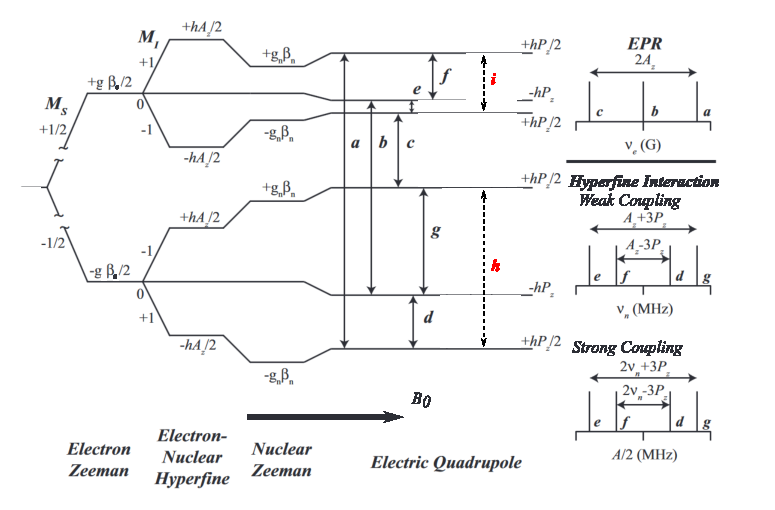
\includegraphics[width=\textwidth]{Kapitel/Ch2-Images/EnergyDiagram.eps}
 \caption[Energy diagram example with S=1/2 and I=1.]{Energy diagram example of a spin system with $S=1/2$, $I=1$, and first-order quadrupole interactions. The transitions $\mathbf{a}$, $\mathbf{b}$, and $\mathbf{c}$ are EPR transitions. The nuclear hyperfine-interaction transitions are marked as $\mathbf{d}$, $\mathbf{e}$, $\mathbf{f}$, and $\mathbf{g}$. The transitions shown as dashed lines are semi-forbidden ``double quantum'' $\Delta M_I = \pm 2$ transitions and marked in red as marked as $\mathbf{h}$ and $\mathbf{i}$. Modified with permission from Fig.~2 of Ref.~[2.\kern-0.4em\citenum{CUTSAIL20151370}].}
 \label{fig:EPREnergy}
\end{figure}

In this formulation, the static magnetic field $\mathbf{B}_0$ is assumed to be along the $z$ axis and denote the transpose of a tensor with a `T'. In this work, it is assumed that the electron Zeeman interaction is the largest interaction followed by the hyperfine interaction, nuclear Zeeman, electric quadrupole, and zero-field splitting.

\subsubsection*{Zeeman interactions}
When a static magnetic field is applied to a molecular system with angular momentum, the angular momentum aligns in such a way that a Boltzmann distribution is formed. This removes the degeneracy of the electron magnetization $\mathbf{M}_s$ manifold, splitting the energy levels, illustrated in Fig.~\ref{fig:EPREnergy} as the initial splitting. For an electron spin of $S = 1/2$, the initial energy levels are split into $\mathbf{M}_s = \ket{+\frac{1}{2}}, \ket{-\frac{1}{2}}$ for spin-up and spin-down, respectively. Both the electron $\hat{\mathcal{H}}_{ze}$ and nuclear $\hat{\mathcal{H}}_{nz}$ Zeeman interactions occur when a static magnetic field $\mathbf{B}_z$ is applied.

The electron Zeeman interaction is defined by
\begin{equation*}
    \hat{\mathcal{H}}_{ze} = \beta_e \mathbf{B}^\text{T}_z  \cdot \mathbf{g} \cdot \mathbf{S}
\end{equation*}
where $\beta_e$ is the Bohr magneton, the transpose of the static magnetic field $\mathbf{B}_z^{\text{T}}$, the vector operator $\mathbf{S} = [\mathbf{S}_x \; \mathbf{S}_y \; \mathbf{S}_z]$ is the spin angular momentum of the electron. 

A free electron in a vacuum has an isotropic spin with angular momentum. It is then the introduction of the electron with other atoms and how those atoms distribute the electron that gives rise to different components of the spin Hamiltonian.\cite{abragam2012electron,harriman1978theoretical} This ``pushing'' and ``pulling'' of the electron by spin-orbit coupling leads to anisotropic $\mathbf{g}$. The matrix $\mathbf{g}$ is what is known as the $g$-tensor and is a spatial distribution of the angular momentum of the electron. The $g$-tensor is typically made diagonal and discussed in terms of the $g_x$, $g_y$, and $g_z$ principal components, where the magnitude is denoted as $g_{iso}$. EPR resonance occurs as a result of the incident energy is matched by the energy difference of the electron Zeeman levels. 

Deviations from a free-electron can be used to obtain information on the local environment. Since these processes are non-cooperative, we can separate the free-electron from all the other contributions
\begin{equation*}
    \mathbf{g} = g_e \mathbf{1} + \Delta \mathbf{g},
\end{equation*}
where $\mathbf{1}$ is the identity matrix and $\Delta \mathbf{g}$ includes isotropic terms as well as second-order spin-orbit coupling terms. The interaction between the electron spin and the atomic orbitals of the molecule arise due to the magnetic moment of the electron. \cite{griffith1964theory} The electron Zeeman $\hat{\mathcal{H}}_{ze}$ interaction is then a perturbation of the free electron in the ground state. 

For systems when the electron interacts with intrinsic or surrounding nuclei with a nuclear spin $I_k$, the Nuclear Zeeman effect is added to $\hat{\mathcal{H}}$ as
\begin{equation*}
    \hat{\mathcal{H}}_{nz} = - \beta_n \sum_{k=1}^m g_{n,k} \mathbf{B}^\text{T}_z  \cdot \mathbf{I}_k,
\end{equation*}
where $\beta_n$ is the nuclear magneton, the transpose of the static magnetic field $\mathbf{B}_z$ is marked with a `T', the vector operator $\mathbf{I}_k = [\mathbf{I}_x \; \mathbf{I}_y \; \mathbf{I}_z]$ is the spin angular momentum of the nuclei. The summation of the nuclear contributions are represented by the index $k$ for each $m$ nucleus that interacts with the electron. Each nucleus has a distinct nuclear $g_{n,k}$-value and angular momentum $\mathbf{I}_k$ and is assumed to be isotropic. The visualization of the nuclear Zeeman effect is illustrated as a perturbation on the electron-nuclear hyperfine interaction shown in Fig.~\ref{fig:EPREnergy}.

\subsubsection*{Nuclear-Electron Interactions}
Since EPR is the measurement of how a valence electron interacts with the surrounding environment, information on the surrounding nuclei is possible if these nuclei have an inherent nuclear spin $\mathbf{I}$. Such nuclei include, for example, $^1$H, $^2$H, $^{14}$N, $^{15}$N, $^{57}$Fe, and $^{13}$C, which can be synthetically incorporated into the system to gain more information than the natural abundance of some of the atoms. \cite{Doorslaer2007,Harmer2009,CUTSAIL20151370}

\paragraph*{Hyperfine Interactions}
The hyperfine interactions are defined as the coupling between the paramagnetic site and the surrounding nuclei. This can be broken up into two distinct parts, the isotropic Fermi contact interaction, $a_{iso}$, and the electron-nucleus magnetic dipole-dipole coupling. The hyperfine interactions can be expressed as
\begin{equation}
    \hat{\mathcal{H}}_{hfi} = \mathbf{S}^{\text{T}} \cdot \mathbf{A} \cdot \mathbf{I}_k = a_{iso}\mathbf{S}^{\text{T}} \cdot \mathbf{I}_k + \mathbf{S}^{\text{T}} \cdot \mathbf{T} \cdot \mathbf{I}_k \label{eq-2:hfi}
\end{equation}
for each the interacting nuclei $k$, there exists such an interaction. The Fermi contact describes the delocalization of the electron to the surrounding nuclei. At a sufficient distance, the spacial tensor $\mathbf{T}$ can be described by
\begin{equation}
    \mathbf{T} = \frac{\mu_0}{4 \pi \hbar}\frac{1}{r^3} g_n \beta_n \beta_e g_i (3r_i r_j - \delta_{ij}) \qquad (i,j = x,y,z), \label{eq-2:hfiT}
\end{equation}
where the $x$, $y$, and $z$-components of the hyperfine tensor are treated independently. Illustrated in Fig.~\ref{fig:EPREnergy} is the nuclear-electron hyperfine interaction assuming only the isotropic component of interaction. In frozen solution, this isotropic component is broadened by the distribution of the frequency components defined by $\mathbf{T}$. Only single-crystal EPR spectroscopy can truly obtain the full hyperfine-tensor information for systems with anisotropic hyperfine interactions $\mathbf{T}$ by measuring the total hyperfine interaction $\mathbf{A}$.

\paragraph*{Electric-Nuclear Quadrupole Interactions}
The electric-nuclear quadrupole interaction only exists for nuclei with a spin $I$ greater than 1/2 and is caused by electric field gradients due to the interaction of the electron with the second moment of the nuclear angular momentum. This can be rationalized since the nuclear Zeeman interaction is assumed to be isotropic, while the second moment (gradient) is a measurement of the deviation from isotropic angular momentum. One can learn about the nature of the chemical bonding and the delocalization of the electron if the quadrupole moment $Q$ is known.\cite{quadref} 

The electric-nuclear quadrupole interaction is described by the Hamiltonian
\begin{equation}
    \hat{\mathcal{H}}_{nqi} = \mathbf{\hat{I}}^\text{T} \cdot \mathbf{P} \cdot \mathbf{\hat{I}} \label{eq-2:nqi}
\end{equation}
where
\begin{equation}
    \mathbf{P} = P_{||}   \begin{bmatrix}
   \eta_Q -1 & 0 & 0\\
     & \eta_Q -1 & 0\\
    &   & 2\\
   \end{bmatrix}
\end{equation}
and the value 
\begin{equation}
    P_{||} = \frac{3 e Q}{4I(2I-1)}\frac{\partial^2 V}{\partial z^2} = \frac{3 P_z}{2}
\end{equation}
where $\frac{\partial^2 V}{\partial z^2}$ is the electric-field gradient seen by the nucleus and $|e|Q$ describes the electric shape of the nucleus and is directly determined by the type of nucleus and, here, $\eta$ is defined as the rhombicity of the electric gradient calculated by $(Px-Py)/P_z$ when $|P_z|\geq |P_y|\geq |P_x|$. \cite{abragam2012electron,weil2007electron} The final EPR spectrum is a combination of all of these effects yielding a change in the Boltzmann population at the static magnetic field position illustrated in Fig.~\ref{fig:EPREnergy} as arrows marked $\mathbf{a}$, $\mathbf{b}$, and $\mathbf{c}$ and plotted as a transition stick diagram in the top right.

The hyperfine interactions that are measured with some double-resonance experiments are indicated in Fig.~\ref{fig:EPREnergy} as the arrows marked $\mathbf{d}$, $\mathbf{e}$, $\mathbf{f}$, and $\mathbf{g}$. However, when performing hyperfine spectroscopy the semi-forbidden ``double quantum'' (DQ) transitions need to be understood. In Fig.~\ref{fig:EPREnergy}, these transitions are shown as dashed lines and marked in red as $\mathbf{h}$ and $\mathbf{i}$. The DQ transitions are a second-order effect on the electric-nuclear quadrupole interactions and can be calculated by
\begin{equation}
\nu^{DQ}_{\alpha, \beta} = 2 \sqrt{\bigg(\nu_I \pm \frac{a}{2}\bigg)^2+\bigg(\frac{e^2 q Q}{4 h}\bigg)(3+\eta)}, \label{eq-2:doubleQ}
\end{equation}
where $a$ is the hyperfine coupling at the nuclei of interest. \cite{Doorslaer2007} This splitting further complicates the interpretation of the data. However, when measured in single crystals the double-quantum cross peaks can be used to assign nuclei throughout the rotation.

\subsubsection*{Multiple Electron Interactions}
\paragraph*{Zero-field Splitting}
For electron with spin greater than 1/2 ($S > 1/2$) or an effective spin of multiple electrons with strong coupling greater than 1/2 ($S_{eff} > 1/2$), there exists an internal interaction that splits the energy levels of the ground state with no applied external field. This interaction, named zero-field splitting, is defined as 
\begin{equation}
    \hat{\mathcal{H}}_{zfs} = \mathbf{S}^{\text{T} } \cdot \mathbf{D} \cdot \mathbf{S}
\end{equation}
where the zero-field splitting tensor $\mathbf{D}$ is a symmetric interaction from close spin-orbital coupling between two or more electrons. The zero-field splitting is especially important in molecular magnets, where it is the direct characterization of the magnetization caused by the interactions of electrons as magnetic monopoles. \cite{barra1998high} With very large values of $D$, the EPR transistion only become excited with high-field--high-frequency EPR methods. \cite{Nehrkorn13} 

\section{On the use of Magnetic Field and Flux Density}
The EPR literature uses the magnetic field $\mathbf{H}$ and magnetic flux density $\mathbf{B}$ interchangeably as ``magnetic field''. It is somewhat disingenuous to state that the relationship of the magnetic field and magnetic flux density is simply related by the free-space permeability $\mu_0$. The focus of this section is to define the usage in this dissertation by following the nomenclature of Jackson of Ref.~[2.\kern-0.4em\citenum{jackson1975classical}] so that 
\begin{equation}
    \mathbf{B} = \mu_0(\mathbf{M} + \mathbf{H}),
\end{equation}
where the SI units for $\mathbf{B}$ is measured in Tesla, while $\mathbf{H}$ is calculated in Ampere per meter. The magnetic susceptibility $\mathbf{M}$ becomes relevant when the time-varying magnetic flux density $\mathbf{B}$ is incident on a material, such as a sample. For brevity, the time-varying magnetic flux density is defined as
\begin{equation}
    \mathbf{B}_1 = \mathbf{B} e^{-i\omega t}
\end{equation}
where $\omega$ is the frequency of interest (radians per second). It is the magnetic flux density that is incident on the sample defined by the magnetic field profile of the microwave resonator. As anticipated, the magnetic susceptibility is material-specific and is proportional to the magnetic moment of the material. In a macroscopic sense, it is the perturbation of this magnetic moment that is measured in EPR. For experimental methods, this is described in detail in Section~2.5 and used extensively in the formulation of Chapter~4. The magnetic susceptibility has the units of Ampere per meter.

From Maxwell's equations, the magnetic field is calculated by the curl of the magnetic potential and, in a vacuum, describes the relationship of the applied currents to the geometry and boundary conditions. \cite{jackson1975classical} In this dissertation when a microwave resonator is discussed, it is the magnetic field profile that is calculated and plotted. However, it is the magnetic flux density that interacts with the sample and is the experimentally measurable quantity. This is because the magnetic flux density is the mechanical torque that is applied to the magnetic moment of the material. 

This distinction is constant throughout the dissertation. If the quantity is measurable and interacts with the sample, it must be described in terms of the magnetic flux density $\mathbf{B}_1$, while calculated profiles are described in terms of magnetic field $\mathbf{H}_1$.

Finally, the static magnetic field is simply referred to as $\mathbf{B}_0$ with units of miliTesla (10$^{-1}$ Gauss\footnote{In modern EPR literature the use of mT is now favored over G.}) since no time-varying magnetic susceptibility exists. A static magnetic field is the only instance where the dual ``magnetic field'' nomenclature is correct when referring to~$\mathbf{B}$.

\section{Crystal Orientations and Molecular Frames}
In this section, the basic understanding of crystal orientations and how to relate them to the EPR experiment is discussed. 

\begin{figure}[ht]
 \centering
 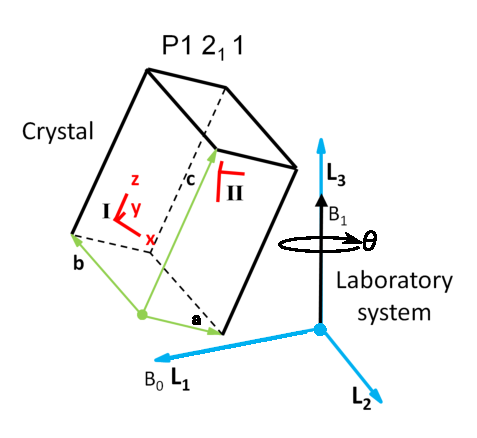
\includegraphics[width=0.75\textwidth]{Kapitel/Ch1-images/CrystalRotation.eps}
 \caption[Single crystal EPR frames.]{Relation of the Laboratory system frame $[\mathbf{L}_1\; \mathbf{L}_2\; \mathbf{L}_3]$ to the crystal frame $[\mathbf{a}\; \mathbf{b}\; \mathbf{c}]$ and the molecular frame $[\mathbf{x}\; \mathbf{y}\; \mathbf{z}]$. The molecular frame at Site I and Site II are related the crystal symmetry. The P$1\;2_1\;1$ crystal symmetry depicted here is occurs in CpI [FeFe]-hydrogenase PDB ID: 4XDC.\cite{FeFeCry} used in Chapter~6.}
 \label{fig:CrystalOrientation}
\end{figure}

\paragraph*{Laboratory System Frame} The Laboratory system frame $[\mathbf{L}_1\; \mathbf{L}_2\; \mathbf{L}_3]$ is illustrated in Fig.~\ref{fig:CrystalOrientation} as the blue coordinate system. The laboratory system frame represents the physical coordinates as it exists in the EPR laboratory. The laboratory system frame is defined with the static magnetic field (${\textbf B}_0$) oriented along the L$_1$-axis, while the microwave magnetic flux density (${\textbf B}_1$) is along the L$_3$-axis. 

\paragraph*{Crystal Frame} The crystal frame $[\mathbf{a}\; \mathbf{b}\; \mathbf{c}]$ is defined with respect to the laboratory frame. When the crystal is inserted into the resonator, the crystal orientation is typically unknown. The crystal frame rotation can be defined by a set of Euler angles. Herein the nomenclature of the EasySpin simulation package. \cite{STOLL200642} The three Euler angles ($\alpha$, $\beta$, $\gamma$) define the rotation around defined axes of the current frame. The first angle $\alpha$ is a rotation around the $z$-component, defined by
\begin{equation}
    Rot_z[\theta] = \begin{bmatrix}
   Cos[\theta] & -Sin[\theta] & 0\\
    Sin[\theta] & Cos[\theta] & 0\\
    0 &  0 & 1
   \end{bmatrix}
\end{equation}
and the second angle $\beta$ is a rotation around the new $y$-component denoted $y'$, defined by
\begin{equation}
    Rot_y[\theta] = \begin{bmatrix}
   Cos[\theta] & 0 & Sin[\theta]\\
     & 1 & 0\\
    -Sin[\theta] &  0 & Cos[\theta]
   \end{bmatrix}
\end{equation}
and finally the angle $\gamma$ is another rotation around the new $z$-component denoted $z''$. This is aptly named the zyz convention. This transformation can be performed directly by calculating the rotation matrix, such that
\begin{equation}
    Rot_{zyz}[\alpha, \beta, \gamma] = Rot_{z''}[\gamma] \cdot Rot_{y'}[\beta] \cdot Rot_z[\alpha],
\end{equation}
and applying it to the coordinates of the crystal frame
\begin{equation}
 \begin{bmatrix}
  \tilde{x}_\text{L1} & \tilde{x}_\text{L2} & \tilde{x}_\text{L3} \\
  \tilde{y}_\text{L1} & \tilde{y}_\text{L2} & \tilde{y}_\text{L3} \\
  \tilde{z}_\text{L1} & \tilde{z}_\text{L2} & \tilde{z}_\text{L3} 
  \end{bmatrix} = Rot_{zyz}[\alpha, \beta, \gamma] \cdot \begin{bmatrix}
  a_1 & a_2 & a_3 \\
  b_1 & b_2 & b_3 \\
  c_1 & c_2 & c_3 
  \end{bmatrix}\label{eqn:rotate}.
\end{equation}
Using Eqn.~\ref{eqn:rotate}, the crystal frame $[\mathbf{a}\; \mathbf{b}\; \mathbf{c}]$ is rotated with respect to the laboratory frame $[\mathbf{L}_1\; \mathbf{L}_2\; \mathbf{L}_3]$. 

\paragraph*{Molecular Frame} The molecular frame relates the measured atomic structure from X-ray crystallography diffraction experiments to the crystal frame. In Fig.~\ref{fig:CrystalOrientation}, the molecular frame is represented by the red coordinate systems sites labeled I and II (Site I and Site II). This frame is arbitrary and is defined by the spectroscopist. The frame consists of a rectangular coordinate system and is defined with a set origin. For EPR, the origin is chosen to be where a majority of the spin density is expected to reside. This can be aided by quantum chemical calculations. The illustration of Fig.~\ref{fig:CrystalOrientation} is depicting P$1\,2_1\,1$ crystal symmetry where a second axis (Site II) is defined by a rotation and translation in the direction of the $\mathbf{b}$-axis, see below. 

During crystallization, an asymmetric unit may form. An asymmetric unit is where two or more enzymes bind together to form a sub-unit cell that is rotated and translated, as a whole, within the crystal symmetry. These sub-units must be consistent within the entire volume to obtain good X-ray crystallography diffraction data. Since each one of the enzymes produces an EPR signal the asymmetric unit must be taken into account. This is done by defining a second (or more) molecular frame per site. Again, the X-ray crystallography diffraction data provides the sub-unit geometry and a rectangular coordinate system is defined. 

Every frame that gives rise to the simulated EPR signal is derived from the molecular frame. 

\paragraph{g-Tensor Frame} The $g$-tensor frame is an approximation in rectangular coordinate to the relationship of the $g_x$, $g_y$, and $g_z$ components of the $g$-tensor. This rectangular coordinate system is defined as a rotation from the chosen molecular frame. For this reason, it is important to choose the molecular frame to have an origin where the majority of spin density resides. In EasySpin, the $g$-tensor is represented as Euler angles or rotation matrices.

\paragraph{A-Tensor and Quadrupole Frames} The A-tensor frame is, in rectangular coordinates, the relationship of the total hyperfine-interaction A$_x$, A$_y$, and A$_z$ components to the molecular frame. While the quadrupole frame represents the relationship of $P_{||}$ to the molecular frame. 

Similar to the $g$-tensor, they are defined as a rotation from the chosen molecular frame. In EasySpin, the A-tensor and quadrupole frames can be represented as Euler angles or rotation matrices. 

\paragraph*{Crystal Symmetry} In general, the crystal symmetry can be described by Euler angle rotation and a spacial translation. \cite{hovmoller1981rotation} From the vector $\mathbf{x}$ a copy to the ``equivalent position'' $\mathbf{\tilde{x}}$ is formed at the rotated $R_{yxy}[\alpha,\beta,\gamma]$ and translated $\mathbf{t}$ position in the crystal, described by
\begin{equation}
\mathbf{\tilde{x}} = R_{yxy}[\alpha,\beta,\gamma] \cdot \mathbf{x} + \mathbf{t}.
\end{equation}

For the P$1\,2_1\,1$ symmetry, it has a $[\tilde{a},\;\tilde{b},\;\tilde{c}]$ of $[-a,\;b+1/2,\;-c]$. This can be performed with a rotation matrix and translation defined by 
\begin{equation}
     \begin{bmatrix}
  \tilde{a} \\
  \tilde{b} \\
  \tilde{c} 
  \end{bmatrix} = \begin{bmatrix}
   -1 & 0 & 0\\
    0 & 1 & 0\\
    0 &  0 & -1\\
   \end{bmatrix} \cdot      \begin{bmatrix}
  a \\
  b \\
  c 
  \end{bmatrix} + \begin{bmatrix}
  0 \\
  1/2 \\
  0 
  \end{bmatrix},
\end{equation}
and places the enzyme at Site II. The crystal symmetry can be taken into account in the EasySpin simulations where the duplication and rotation of the molecular frame is automatically generated. 

For the case of the CpI [FeFe]-hydrogenase from PDB ID 4XDC,\cite{FeFeCry} the enzymes crystallize into a P$1\,2_1\,1$ symmetry and each site contains an asymmetric sub-unit consisting of two enzymes. Two molecular frames are defined and the P$1\,2_1\,1$ crystal symmetry duplicates the asymmetric unit from Site I to Site II, illustrated in Fig.~\ref{fig:CrystalOrientation}. For EPR, each molecular frame per asymmetric unit gives rise to an EPR signal. Therefore, for CpI [FeFe]-hydrogenase from PDB ID 4XDC, there will exist four total EPR signals per unit cell, see Chapter~6.

The quality of the protein single-crystal is important to both the characteristics of the acquired EPR signal and the consistency of the fit for the molecular frame. Crystals grown from proteins can suffer from mosaicity, which is a crystalline state where a single crystal may be broken into blocks of unit cells that are disassociating from the whole crystal. However, mosaicity is only a perturbation on the whole crystal and is not yet poly-crystalline, where the unit cells have formed a semi-random orientation. 

Mosaicity can affect both the X-ray crystallography diffraction data and the EPR signal. Such mosaicity effects are apparent in the X-ray crystallography diffraction data by limits imposed on the spatial resolution of the electron density map. \cite{blundell1976protein} Depending on the severity, the EPR signal will be broadened which reduces the overall signal-to-noise ratio. These effects may be reduced by annealing techniques. \cite{Kriminskien0056}

\begin{figure}[htb]
 \centering
 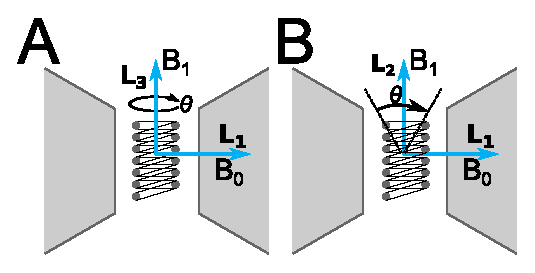
\includegraphics[width=0.5\textwidth]{Kapitel/Ch2-Images/RotateMeLeftRight.eps}
 \caption[Rotation Planes of micro-Helix.]{Shown are the two rotation planes available for crystal rotation in the self-resonant micro-helix of Chapter~5. A) A full 180 degree rotation is available when the ${\textbf B}_1$ is along the L$_3$-axis. B) A second plane is available when the ${\textbf B}_1$ is along the L$_2$-axis. A rotation in this plane is limited by a sinusoidal dependence of the EPR signal. }
 \label{fig:RotateMe}
\end{figure}

\paragraph*{Crystal Rotation} To obtain a magnetic resonance rotation pattern, the crystal must be rotated with respect $\mathbf{B}_0$, illustrated in Fig.~\ref{fig:RotateMe}A. This is currently performed by rotating the entire resonator probe around the L$_3$-axis. If a second plane is needed, the angle can be modified by orientating the $\mathbf{B}_1$ along the L$_2$-axis, illustrated in Fig.~\ref{fig:RotateMe}B by using a 90$^{\circ}$ bend. This secondary plane of rotation is limited since the EPR signal has a sinusoidal dependence is reduced as $\mathbf{B}_1$ becomes parallel to $\mathbf{B}_0$. With a good signal-to-noise ratio, EPR can be collected over a 120 degree rotation.

\section{Finite-element modeling Simulations}
Commercially available electromagnetic finite-modeling software provides a suite in which boundary conditions, sources, and dielectric properties are combined to solve Maxwell's equations in a CAD-like environment. In this dissertation, finite-element modeling is used to design, understand, and optimize microwave resonators. Here, an introduction to Ansys Electromagnetics Suite (Pittsburgh, PA, USA; version 19.4; High Frequency Structure Simulator (HFSS)) and a practical exercise will be developed. 

Ansys HFSS employs ``driven-mode'' and ``eigenmode'' solving domains. The ``eigenmode'' solver uses Maxwell's equations in their variational form to find the lowest energy states of a structure given its boundary conditions and electromagnetic material properties. \cite{sadiku2000numerical,jin2015finite} This lowest energy state, or eigenvalue, is then used to calculate the eigenvectors of the structure, yielding a wave solution. The eigenvalue problem assumes that both the differential equations and the boundary conditions are homogeneous. There is no source exciting the mode of interest. This becomes very important in geometries where the modes of the system are not known. In Ansys Electronics Desktop, solutions are normalized by the electric field (1~V/m) or to the stored electric energy.

The ``driven-mode'' solves the non-homogeneous Maxwell's equations. Practically, one must devise a coupling system in ``driven-mode'' and, in this work, impedance matching considerations are implemented to maximize power transfer to the resonator. The ``driven-mode'' provides outputs similar to a vector network analyzer and is typically normalized to an input power of 1~W. 

\paragraph*{Signal Calculations and Resonator Comparisons.}
A method to obtain the EPR signal has been formulated and is reproduced here. \cite{misrabook} This method uses the fields calculated in Ansys HFSS, accessed by the ``Field Calculator'', to determine a normalized EPR signal under saturating or nonsaturating conditions. This calculation can be performed using eigenmode or driven-mode methods and the scripts for Ansys HFSS are found in Appendix~B.\footnote{All codes and HFSS files can be found at https://github.com/jsidabras/HFSSTutorial/.} 

\begin{wrapfigure}{R}{4cm}
\centering
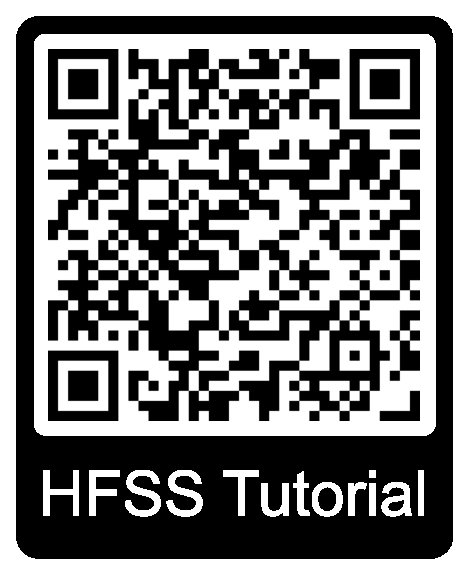
\includegraphics[width=4cm]{Kapitel/Appendix/HFSSTutQR.eps}
\end{wrapfigure}

For a matched reflection cavity and a voltage-sensitive detector, Feher expressed the microwave EPR signal as
\begin{equation}
    S \propto \chi'' \eta Q P^{1/2} \qquad [\text{V}],\label{ch2-fehereq}
\end{equation}
where $\chi''$ is the imaginary part of the magnetic susceptibility which represents the magnitude of the absorption spectrum, $\eta$ is the filling factor, $Q$ is the unloaded $Q_0$-value with a sample, and $P$ is the incident microwave power.  \cite{FeherSignal} The signal is proportional to volts when the system is critically coupled and calculated at microwave resonance. When comparing resonators, the sample has the same concentration for an arbitrary volume and, as such, the magnetic susceptibility $\chi''$ is simply proportional to frequency. This assumption is used to incorporate the Boltzmann factor to resonator comparisons (i.e. temperature or frequency differences).

The $Q$-value of the system can be calculated by the ratio of the stored energy per cycle and the power losses. Such that
\begin{equation}
    Q = \frac{\omega U_m}{P_l},\label{ch2-Qval}
\end{equation}
where $\omega$ is the microwave resonance frequency in radians per second, $U_m$ is the stored magnetic energy, and $P_l$ is the power losses in the cavity walls and sample. At resonance, the magnetic and electric stored energy are equal. \cite{ramo1984fields} However, the magnetic stored energy is chosen for simplicity when dealing with a geometry where there are different dielectric volumes. Electric stored energy includes the relative permittivity $\epsilon_r$ accounted for in each volume, while magnetic stored energy includes the relative permeability $\mu_r$. In this formulation, the relative permeability is equal to unity and only the free-space permeability $\mu_0$ is needed. Therefore the magnetic stored energy is
\begin{equation}
    U_m = \frac{\mu_0}{2} \int \mathbf{H}_1\cdot\mathbf{H}_1^* dV \qquad [\text{W}],
\end{equation}
where ${\textbf H}_1$ is the microwave magnetic field in all space ($V$) including the sample.

The filling factor is defined as the ratio of the magnetic flux density energy in the sample that gives rise to an EPR signal to the microwave magnetic field energy in all space. This can be calculated as
\begin{equation}
 \eta = \frac{\int {\mathbf B}_{1r} \cdot {\mathbf B}_{1r}^* dV_s}{\mu_0 \int {\mathbf H}_1 \cdot {\mathbf H}_1^* dV}, \label{eq-2:filling}
\end{equation}
where ${\textbf B}_{1r}$ is one component of the clockwise (or counter clockwise) rotational component of the linearly polarized flux density ${\textbf B}_1$ perpendicular to the static magnetic field in the sample volume ($V_s$). \cite{jackson1975classical} In magnetic resonance, the spin system is coupled to either the right-handed or left-handed (clockwise or counter clockwise) polarization of the magnetic flux density. \cite{abragam1961}

A linearly polarized wave can be decomposed into two in-phase circular components. From Ref.~[2.\kern-0.4em\citenum{jackson1975classical}], an expression for the right-handed ($+$) or left-handed ($-$) component of the magnetic flux density can be derived, such that
\begin{equation}
    \mathbf{B}_{\pm} =  \mathbf{B}\cdot\frac{\mathbf{\hat{y}} \pm i\mathbf{\hat{z}}}{\sqrt{2}} \qquad \text{[T]}, \label{circpoleHpm}
\end{equation}
where the static magnetic field B$_0$ is in the $\mathbf{\hat{x}}$ direction. In cavity resonators, where the microwave magnetic field is well defined, the left- and right-handed components are equal. However, open structures and systems with multiple wavelengths within the sample could exhibit elliptical polarization. This results in different magnitudes and field profiles for the two components. The component of the magnetic flux density that interacts with the sample during resonance is the amplitude of Eqn.~\ref{circpoleHpm}, therefore, the magnitude of the microwave magnetic flux density in the (right-handed) rotating frame is the amplitude of Re($\mathbf{B}_+\epsilon_+e^{-iwt}$) such that
\begin{equation}
    \mathbf{B}_{1r} =  \frac{|\mathbf{B}_{+}|}{\sqrt{2}} \qquad \text{[T]}. \label{circpoleH}
\end{equation}
Herein, this formulation was only applied to systems that exhibit linear polarization in the sample (Chapter~3 and 5) and other methods were relied upon to approximate the EPR signal in cases where multiple wavelengths are involved (Chapter~4).

The power loss in the system is broken up into two distinct types: dielectric losses and Ohmic losses on the surfaces of conductors. For a bulk conductor, the power dissipated on the surface can be calculated as
\begin{equation}
    P_{lw} = \frac{R_s}{2}\int \mathbf{\hat{n}}\times\mathbf{H}\cdot\mathbf{H}^* dS_w \qquad [\text{W}]
\end{equation}
where $\mathbf{\hat{n}}$ is normal to the conductor surface ($S_w$). The resistance of the surface is calculated by the real part of the surface impedance, defined as
\begin{equation}
    Z_s = \sqrt{\frac{\omega \mu_0}{2 \sigma}}(1-i)
\end{equation}
where $\sigma$ is the conductivity of the metal surface. The power dissipated in a dielectric can be calculated by
\begin{equation}
    P_{ld} = \frac{\omega \epsilon_0 \epsilon_r''}{2}\int \mathbf{E} \cdot \mathbf{E}^* dV_d \qquad [\text{W}],
\end{equation}
where the imaginary part of the dielectric permittivity ($\epsilon_r = \epsilon_r' - i \epsilon_r''$) is integrated over the dielectric volume $V_d$. \cite{jackson1975classical,harrington1961time} The total power loss of the system is the summation of all the power losses of the conductors and $n$ is the number of dielectrics which may include the sample, sample tube, and other plastics and ceramics such that
\begin{equation}
    P_l = P_{lw} + \sum_{i=1}^n P_{ld_i} \qquad \text{[W].}
\end{equation}
The power loss in the system for the sample, resonator walls, and sample holder end sections is defined as $P_s$, $P_w$, and $P_e$, respectively, in the scripts of Appendix~B. The calculations for $P_s$ and $P_e$ rely on the constants \textit{ImDiSam} and \textit{ImDiHold} which are set to the imaginary part of the relative permittivity constant $\epsilon_r''$.

From Eqn.~\ref{ch2-fehereq} the signal can be calculated by substituting the appropriate equations. Two EPR signal conditions can be calculated: signal unsaturable (Su; Unsat.) and signal saturable (Ss; Sat.). In continuous-wave experiments, signal unsaturable is defined as the EPR signal at constant incident power, while signal saturable is defined as the EPR signal at a constant magnetic flux density at the sample. A saturable sample can be calculated by normalizing to the magnetic flux density and computing
\begin{equation}
    S_s = \frac{\chi'' \omega}{10^4 P_l^{1/2} \text{Max}|\mathbf{B}_{1r}|} \int \mathbf{B}_{1r} \cdot \mathbf{B}_{1r}^* dV_s \qquad \text{[V]}. \label{ch2-eq:ss}
\end{equation}{}
The unsaturable sample can be calculated by normalizing to the power and computing
\begin{equation}
    S_u = \frac{\chi'' \omega}{P_l} \int \mathbf{B}_{1r} \cdot \mathbf{B}_{1r}^* dV_s \qquad  \text{[V]}. \label{ch2-eq:su}
\end{equation}{}
The efficiency parameter $\Lambda_{max}$, as introduced by Hyde {\em et al.} \cite{hydehoff}, is defined as
\begin{equation}
    \Lambda_{max} = \frac{1}{10}\frac{\text{Max}|\mathbf{B}_{1r}|}{P_l^{1/2}} \quad \text{[mT/W}^{1/2}], \label{ch2-eq:lammax}
\end{equation}
where Max$|\mathbf{B}_{1r}|$ is the maximum magnitude of $\mathbf{B}_{1r}$ in the sample (typically in the center of the cavity) and is assumed to be uniform over the sample volume. \cite{hydehoff} The scalar converts Gauss into milliTesla. 

To better assess the resonator efficiency when $\mathbf{B}_{1r}$ is not uniform, an average over the sample volume is calculated, 
\begin{equation}
    \Lambda_{ave} = \frac{1}{10}\frac{\int \sqrt{\mathbf{B}_{1r} \cdot \mathbf{B}_{1r}^*} dV_s}{P_l^{1/2} V_t} \quad [mT/W^{1/2}], \label{ch2-eq:lamave}
\end{equation}
where $V_t$ is the total volume of the sample. The average resonator efficiency, which takes into account the $\mathbf{B}_{1r}$ profile along the sample volume, is the measurable value when a nutation experiment is performed.

Finally, the $\Lambda_{ave}$-to-$\Lambda_{max}$ ratio can be used as a metric to quantify the uniformity of the resonator. \cite{UFLGR2017} The B$_1$ profile uniformity (in percent) is defined by 
\begin{equation}
    \Delta B_1 = \frac{\left| \Lambda_{max} - \Lambda_{ave} \right|}{\Lambda_{max}} \times 100\%.
\end{equation}

\section{Experimental Measurement of EPR Spectra}
The EPR experiments performed in this work are as follows:

\subsubsection*{Continuous-wave EPR.}
The continuous-wave (CW) EPR experiment measures the sample using a constant microwave B$_1$ at a fixed frequency ($\omega$) incident on the sample and slowly sweeping B$_0$. As the resonance condition is met, when the incident energy ($E =\hbar \omega$) is equal to the Zeeman splitting, the angular momentum is perturbed and an absorption of the energy is recorded.\footnote{In order to relate this to a real spectrum, we say this happens ``in the neighborhood'' of resonance $\omega_0$ and assume the linewidth is caused by a general broadening from the spin-lattice relaxation time. This assumes homogeneous broadening, as opposed to inhomogeneous broadening. For example, broadening from hyperfine interactions, environmental deviations, etc.}   

At the macro-scale view, the absorption of the microwaves cause a change in the permeability of the sample through a perturbation of the magnetic susceptibility M,
\begin{equation}
    \mu_r(\omega) = \mu_0 (1+M) = \mu_0 (1+ 4 \pi \eta \chi(\omega)), \label{eq-2:permea}
\end{equation} 
where $\eta$ is the filling factor from Eqn.~\ref{eq-2:filling} which describes the flux-linkage efficiency between the applied microwave magnetic field and the sample and $\chi(\omega)$ is the complex time-dependant magnetic susceptibility. For a simple Lorenzian-shaped spectrum, the magnetic susceptibility is 
\begin{equation}
      \chi(\omega) = \frac{(\omega_0 - \omega) T_1 }{1+(\omega_0 - \omega)T_2^2+\gamma^2 H_{1r} T_1 T_2}- i \frac{1}{1+(\omega_0 - \omega)T_2^2+\gamma^2 H_{1r} T_1 T_2}, \label{eq-2:chi}
\end{equation}
where $T_1$ and $T_2$ are the spin-spin and spin-lattice relaxation times, respectively, $\omega_0$ is the frequency of resonance as $\omega$ is swept, $H_{1r}$ is the microwave magnetic field perpendicular to $\vectu{B}{0}$ (Eqn.~\ref{circpoleH} and $\gamma$ is an isotropic gyromagnetic ratio. \cite{abragam1961}

Assuming a simple lumped-circuit resonance consisting of an inductor $L_R$ (which contains the sample) in series with a resistor $R_R$ in parallel with a capacitance $C_R$. The capacitor is chosen so the tank circuit resonates at the frequency $\omega_R^2 L_R C_R = 1$. The detector is placed across the capacitor, measuring the voltage. 

The inductance can be described by
\begin{equation}
    L_R = \mu_r L_0 = \mu_0 (1 + M)L_0 = \mu_0 (1 + 4 \pi \eta \chi)L_0,
\end{equation}
where the permeability of the sample consists of the freespace $\mu_0$ and $4\pi\chi$ is the magnetic susceptibility $M$, modified by the filling factor $\eta$. \cite{ramo1984fields} Although $\chi$ is a function of the incident microwave frequency $\chi(\omega)$, it is omitted for brevity. The resonant tank-circuit resistance and inductance can be further simplified such that
\begin{equation}
    R_R + i \omega L_R = (R_R + 4\pi \omega L_0 \eta \chi'') + i (1+4\pi\eta\chi')\omega L_0
\end{equation}
where $\omega$ is the frequency of operation and resonance occurs in the neighborhood of $(\omega_0-\omega)$. \cite{schumacher1970introduction} The change in magnetic permeability within a resonator is small compared to the microwave inductance and causes only a perturbation in the operating frequency (dispersion; $\chi'$) and losses (absorption; $\chi''$). The resonator impedance is matched to the bridge, called ``critical coupling'', where the phase of the incoming standing-wave voltage cancels the outgoing reflections. At critical coupling, no voltage is detected at the diode. However, in the neighborhood of resonance, the change in the tank-circuit resistance is directly measured as a change in the reflection coefficient. 

In the CW experiment, the static magnetic field is modulated by $B_0 + B_m Cos[2\pi f_m t]$, typically at a modulation frequency $f_m$ of 100~kHz, and is collected using a phase-sensitive detector. \cite{weil2007electron} If the modulation is small, the signal is derivative-like. \cite{Hyde1990pseudo} As the modulation amplitude $B_m$ is increased, the signal increases proportionally until the modulation amplitude approaches the intrinsic line-width of the sample where a broadening occurs. Choosing between signal and signal purity is known as the line-height--line-width compromise and is discussed in Ref.~[2.\kern-0.4em\citenum{eaton2010quantitative}]. 

The modulated reflection coefficient changes are recorded on a detector diode connected to the phase-sensitive detector. When the frequency is held constant, as is typically done with automatic frequency control (AFC), an absorption spectrum is obtained. \cite{poole1967electron} A dispersion signal can be obtained by the frequency control feedback voltage or directly detected by a quadrature microwave channel. Continuous-wave is the standard EPR experiment. 

\subsubsection*{Non-adiabatic and Adiabatic Rapid Scan.}
With modern digital signal processing and fast analog-to-digital converters, the CW experiment has recently been improved upon. The non-adiabatic rapid scan (NARS) \cite{KITTELL2011228, KITTELL201251, KITTELL201568, Hyde2013MDIFF, YU201558} and adiabatic rapid scan (RS) \cite{JOSHI200544,TSEITLIN200948, MITCHELL2012221, RScompare,MOSER2017} methods collect real and imaginary EPR spectra (pure-absorption and pure-dispersion) using magnetic field ($\mathbf{B}_0 + \mathbf{B}_m $) or microwave frequency sweeps without the need for a phase-sensitive detector. Both rapid scan methods produce data that can be post-processed with pseudo-modulation to compare to the conventional first-derivative EPR spectrum using a moving difference (MDIFF) pseudo-modulation. \cite{Hyde2013MDIFF} The non-adiabatic rapid scan (NARS) experiment uses a static field sweep fast enough to overcome $1/f$ noise but remains in thermal equilibrium, while adiabatic rapid scan sweeps the static field fast enough to cause passage. \cite{Weger1960} 

Specifically, the rapid passage regime satisfies the equation
\begin{equation}
    \frac{|\mathbf{B}_{1r}|}{d B_0/dt} \ll \sqrt{T_1 T_2}
\end{equation}
where the magnitude of the magnitude microwave magnetic field $\mathbf{B}_{1r}$, as previously defined in Eqn.~\ref{circpoleH}, and the change in static magnetic field B$_0$ must be much less than the product of the spin-lattice relaxation time $T_1$ and spin-spin relaxation time $T_2$. The adiabatic regime is defined as 
\begin{equation}
    \gamma |\mathbf{B}_{1r}|^2 \gg \frac{d B_0}{dt},
\end{equation}
where $\gamma$ is the the gyromagnetic ratio in MHz/G. Conversely, the non-adiabatic regime is defined as
\begin{equation}
    \gamma |\mathbf{B}_{1r}|^2 \ll \frac{d B_0}{dt}.
\end{equation}
These conditions produce passage. \cite{Weger1960}

The advantage of the non-adiabatic rapid scan experiment is the signal-to-noise improvement of collecting pure-absorption EPR spectra, while adiabatic rapid scan can further improve the continuous-wave and NARS experiment by changing the effective microwave magnetic field at the sample. This allows for an increase of microwave power, and thus, an increase in EPR signal for saturable signals. \cite{JOSHI200544} It should be noted that the excitation of a spin packet goes through a continuum of passage from the steady-state CW experiment to the non-adiabatic rapid scan to adiabatic rapid scan, and finally to the free-induction decay pulse. 

While the non-adiabatic rapid scan method can be implemented on commercial pulse bridges with no hardware changes, it does require some technical expertise. \cite{MOSER2017} However, to perform adiabatic rapid scan experiments on protein samples, custom current drivers are needed to increase the swept field amplitude. For simplicity, in this work, only the non-adiabatic rapid scan experiment has been implemented.

\subsubsection*{Electron Spin Echo Pulse.}
The field-swept two-pulse electron spin-echo (ESE) experiment uses a ${\pi/2\!-\!\tau\!-\!\pi}$ pulse sequence. A $\pi/2$-pulse is defined as enough microwave power to tip the magnetization of a spin packet into the M$_x$-M$_y$ plane. Such a pulse is applied Over a time $\tau$, the magnetization dephases into the $x$-$y$-plane, where an applied $\pi$-pulse inverts the magnetization. After $\tau$ seconds the spin packet becomes coherent and an echo is formed. The echo is recorded, where the intensity is a function of the magnetic susceptibility absorption $\chi''$ (Eqn.~\ref{eq-2:chi}) interacting with the resonator. The echo is proportional to the absorption of the spins at a single static field position. The static field is stepped and a whole spectrum is acquired. \cite{schweiger2001principles} For systems with little nuclei interaction, the ESE experiment will mimic the pure absorption spectrum of the CW experiment. This is the standard pulse sequence to collect an EPR spectrum, and the pulse sequence is illustrated in Fig.~\ref{fig:EPRpulse}.

\begin{figure}[ht]
 \centering
 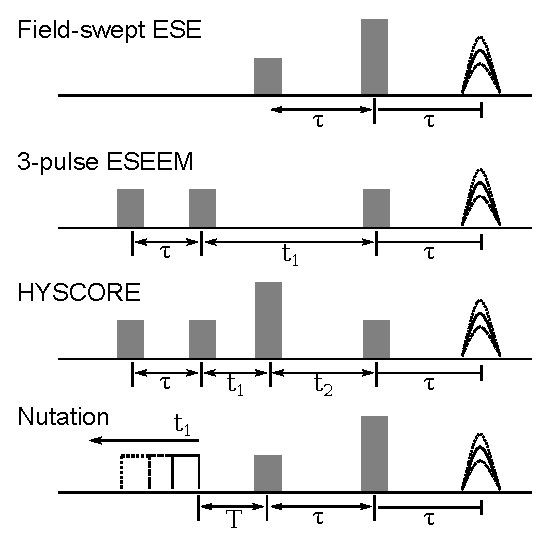
\includegraphics{Kapitel/Ch1-images/PulseExperiments.eps}
 \caption[Pulse EPR sequences.]{The pulse EPR sequences used in this work. Field-swept electron spin echo (ESE) is performed over a series of field steps, recording the entire spectrum. Electron Spin Echo Envelope Modulation (ESEEM) and Hyperfine Sub-level Correlation (HYSCORE) are performed at a single field position. The nutation experiment is used in this work to determine the efficiency parameter $\Lambda_{ave}$. }
 \label{fig:EPRpulse}
\end{figure}

Specifically, the signal from a microwave pulse is derived from the reciprocity principle of electromagnetics. \cite{HOULT2011329} The initial magnitude of the magnetization can be described as $\mathbf{M} = M_0 \mathbf{B}_z$, where $M_0$ is the dc bulk magnetization. When $\mathbf{B}_{1r}$ is applied, the bulk magnetization takes the form of the magnetic susceptibility of Eqn.~\ref{eq-2:chi}. If the excitation coil is the same as the pickup coil, after a $\pi/2$-pulse is applied, and electromotive force (emf) is induced on the coil such that 
\begin{equation}
    \xi = - \int \frac{\partial \mathbf{B}_{1r} \cdot \mathbf{M}}{\partial t} dV_s,
\end{equation}
which is transferred to a voltage across the tank-circuit capacitance. The voltage, assuming a homogeneous $\mathbf{B}_{1r}$ and a unit volume, is such that
\begin{equation}
    V_0 = - 4\pi \eta \int \frac{\partial \mathbf{B}_{1r} \cdot \mathbf{M}}{\partial t} dV_s = - 4 \pi \eta \frac{\partial \phi}{\partial t},
\end{equation}
where $\partial \phi/\partial t$ is the time-varying magnetic flux, which includes the permeability defined in Eqn.~\ref{eq-2:permea}. \cite{schumacher1970introduction,slichter1978principles,HOULT2011329} The final output to the receiver is multiplied by the $Q$-value of the tank circuit, which transforms the voltage proportional to the stored energy of the circuit. \cite{ramo1984fields} The formulation of $V_0 Q$ can be related directly to the parameters defined by Feher in Eqn.~\ref{ch2-fehereq}, where the applied microwave magnetic field is held constant in order to provide a $\pi/2$-pulse, as defined by the saturable signal conditions of Eqn.~\ref{ch2-eq:ss}.

The voltage $V_0$ decays exponentially with the spin-lattice relaxation time $T_2$ and, within the decay envelope, exists the magnetization dephasing from the $x$-$y$-plane. The signal directly after a $\pi/2$-pulse is known as the free induction decay (FID) and it is this dephasing that is refocused after time $\tau$ to form the echo in the ESE experiment. Therefore, the experimental parameter $\tau$ must be chosen to allow for sufficient ring-down of the tank-circuit, but not so long as the signal $V_0$ has decayed beyond detection.

\subsubsection*{ESEEM and HYSCORE.}
The Electron spin echo envelope modulation (ESEEM) experiment has a  pulse sequence of ${\pi/2\!-\!\tau\!-\!\pi/2\!-\!t_1\!-\!\pi/2}$. The three-pulse variation of ESEEM (3P-ESEEM) puls sequence is illustrated in Fig.~\ref{fig:EPRpulse}. ESEEM is capable of resolving hyperfine and quadrupole interactions of the electron to neighboring nuclei. It is complementary to electron-nuclear double resonance experiments (ENDOR). \cite{schweiger2001principles,Doorslaer2007,Harmer2009,CUTSAIL20151370}

The 3P-ESEEM signal used in this work arises from the semi-forbidden transitions between the different $M_s$ manifolds ($\pm \ket{\frac{1}{2}}$; Fig.~\ref{fig:EPREnergy}), but within the same $M_I$ manifold. This nuclear coherence mixing is directly probed by the dephasing that is occurring at time $\tau$ which is allowed to mix for time $t_1$. 

Unlike the two-pulse ESEEM signal, the 3P-ESEEM does not obtain the sum and differences of the modulating frequencies, potentially simplifying analysis. However, a drawback of the 3P-ESEEM method is the dependence of the signal on the $\tau$ chosen. Known as ``$\tau$-suppression'' occurs because of the time at which the coherence mixing $\pi/2$-pulse starts could be at a null of the nuclear modulation frequency. \cite{schweiger2001principles} This effect can be minimized by summing a series of 3P-ESEEM measurements at different $\tau$ values.

Two regimes of hyperfine coupling exist, denoted as strong $a_{iso}/2 < \nu_n$ and weak $a_{iso}/2 > \nu_n$ coupling, depicted in the bottom-right inset of Fig.~\ref{fig:EPREnergy}. The modulating resonance frequency $\nu_n$ is related to the nuclei by the nuclear Zeeman energy $-g_n \beta_n B_0/\hbar$. The tensor information is directly observed from the summation of the hyperfine and quadrupole interactions of Eqns.~\ref{eq-2:hfi} and \ref{eq-2:nqi}. Using an ESEEM experiments, the modulation frequencies $2\nu_n \pm 3P_z$ for strong coupling and $a_{iso} \pm 3P_z$ for weak coupling (Fig.~\ref{fig:EPREnergy} $\mathbf{d}$, $\mathbf{e}$, $\mathbf{f}$, $\mathbf{g}$) are directly observed. In addition, the double-quantum peaks (Fig.~\ref{fig:EPREnergy} $\mathbf{h}$, $\mathbf{i}$) are observed at the frequencies $\nu^DQ_{\alpha,\beta}$ described by Eqn.~\ref{eq-2:doubleQ}. The modulation depth observed in the time-domain trace is dictated by
\begin{equation}
    k(\theta) = \text{Sin}^2(2\theta) = \bigg(\frac{B_\theta}{\nu_I}{\nu_\alpha \nu_\beta}\bigg)^2
\end{equation}
where $\theta$ is the angle between the non-isotropic electron-nuclear hyperfine tensor $\mathbf{T}$ of Eqn.~\ref{eq-2:hfiT} and the static magnetic field $\mathbf{B}_z$. When either $\mathbf{T}$ is zero or $\mathbf{B}_z$ is aligned with a principal axis, the modulation depth is reduced to zero.

The hyperfine sublevel correlation (HYSCORE) experiments add an additional pulse to the 3-Pulse ESEEM. A  ${\pi/2\!-\!\tau\!-\!\pi/2\!-\!t_1\!-\!\pi\!-\!t_2\!-\!\pi/2}$ pulse sequence results in an echo $\tau$ seconds after the last $\pi/2$ pulse. The values for $t_1$ and $t_2$ are swept to form a 2D experiment at a fixed static magnetic field position. The HYSCORE experiment allows for the separation of overlapping modulation frequencies found in large anisotropic hyperfine systems. Additionally, HYSCORE separates the strong $a_{iso}/2 < \nu_n$ and weak $a_{iso}/2 > \nu_n$ coupling regimes into the ($-$,$+$) quadrant and ($+$,$+$), respectively. The use of HYSCORE allows for a visual representation of the different modulating frequencies such that the $\nu_n$ or $a_{iso}/2$ can be read directly from the graph. 

Although HYSCORE is a useful tool for visualization and human-aided analysis, a set of ESEEM spectra are typically simulated for fitting and following orientation dependant single crystal data to obtain the full hyperfine-tensor. \cite{Shane1994SingleCrystalESEEM}

\subsubsection*{Nutation.}
The nutation experiment is performed at a field position of maximum EPR signal and a perturbation pulse is added to the electron spin-echo experiment such that a pulse sequence of ${t_1\text{-pulse}\!-\!\text{T}\!-\!\pi/2\!-\!\tau\!-\!\pi}$ if formed. The $t_1$-pulse is varied resulting in a perturbation on the electron spin echo experiment at a fixed field. The variation is a function of the tip angle of the spin-system and can be related to the microwave magnetic field $\mathbf{B}_1$ incident on the sample. In resonators with inhomogeneous fields, the average of $\mathbf{B}_{1r}$ is measured and is directly comparable to $\Lambda_{ave}$ of Eqn.~\ref{ch2-eq:lamave}.

The Rabi oscillation frequency $f_{rab}$ produced in a nutation experiment can be determined by
\begin{equation}
  f_{rab} = \frac{\gamma B_{1r}}{2 \pi }, \label{eqB1rrab}
\end{equation}
where $\gamma$ is the gyromagnetic ratio and B$_{1r}$ is the magnetic flux density incident on a sample. When measuring B$_{1r}$, the average over the entire sample is observed. If the incident $\mathbf{B}_1r$ was homogeneous, a single frequency would be produced. However, for cavities with non-uniform $\mathbf{B}_1r$ a distribution of frequencies is generated and can be assessed by the Fourier transform of the Rabi oscillations. 

{\renewcommand{\bibsection}{\clearpage\section*{\bibname}\markboth{\bibname}{\bibname}}
\renewcommand{\bibname}{CHAPTER 2. REFERENCES}
\bibliographystyle{elsarticle-num}
\bibliography{Kapitel/Ch5-References}
}


\chapter[Uniform Field TE01U Cavity at Q-band Frequencies]{Uniform Field Re-Entrant TE$_{01\text{U}}$ Cavity at Q-band Frequencies.\blfootnote{A significant portion of this chapter is from J.~W.~Sidabras, E.~J.~Reijerse, W.~Lubitz, Appl. Magn. Reson. 48~(11) (2017) 1301--1314.}}
\setcitestyle{citesep={,\,\thechapter.}}

With the introduction of uniform field (UF) resonators for Electron Paramagnetic Resonance (EPR) spectroscopy, a cavity can be designed to have a microwave magnetic field (H$_1$) uniform over a region-of-interest by the implementation of properly designed end sections. \cite{mett2001axially, anderson2002, mett2002recav, hyde2004cavity} Most importantly, the region-of-interest is not limited by the wavelength. Allowing for larger sample volumes to increase the concentration sensitivity of the resonator. However, as one increases the length of the region-of-interest, the resonator efficiency is lowered due to the reduction of stored energy within the cavity volume. By extending the uniform field concept to loop-gap resonators,\cite{UFLGR} it became possible to design resonators with both high efficiency and uniform field distributions. \cite{UFLGR2017}  
Yet, as one designs higher frequency loop-gap resonators (LGR), the sample loop diameter must be significantly reduced to lower inductance and/or the number of gaps must be increased to lower capacitance. \cite{Sidabras2007, MainaliLGR, UFLGR2017} The sample loop diameter imposes a limit on the capillary size and sample volume, potentially limiting concentration sensitivity. This limit is not present in typical cavities, such as the cylindrical TE$_{011}$ with a capillary sample, where a broad sample volume optimum exists. \cite{Nesmelov2004} 

\begin{figure}[htb]\centering
 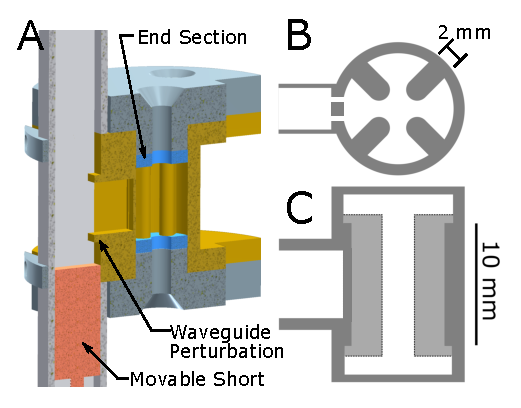
\includegraphics{Kapitel/Ch2-Images/01-TE01UGeometry.eps}
 \caption[Resonator Assembly CAD Drawing.]{A) Half-structure resonator assembly CAD drawing showing the brass resonator (gold), brass end plates (grey), Rexolite end-sections (blue), and copper waveguide (light grey). The waveguide H-type T-junction coupler with inductive obstacles (waveguide perturbation) and brass movable short is also illustrated. The re-entrant geometry is further detailed in B) the top view, showing the re-entrant fins and dual-slot iris, and C) the side view, showing the 10~mm uniform field region-of-interest.}
 \label{Ch2-fig:GEO}
\end{figure}

One solution to increase the stored energy in a UF \cylTE{} is to place a dielectric insert into the cavity. A simulated design of a dielectric UF cavity at X-band frequencies (9.5~GHz) was introduced by Mett \textit{et al.} as a way to increase EPR sensitivity without creating an overly-large cavity. \cite{HydeUFDR2017} The use of dielectric improves the stored energy in the region-of-interest but may exhibit significant frequency dependence with different experimental temperatures. \cite{Hartnett2003} This dependence limits the versatility of a UF cavity. 

In this work, a UF re-entrant cylindrical \cylTE{} cavity at Q-band frequencies (34~GHz) for pulse EPR spectroscopy is introduced, illustrated in Fig.~\ref{Ch2-fig:GEO}. Re-entrant geometries are defined as waveguide structures where perturbations are placed in regions of a large electric field to lower the cut-off frequency of the waveguide and increase the stored energy of the cavity. \cite{ramo1984fields, MITRadWaveguide} In a cylindrical waveguide, for a fixed cut-off frequency, the diameter of the waveguide is decreased as the re-entrant perturbations are extended into the electric field. If one was to make a re-entrant cavity by placing a shorted top/bottom on the waveguide and the resonant frequency is held constant, the stored energy of the cavity would increase as the re-entrant perturbations are increased. When sufficiently close, the re-entrant perturbations behave like plate capacitors. An LGR can be considered a highly re-entrant waveguide operating at cut-off. It is the geometric space between cavities and LGRs that the re-entrant geometry explores. 

In the present design, four 2~mm re-entrant fins are extended into a UF cylindrical \cylTE{} cavity, shown in Fig.~\ref{Ch2-fig:GEO}B, and the UF region-of-interest is elongated to 10~mm ($\lambda_g$ for a TE$_{01}$ mode is 10.2~mm), shown in Fig.~\ref{Ch2-fig:GEO}C. This geometry provides an enhanced efficiency parameter, increased EPR signal intensity, and a uniform H$_1$ field along the sample volume.

In general, UF resonators exhibit several advantages compared to traditional cavities. Typically a cavity geometry has a cosine dependence of H$_1$ in the transverse $z$-direction. With a UF resonator, a region-of-interest is designed to be strictly uniform and can be extended beyond a half wavelength. Uniform field resonators (i) provide better quantitative measurements reducing the need to calibrate the resonator H$_1$ profile \cite{eaton2010quantitative}; (ii) allow the region-of-interest to be extended to provide a larger sample volume, increasing the EPR concentration sensitivity; (iii) can perform reliable continuous-wave (CW) saturation studies \cite{klugsdsl} and more reliable T$_1$ measurements using saturation recovery;  (iv) can be used in pulse experiments with the need for coherent pulses, such as ESEEM/HYSCORE, DEER\cite{pulsejeschke} and ELDOR-detected NMR\cite{COX201763}); and (v) provides uniform excitation for arbitrary-waveform generator (AWG) shaped inversion pulses \cite{stollshaped, shapedpulse} and frequency sweeps. \cite{DOLL201746}

Additionally, an H-type T-junction waveguide coupler with inductive obstacles is used to couple from the transmission waveguide to the resonator, shown in Fig.~\ref{Ch2-fig:GEO}A. The introduction of the inductive obstacles increases the dynamic range of a movable short coupler while reducing the frequency shift during matching. A dual-slot iris is employed to lower the stored energy of the iris and minimize H$_1$ perturbations along the sample volume. \cite{UFLGR2017}

The resonator assembly is fabricated and tested both on the bench and with EPR experiments. Experimental bench test measurements of the resonator characteristics are provided and compared to computer simulations. The H$_1$ profile is measured on the bench using the method of perturbing spheres. 

\section{Methods}
Finite-element simulations were performed on a Fujitsu workstation with dual eight-core Xeon E5-2640 2.60~GHz processors with 15~MB of L2 Cache per chip and 124~GB of system DDR4 RAM. A RAM drive was set up with 16~GB of RAM. The temporary directory and simulation files were stored in the RAM drive to reduce hard-drive bottlenecks. This system has been optimized for simulations with new versions of ANSYS (Canonsburg, PA, USA) High Frequency Structure Simulator (HFSS; v. 18.2) and can take advantage of all sixteen CPUs during finite-element modeling matrix solving. The operating system was Windows~7 64-bit. The eigenmode and driven-mode solvers were used and typical simulation times were 15~minutes. All simulations were performed around 34 GHz.

EPR signal intensity and resonator efficiency values ($\Lambda_{max}$ Eqn.~\ref{ch2-eq:lammax}; $\Lambda_{ave}$ Eqn.~\ref{ch2-eq:lamave}) were calculated using ANSYS HFSS \cite{misrabook} and tabulated for comparison with typical resonator geometries, such as the cylindrical TE$_{011}$ cavity. \cite{generalte011} Two EPR signal conditions are calculated: signal unsaturable (Su; Eqn.~\ref{ch2-eq:su}) and signal saturable (Ss; Eqn.~\ref{ch2-eq:ss}). A 2.8~mm OD and 1.8~mm ID quartz capillary (QSIL GmbH, Ilmenau, Germany) with ice sample ($\epsilon_r=3.17-i0.0035$ \cite{icedielectric} ) was used in the simulations.

After the resonator geometry is designed, it is transferred to the 3D CAD software tool AutoDesk Inventor Professional, where the manufacturing details and geometric dimensions and tolerances are added. The model makers at the Max Planck Institutes for Chemical Energy Conversion and Kohlenforschung (M\"ulheim, Germany) performed the fine-mechanics tooling and die-sink electric discharge machining (EDM) manufacturing needed to fabricate the assembly. The prototype UF re-entrant cylindrical \cylTE{} cavity was fabricated from brass for the resonator body and end-caps. The end-sections were manufactured out of Rexolite plastic.\footnote{Geometric STL files are provided at the Act-EPR website: \textit{http://www.act-epr.org/data.}}

\begin{wrapfigure}{O}{3.5cm}
\centering
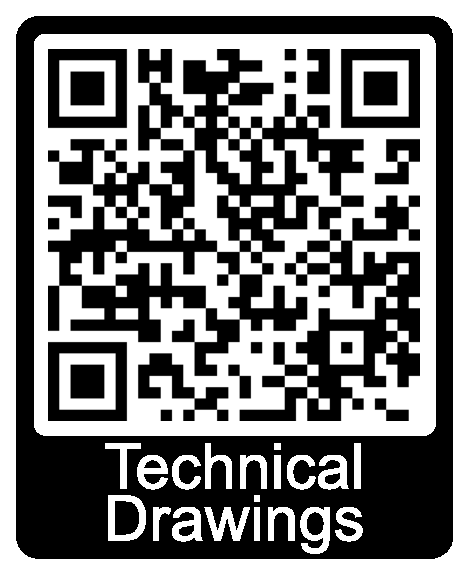
\includegraphics[width=3.5cm]{Kapitel/Appendix/ActEPRdataQR.eps}
\end{wrapfigure}

Resonator characteristics, such as the frequency measurements, $Q_0$-value, over\-/coupling profiles, and sample frequency shifts, were performed on an Agilent 8722ES (now Keysight Technologies; Santa Rosa, CA, USA) vector network analyzer. A 2.8~mm OD and 1.8~mm ID quartz capillary (Vitrocom; Mountain Lakes, NJ, USA) was filled with polystyrene (PS) and a small (0.5~mm diameter) metallic probe was used as the test sample for the method of perturbing spheres. The method of perturbing spheres measures the increase in the microwave frequency as the metallic probe is stepped through the cavity volume. The size of the metallic sphere is chosen so the overall frequency shift was less than 100~MHz.

To further test the B$_{1r}$ field uniformity, a nutation experiment was performed on a Bruker E580 spectrometer with a home-built transceiver accessory operating at Q-band with 10~W of total incident power available. The nutation experiment consists of an initial preparation pulse of varying length ($\tau_n$), fixed delay ($t_1$ of 5000~ns), and a two-pulse detection. The pulse length $\tau_n$ was stepped by 4~ns over 2048 steps and a two-pulse detection echo was recorded. \cite{pulsejeschke} The two-pulse detection echo was configured with a 60~ns and 120~ns pulse with a delay $t_2$ of 300~ns. The scheme is shown in Fig.~\ref{fig:EPRpulse}. The sample consisted of 0.1\% $\alpha$,$\gamma$-Bisdiphenylene-$\beta$-phenylallyl (BDPA) by weight in polystyrene (PS) and was placed in a 2.8~mm OD and 1.8~mm ID  quartz capillary. Two samples were used: The first sample geometry extended the entire length of the cylindrical TE$_{011}$ and re-entrant \cylTE{} cavity length. The second sample geometry was a 9.5~mm sample to place in the 10~mm region-of-interest of the UF re-entrant \cylTE{} cavity.

\section{Uniform Field Design}
\subsection*{General Design Principles.}
Advances in UF resonator design have been recently reviewed. \cite{HydeUFRev2019} In this section, the underlying understanding behind uniform field resonators will be described.

We start by introducing the cylindrical waveguide where the two-dimensional wave equation describes the transverse electric (TE) modes that propagate along the $\pm z$-direction, such that
\begin{equation}
    (\bigtriangledown_t^2 + \beta_{mn}^2) \mathbf{H}_z = 0,
\end{equation}
where $\bigtriangledown_t^2$ is the time-independent Laplacian and $\beta_{mn}^2$ is the wavenumber. The microwave magnetic field $\mathbf{H}_z$ is set by the scalar solution of the transverse components in the $\rho$ and $\phi$ coordinates for a time-varying electromagnetic field $e^{-i \omega t}$. Illustrated in Fig.~\ref{fig:UFwaveguide} is a cylindrical waveguide with a radius of $a$, and the propagation constant can be expressed as a function of the roots of the derivative of the Bessel function of the first kind, such that
\begin{equation}
    \beta_{mn}^2 = \beta_0^2 - \beta_\rho^2 = \beta_0^2 - \bigg(\frac{J_{mn}'}{a}\bigg)^2,
\end{equation}
where $J_{mn}'$ is the $n$-th zero in the first-derivative of the Bessel function $J_m(x)$ and $\beta_0$ is the free-space propagation constant $\omega\sqrt{\epsilon_r \mu_r}$. When $\beta_{mn}$ is set to zero and solved for the frequency the ``cut-off'' condition can be calculated, such that
\begin{equation}
    f_c = \frac{1}{2 \pi \sqrt{\epsilon_r \mu_r}}\frac{J_{mn}'}{a} \qquad [\text{Hz}].
\end{equation}
For the TE$_{01}$ mode, the $J_{01}'$ is approximately 3.832. For simplicity, it is assumed that there is no perturbation from the coupling iris. When the operating frequency $f$ is greater than $f_c$ and the waveguide is infinitely long, the electromagnetic wave will propagate,
\begin{equation}
    \mathbf{H}_z = e^{\pm i\beta_{01}z},\label{propH}
\end{equation}
in the $\pm z$-direction and the wavelength in the waveguide $\lambda_g$ is 
\begin{equation}
    \lambda_g = \frac{2\pi}{\beta_0 \sqrt{1-(f_c/f)^2}} \qquad [\text{m}].\label{wavelength}
\end{equation}
This is illustrated in Fig.~\ref{fig:UFwaveguide}A as the magnitude of the microwave magnetic field (H$_1 = |\mathbf{H}_z|$) plotted along the axis of the geometry. As the operating frequency increases the propagating wavelength approaches the free-space wavelength. \cite{harrington1961time} 

\begin{figure}[ht]
 \centering
 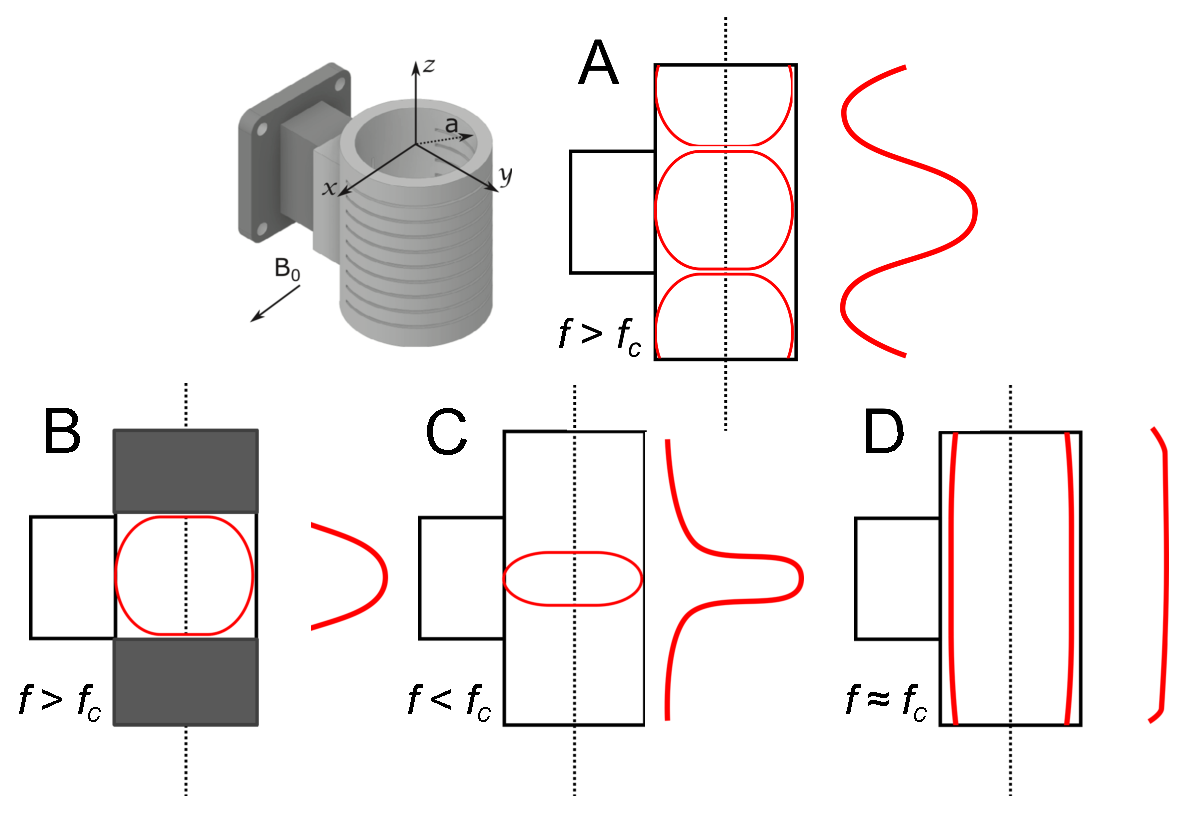
\includegraphics[width=0.9\textwidth]{Kapitel/Ch2-Images/Ch2-UniformFieldWaveguide.eps}
 \caption[Waveguide modes relative to the cut-off frequency]{Waveguide modes relative to the cut-off frequency. A cylindrical waveguide with a radius of $a$ is coupled to a rectangular waveguide, geometry shown. The static magnetic field $B_0$ is indicated in the $x$-direction. A) When the operating frequency $f$ is greater than the cut-off frequency $f_c$ propagation occurs in the $\pm z$-direction. B) When conducting end caps are added, a cavity is created. C) If the operating frequency is less than the cut-off frequency ($f < f_c$) an evanescent mode is formed. D) When the operating frequency approaches the cut-off frequency ($f \approx f_c$) the wavelength becomes infinite, resulting in a uniform field. }
 \label{fig:UFwaveguide}
\end{figure}

By adding end caps to a waveguide a boundary condition is imposed on the TE$_{01}$ propagating mode which forces the tangential electric field to zero. The boundary condition results in a cosine dependence of the H$_1$ within the cavity, illustrated in Fig.~\ref{fig:UFwaveguide}B. With proper dimensions, a TE$_{011}$ cavity is formed. In EPR, a sample is placed in the maximum H$_1$ where the operating frequency (X-band, Q-band, etc) is the frequency of the cavity. 

In the cylindrical waveguide, if the operating frequency $f$ is below the cut-off frequency $f_c$, the propagation constant becomes imaginary. The wave no longer propagates and, instead, $\mathbf{H}_z$ of Eqn.~\ref{propH} becomes evanescent with a reduction that is proportional to the propagation constant. 

Of interest is when the operating frequency approaches the cut-off frequency ($f \approx f_c$). In this case, the wavelength approaches infinity as described by Eqn.~\ref{wavelength}. Under this condition is where uniform field resonators operate. Three characteristics describe the electromagnetic wave in the waveguide at cut-off. First, the wavelength is infinite and, assuming no dampening, the field is strictly uniform in the $\pm z$-direction for an infinitely-long waveguide. Second, the propagation constant is zero indicating no dispersion or phase velocity. This implies that a resonator with a uniform field active-region longer than a wavelength will not have a propagation time and the whole geometry will act as a single-mode cavity.  Finally, a strictly uniform field in the waveguide occurs only when the operating frequency is at the cut-off frequency ($f=f_c$). Any deviation from this equality will result in either a bowed ($f>f_c$) or a concave ($f<f_c$) field profile.

The characteristic impedance of a cylindrical waveguide TE$_{01}$ is defined by 
\begin{equation}
    Z_{01} = \frac{\beta_0 \sqrt{\mu_r/ \epsilon_r}}{\beta_{01}} =\frac{\beta_0 \sqrt{\mu_r/ \epsilon_r}}{\beta_0 \sqrt{1-(f_c/f)^2}} \qquad [\Omega]
\end{equation}
and, therefore, when ($f=f_c$) the impedance approaches infinity. When the waveguide becomes a finite-length, the reflections from the open end-section causes the formation of other modes which degrade the uniform field. If end sections are placed at fixed points along the $z$-axis, a TE$_{01n}$ mode will form at a frequency dictated by the characteristic equation
\begin{equation}
    \omega_{01n} = \frac{1}{\sqrt{\mu_r \epsilon_r}}\sqrt{\bigg(\frac{2 \pi n}{h}\bigg)^2+\bigg(\frac{J_{01}'}{a}\bigg)^2} \qquad [\text{Hz}],
\end{equation}
where $h$ is the height of the resonator and $n$ is the number of half wavelengths that are formed.

To maintain the properties of the uniform field and to satisfy Maxwell's equations for a finite-length waveguide, the end sections must maintain an infinite characteristic impedance. An infinite characteristic impedance is likened to an ``open'' circuit. For a TE$_{01}$ mode, the ``open'' circuit is a perfect-magnetic boundary condition. It is this condition must be matched to the central section. 

Three matching methods were shown to produce this effect: i) over-sized end-sections above cut-off, ii) re-entrant metallic structures that adding capacitance to the end-section, and iii) dielectric end-sections of length $\lambda/4$ placed at each shorted end. All end-section types present an rf open impedance boundary condition to the central cut-off section. These methods are illustrated in Fig.~\ref{fig:UFmethods}.

\begin{figure}[htb]
 \centering
 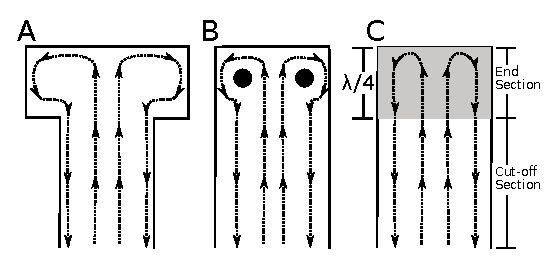
\includegraphics[width=0.7\textwidth]{Kapitel/Ch2-Images/02-UFIllustration.eps}
 \caption[Methods for creating uniform fields in cavities.]{Illustrations of three methods for creating uniform fields in cavities. Region-of-interest at cut-off is matched to A) an  over-sized section, B) a re-entrant end-section with capacitive posts (black circles), C) a dielectric section of length $\lambda/4$ placed at a shorted end. Magnetic fields vectors are illustrated with dotted lines.}
 \label{fig:UFmethods}
\end{figure}

Each method creates an end-section that transfers the characteristic impedance of a ``short'' to an ``open''. One drawback of the uniform field resonator is the frequency dependence of the whole structure. While designing a uniform field resonator, all perturbations must be accounted for, such as the sample, sample holder, end-section dielectrics, iris, and conductivity of the cavity walls. All factors modify the cut-off frequency and are taken into account within the finite-element modeling simulations. Typically uniform field resonators are designed for a range of samples where the non-uniformity is quantified within a dielectric constant range. 

\subsection{Re-Entrant \cylTE{} Cavity Design}
The cylindrical TE$_{011}$ cavity is a standard cavity for Q-band systems. The high Q$_0$-value and sample volume make it a good general-purpose resonator. However, for pulse experiments, the H$_1$ field variation is 50.9\% over the cavity volume. The normalized H$_1$ field for a cylindrical TE$_{011}$ cavity is shown in Fig.~\ref{Ch2-fig:normb1} as a dashed line. In a TE$_{011}$ cavity, when a 90- or 180-degree pulse is applied, a significant portion of the spins in the sample volume is either over or under excited. 

\begin{figure}[htb]\centering
 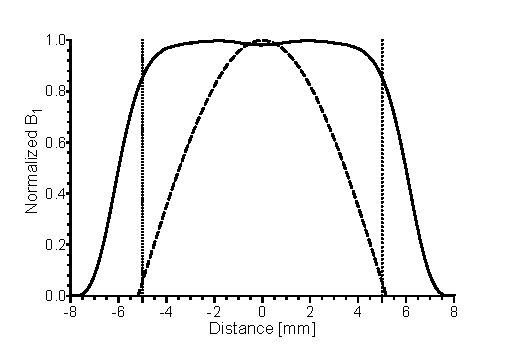
\includegraphics{Kapitel/Ch2-Images/02-TE01UProfile.eps}
 \caption[Ansys HFSS simulation of normalized H$_1$ field.]{Ansys HFSS simulation showing normalized magnetic field H$_1$ down the axis of the cylindrical re-entrant \cylTE{} (solid) compared to the magnetic field down the axis of the cylindrical TE$_{\text{011}}$ cavity (dashed). Dotted lines mark the region-of-interest of the cylindrical re-entrant \cylTE{} cavity. }
 \label{Ch2-fig:normb1}
\end{figure}

If a UF cylindrical \cylTE{} cavity is designed with oversized end-sections (Fig.~\ref{fig:UFmethods}A) and a region-of-interest of 10~mm, as described in Refs.~[3.\kern-0.4em\citenum{mett2001axially}] and [3.\kern-0.4em\citenum{anderson2002}], the H$_1$ variation over the cavity volume is reduced to 20\%. However, the overall $\Lambda_{max}$ is reduced by 39\% compared to a TE$_{011}$ cavity, due to the decrease in stored energy in the entire cavity volume. The decrease in stored energy is caused by the uniform field cavity being geometrically bigger. A solution to increase the resonator efficiency is to introduce re-entrant fins, shown in Fig.~\ref{Ch2-fig:GEO}B, where the electric field is concentrated, shown in \ref{Ch2-fig:EMFields}A, and results in a $\Lambda_{max}$ decrease of 11\% but an overall $\Lambda_{ave}$ increase of 59.6\%. The calculated resonator characteristics of the proposed UF re-entrant \cylTE{} cavity as compared to a TE$_{011}$ and UF cylindrical \cylTE{} cavity with oversized end-sections shown in Fig.~\ref{fig:UFmethods}A are found in Table~\ref{Ch2-table:ansyschar}.

\begin{table}[htb]
\centering
\caption{Ansys HFSS simulated resonator characteristics.}
\label{Ch2-table:ansyschar}
\begin{tabular}{l|c|c|c}
Geometry & \begin{tabular}[c]{@{}l@{}}Cyl. TE$_{\text{011}}$ \\ D/L=1\end{tabular} & \begin{tabular}[c]{@{}l@{}}UF Cyl.\\ \cylTE{}\end{tabular} & \begin{tabular}[c]{@{}l@{}}UF \cylTE{}\\ Re-Entrant\end{tabular} \\ \hline \hline
Frequency & 34.3 & 34.5 & 34.1 \\ \hline
Q$_0$-Value & 13000 & 5900 & 1880 \\ \hline
Signal, S$_u$ & 1 & 0.73 & 1.06 \\ \hline
Signal, S$_s$ & 1 & 0.83 & 1.18 \\ \hline
$\Lambda_{max}$ {[}mT/W$^{1/2}${]} & 1.06 & 0.65 & 0.94 \\ \hline
$\Lambda_{ave}$ {[}mT/W$^{1/2}${]} & 0.52 & 0.52 & 0.83 \\ \hline
$\Delta$H$_1$ & 50.9\% & 20\% & 11.7\%
\end{tabular}
\end{table}

\begin{figure}[htb]\centering
 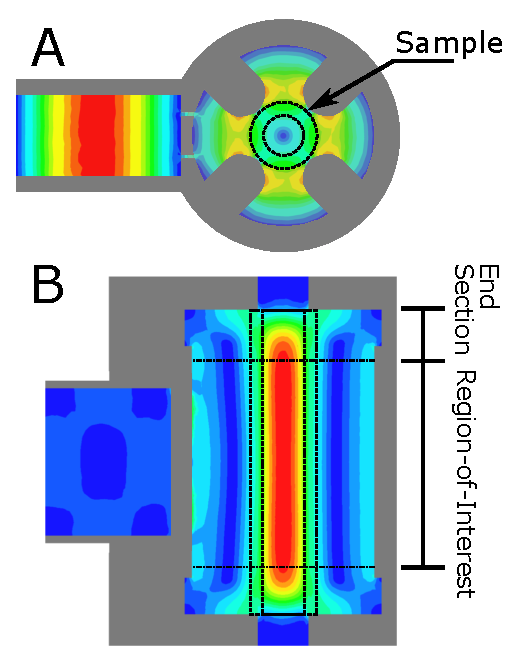
\includegraphics{Kapitel/Ch2-Images/03-TE01UEMFields.eps}
 \caption[Simulation of the microwave fields.]{Ansys HFSS simulation showing the magnitude of the microwave A) electric and B) magnetic fields of the uniform field re-entrant cylindrical \cylTE{} cavity. Each iris is 0.2~mm wide and extends over the entire waveguide length.}
 \label{Ch2-fig:EMFields}
\end{figure}

Using Ansys HFSS, a UF re-entrant \cylTE{} cavity is designed by the following procedure: (i) An eigenmode solution of the central section with a sample is simulated with a perfect magnetic field boundary condition. This provides the resonant frequency of the central section at cut-off with a sample. (ii) The region-of-interest is extended to 10~mm and Rexolite end sections are added to the simulation at a nominal height. (iii) The end sections are varied until the eigenfrequency matches the cut-off frequency. (iv) An iris is introduced and the end sections are adjusted to accommodate the frequency shift. (v) Once completed, the resonator is imported into AutoDesk Inventor and prepared for fabrication. 

By properly matching the end sections, a uniform H$_1$ field can be realized, illustrated in Figs.~\ref{Ch2-fig:EMFields}B. The normalized H$_1$ field profile is shown in Fig.~\ref{Ch2-fig:normb1} as a solid line. In the 10~mm region-of-interest, the H$_1$ field profile is 98\% uniform. 

\begin{figure}[htb]\centering
 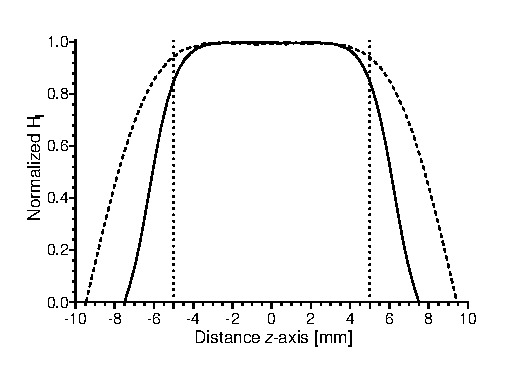
\includegraphics{Kapitel/Ch2-Images/ComparisonOfEndSections.eps}
 \caption[Ansys HFSS simulation comparing oversized and re-entrant end sections.]{Ansys HFSS simulation showing normalized H$_1$ field of the cylindrical re-entrant \cylTE{} (solid) compared to a \cylTE{} cavity with oversized end-sections depicted in Fig.~\ref{fig:UFmethods}A (dashed). Dotted lines mark the region-of-interest of the cylindrical re-entrant \cylTE{} cavity. }
 \label{Ch2-fig:normb1compare}
\end{figure}

As shown in Fig.~\ref{Ch2-fig:GEO}C, the re-entrant fins do not extend fully into the end section region. This design choice causes the end section to be electrically larger (shorter wavelength, $\lambda_g$) and reduces the end-section size needed to produce the matching criteria for the region-of-interest. As shown in Fig.~\ref{Ch2-fig:normb1compare}, the roll-off in the current design is steeper compared to a \cylTE{} cavity with oversized end-sections designed from Fig.~\ref{fig:UFmethods}A. Decreasing the roll-off region of the resonator minimizes the sample volume that is excited by non-uniform fields.

\subsection{Dual-Slot Iris Design}

A dual-slot iris was designed to couple the UF re-entrant \cylTE{} cavity. The use of dual-slot iris reduces H$_1$ perturbations due to the stored energy in the iris. For UF resonators, the dual iris also reduces coupling to higher-order modes that may exist because of the large length of the region-of-interest. \cite{UFLGR2017} The size of a single capacitive iris needed to couple the resonator was 0.45~mm. A dual-slot iris, each iris was 0.2~mm thick, was used to achieve the same coupling. The geometry is shown in Fig.~\ref{Ch2-fig:GEO}A and \ref{Ch2-fig:GEO}C and the electric field profile in Fig.~\ref{Ch2-fig:EMFields}A.

\section{Results}
The Q$_0$-value of the UF cavity was measured to be 1330 with a distilled water ice sample at a frequency of 33.95~GHz. Additionally, the frequency shift of the re-entrant \cylTE{} cavity as the match was adjusted from critically coupled (-45~dB ) to over-coupled (-9~dB) was 6.96~MHz, consistent with simulations of Fig.~\ref{Ch2-fig:waveguide}C. 

\begin{figure}[htb]\centering
 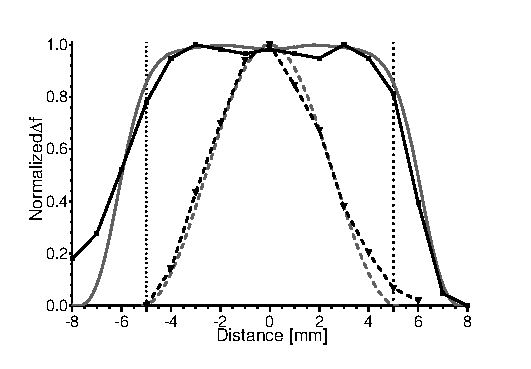
\includegraphics{Kapitel/Ch2-Images/05-TE01Uperturb.eps}
 \caption[Measured magnetic field using perturbing spheres.]{Method of perturbing spheres showing the normalized $\Delta$f along the axis of the cylindrical re-entrant \cylTE{} (solid) compared to the cylindrical TE$_{\text{011}}$ cavity. Dotted lines mark the region-of-interest of the cylindrical re-entrant \cylTE{} cavity.  Comparison to Ansys HFSS simulations are shown in grey.}
 \label{Ch2-fig:perturb}
\end{figure}

The change in frequency due to the presence of a small metallic probe is shown in Fig.~\ref{Ch2-fig:perturb}. Measurements of the UF re-entrant \cylTE{} cavity are shown as a solid line and match well with simulations. For comparison, measurements of the cylindrical TE$_{011}$ is presented as a dashed line. The profiles here should be compared to the Ansys HFSS simulations of Fig.~\ref{Ch2-fig:normb1}, shown as gray for convenience. 


\subsection{Waveguide H-type T-junction Coupler with Inductive Obstacles}
\begin{figure*}[htb]\centering
 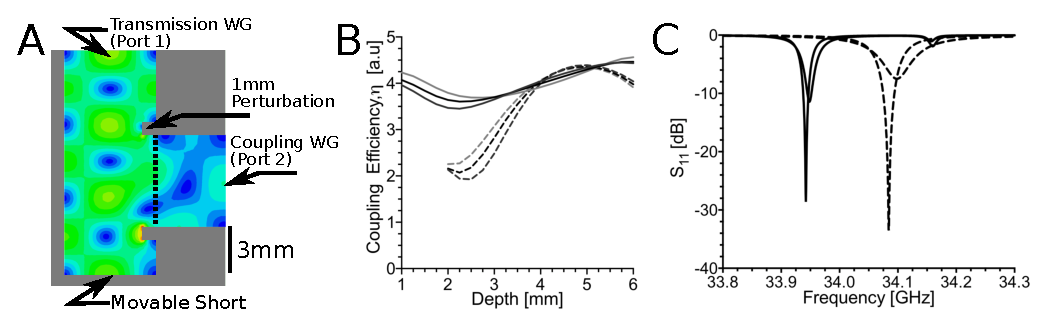
\includegraphics[width=\textwidth]{Kapitel/Ch2-Images/04-CouplingPert.eps}
 \caption[Waveguide H-type T-junction coupler geometry.]{A) Waveguide H-type T-junction coupler geometry with perturbations showing the transmission waveguide, coupling waveguide, and movable short. B) Ansys HFSS simulations showing the coupling efficiency without (solid) and with 1~mm perturbations (dashed) for three frequencies (33.5, 34, and 34.5~GHz, red, black, blue, respectively). C) Simulations showing the reflection coefficient S$_{\text{11}}$ without (solid) and with 1~mm perturbations (dashed) at depths of 3.5~mm and 5~mm of the movable short (coupled and over-coupled; black and red). Operating frequency is 34.09~GHz.}
 \label{Ch2-fig:waveguide}
\end{figure*}

For the resonator assembly to fit in a 40~mm diameter cryostat, an H-type T-junction coupler was implemented with a sliding short matching system. This sliding short is typical for a Q-band TE$_{011}$ cavity and provides a robust coupling method for room temperature to sub-10~K measurements. \cite{generalte011} Typically coupling to a TE$_{011}$ cavity is performed by introducing an iris to the H-plane sidewall of the transmission waveguide. However, due to the oversized end-sections, a coupling waveguide of 5.07~mm length is introduced perpendicular to the transmission waveguide, illustrated in Fig.~\ref{Ch2-fig:waveguide}A. 

Three features describe an H-Type T-junction coupler: (i) The H-type T-junction coupler is similar to the H-arm of a magic-Tee coupler. \cite{ramo1984fields, MITRadWaveguide} (ii) The coupling waveguide is at least $\lambda_g$/2 in length. (iii) To maximize coupling, an ``inductive obstacle'' on the sub-wavelength H-type T-junction is introduced to the transmission waveguide. The ``inductive obstacle'', described by Ref~[3.\kern-0.4em\citenum{MITRadWaveguide}] as a ``Window Formed by One Obstacle'', is introduced to the H-plane around the coupling waveguide and extends 1~mm into the transmission waveguide, illustrated in Fig.~\ref{Ch2-fig:waveguide}A. This inductive obstacle creates a favorable geometry for electric field coupling and increases coupling efficiency. 

Plotted in Fig.~\ref{Ch2-fig:waveguide}B is the simulated coupling efficiency transmission can be calculated using an overlap integral \cite{born} of the two electric fields and is defined as
\begin{equation}
    \eta = \frac{\left| \int E_{t} \cdot E^*_{c} dA\right|^2}{\int \left|E_t\right|^2 dA \int \left|E_c\right|^2 dA},
\end{equation}
where $E_{t} \cdot E^*_{c}$ represents the electric field coupling over the waveguide interface area between the electric field of the transmission waveguide ($E_{t}$) and the coupling waveguide ($E_{c}$) at the interface area A, shown as a dotted line in Fig.~\ref{Ch2-fig:waveguide}A. 

The coupling efficiency between port 1 at the transmission waveguide and port 2 at the coupling waveguide is shown in Fig.~\ref{Ch2-fig:waveguide}B, where the coupling efficiency without the waveguide perturbations (solid) and with 1~mm perturbations (dashed) is plotted. Three frequencies (33.5, 34, and 34.5~GHz, light grey, black, dark grey, respectively) are used to show the frequency dependence. Lower coupling efficiency under-couples the resonator. The resonator is critically coupled when the movable short is around 3.5~mm depth at 34~GHz and maximum over-coupling occurs at 5~mm. The waveguide H-type T-junction coupler with the perturbation illustrates a more dynamic range in coupling for the same distance and a flatter response for maximum over-coupling with a 1~GHz frequency range. To produce the same coupling range without the waveguide perturbations the iris must be 25\% larger. A larger iris leads to inhomogeneity of the H$_1$ field around the iris and in the region-of-interest. 

The UF re-entrant \cylTE{} cavity is designed to be over-coupled. Shown in Fig.~\ref{Ch2-fig:waveguide}C is the effect of the movable short on the reflection coefficient S$_{\text{11}}$ of the UF re-entrant \cylTE{} with a range of coupling positions (3.5 and 5~mm, coupled and over-coupled). The resonator microwave frequency shift with coupling is reduced form 14.4~MHz to 8.2~MHz using the H-type T-junction coupler with perturbations. Lower microwave frequency pulling occurs due to a reduction in the stored energy in the region of the coupler. 

Additionally, for the same resonator geometry, there is a 145~MHz shift in operating frequency from its eigenfrequency of 34.1~GHz due to the impedance of the coupler without the perturbations. The coupler without perturbations has more stored energy and more reactance, consistent with the understanding of coupling systems with frequency dependence. \cite{Mett2009} This causes a shift in the real part of the microwave frequency to compensate for the imaginary part of the assembly reactance and makes the assembly more frequency-dependent. 

\subsection{Experimental Results}
Shown in Fig.~\ref{Ch2-fig:nutation} are the data from the nutation experiment. Dotted lines represent the center of the nutations, while dashed lines show 50\% signal markers. The cylindrical TE$_{011}$ cavity data was taken with the BDPA sample extending the entire cavity length and plotted in Fig.~\ref{Ch2-fig:nutation}A. For a 120~ns $\pi$-pulse the power was set to 2.5~W. In Fig.~\ref{Ch2-fig:nutation}B, the UF re-entrant \cylTE{} cavity with the BDPA sample extending the entire cavity length is shown. For a 120~ns $\pi$-pulse the power was set to 5~W. A second sample with 9.5~mm length was centered in the UF re-entrant \cylTE{} cavity region-of-interest. Experimental nutation data are plotted in Fig.~\ref{Ch2-fig:nutation}C and for a 120~ns $\pi$-pulse the power was set to 5~W.

\begin{figure}[htb]\centering
 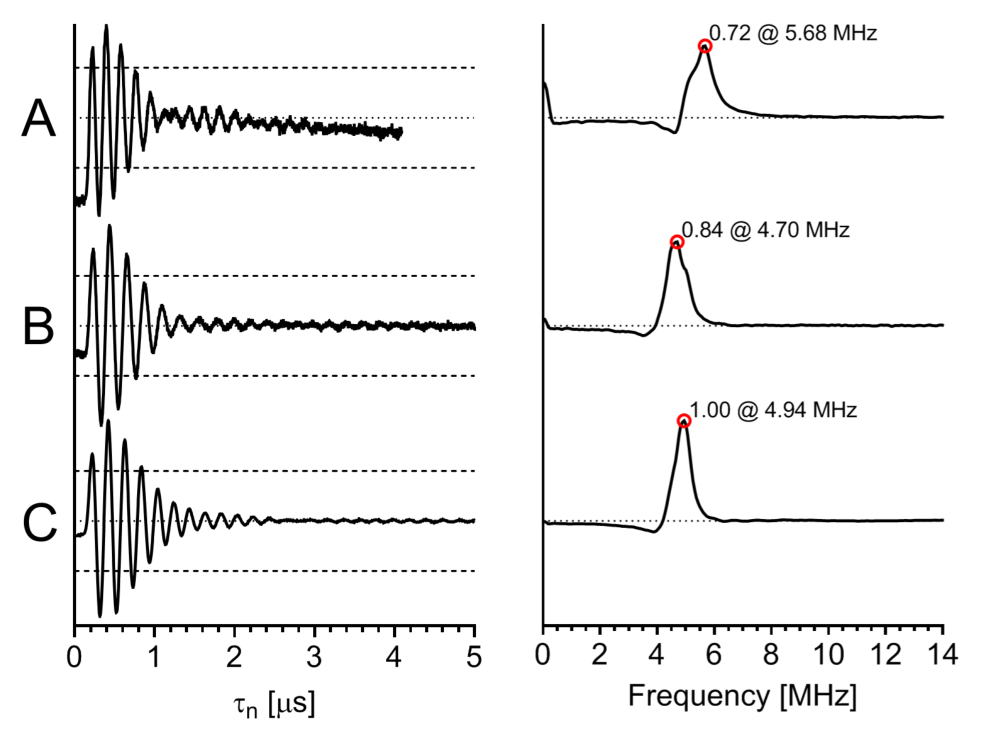
\includegraphics[width=0.8\textwidth]{Kapitel/Ch2-Images/06a-Nutation.eps}
 \caption[Nutation experiment comparison.]{Nutation experiment on a BDPA sample performed using the A) cylindrical TE$_{011}$ cavity, B) the uniform field re-entrant \cylTE{} cavity with the sample extending the entire length and C) a 9.5~mm sample centered in the region-of-interest. Pulse lengths were 120~ns for $\pi$-pulse and the preparation pulse length was stepped 4~ns. Dotted lines show the nutation center, while dashed lines show 50\% signal markers. The real part of the Fourier transform of the nutation experiment is shown on the left with the peak amplitude and corresponding frequency marked.}
 \label{Ch2-fig:nutation}
\end{figure}

Nutation experiments show good results in terms of increased sensitivity and uniformity of the H$_1$ field. The nutations using the UF re-entrant \cylTE{} cavity with the sample extending the entire length show clear improvements over the data from the cylindrical TE$_{011}$ cavity, shown in Fig.~\ref{Ch2-fig:nutation}A and \ref{Ch2-fig:nutation}B, respectively. 

The UF re-entrant \cylTE{} cavity with the 9.5~mm sample only in the region-of-interest, shown in Fig.~\ref{Ch2-fig:nutation}C, has the nutations further extended and the initial off-set is further minimized. These data show the advantages of uniform field cavities. Three differences of note are: (i) The signal-to-noise ratio is improved by at least 40\% and the initial offset is reduced by 50\%. (ii) The first-order linear background subtraction is not adequate for the cylindrical TE$_{011}$ cavity. A higher-order background exists that cannot be easily corrected. (iii) A nutation signal phase-inversion is exhibited in  Fig.~\ref{Ch2-fig:nutation}A at 1200~ns and another at 2400~ns, while only one inversion at 2800~ns is noticeable in Fig.~\ref{Ch2-fig:nutation}B. This oscillatory phase-inversion has been experimentally determined to be due to inhomogeneity of $\mathbf{B}_{1r}$, seemingly at the top and bottom of the resonator. The nutation signal phase-inversion is shown to be minimized in Fig.~\ref{Ch2-fig:nutation}C, but can be deliberately increased by moving the sample outside of the region-of-interest.

Also shown in Fig.~\ref{Ch2-fig:nutation} is the real part of the Fourier transform of the data. In this display, the broadening of the peak is determined by the inhomogeneity of $\mathbf{B}_{1r}$. \cite{pulsejeschke} It is clear that the UF re-entrant \cylTE{} cavity with the sample centered in the region-of-interest (Fig.~\ref{Ch2-fig:nutation}C) has the sharpest feature. The intensity at 0~MHz shown prominently in Fig.~\ref{Ch2-fig:nutation}A and reduced in Fig.~\ref{Ch2-fig:nutation}B is directly caused by the inhomogeneity of the magnetic field. The majority of this component is removed in Fig.~\ref{Ch2-fig:nutation}C. 

\section{Discussion}

Dielectric loading variations due to different samples change the cut-off frequency of the region-of-interest, and thus, the uniformity condition of the resonator. Shown in Fig.~\ref{Ch2-fig:dielectric} is the simulated microwave magnetic field squared (H$^2_1$) profile of the UF re-entrant cylindrical \cylTE{} cavity for a range of dielectric constants ($\epsilon_r$ ranges from 1 to 5 in integer steps, with a loss tangent of 0.005) for a fixed Rexolite end section geometry. The microwave magnetic field squared is used to highlight the differences and is proportional to the EPR signal. The frequency is shifted due to the change in the real part of the dielectric from 1 to 5. The frequencies  34.492, 34.206, 33.910, 33.592, 33.264~GHz, $\epsilon_r$ from 1 to 5 respectively, which affects the cut-off and homogeneity of H$_1$. 

\begin{figure}[htb]\centering
 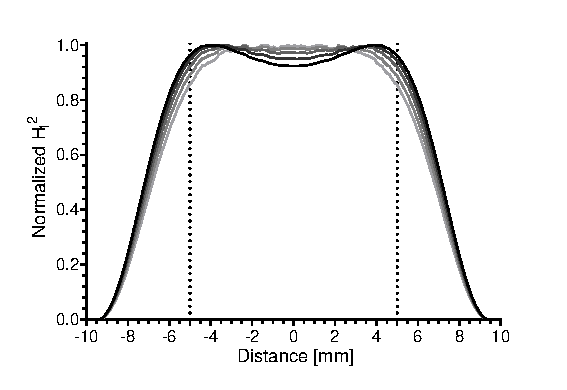
\includegraphics{Kapitel/Ch2-Images/07-TE01UdielectircA.eps}
 \caption[Ansys HFSS simulations of with varying samples.]{Ansys HFSS simulations of the microwave magnetic field squared (H$^2_1$) along the axis of the UF re-entrant cylindrical \cylTE{} cavity for a range of dielectrics. The dielectric constant, $\epsilon$, is varied from 1 to 5 (dark to light) with a fixed end section geometry. Dotted lines mark the region-of-interest of the cylindrical re-entrant \cylTE{} cavity.  The microwave magnetic field squared is used to highlight the differences and is proportional to the EPR signal. }
 \label{Ch2-fig:dielectric}
\end{figure}

The $\Lambda_{ave}$ of the UF re-entrant \cylTE{} resonator is lower than expected by about 40\%. This is mostly due to the Q$_0$-value being lower than expected. The lowering of the Q$_0$-value is due to the construction of the prototype resonator out of brass and higher losses in the Rexolite plastic than anticipated. Changing the resonator body to solid silver and experimenting with different plastics would be advantageous. 

Higher stored energy in the coupling and iris region makes the system more frequency-dependent. The frequency dependence of the H-type T-junction coupler without inductive perturbations was shown to have a large effect on the coupling efficiency, shown in Fig.~\ref{Ch2-fig:waveguide}. Additionally, by extending the iris over the entire length of the waveguide H-plane, a long-slot iris is created. \cite{Mett2009} The long-slot iris exhibits lower stored energy than a resonant iris or inductive hole and minimizes H$_1$ field perturbations. By splitting the long-slot iris to a dual-slot iris, the stored energy and frequency dependence is further reduced. In general, the reduction of stored energy outside of the resonator reduces the frequency dependence when tuning, matching, or changing samples. These design criteria are critical for UF resonators. 

\begin{figure}[htb]\centering
 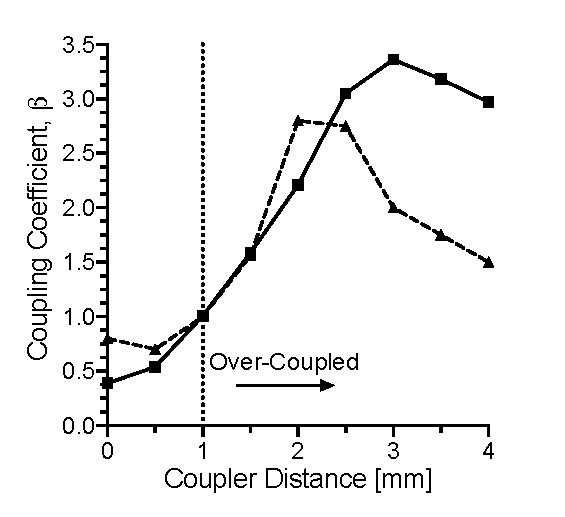
\includegraphics{Kapitel/Ch2-Images/08-couplingcoeff.eps}
 \caption[Bench measurements of the coupling coefficient.]{Bench measurements on the vector network analyzer of the coupling coefficient $\beta$  for the re-entrant \cylTE{} cavity with H-type T-junction coupler and long slot iris (solid) compared to the cylindrical TE$_{011}$ cavity with slot iris from Ref.~[3.\kern-0.4em\citenum{generalte011}] (dashed).}
 \label{Ch2-fig:coupling}
\end{figure}

Shown in Fig.~\ref{Ch2-fig:coupling} are vector network analyzer measurements of the coupling coefficient $\beta_c$ for the re-entrant \cylTE{} cavity with H-type T-junction coupler and long slot iris (solid) compared to the cylindrical TE$_{011}$ cavity with slot iris from Ref.~[3.\kern-0.4em\citenum{generalte011}]. The measured data shows better over-coupling performance for the re-entrant \cylTE{} cavity which corresponds to a larger bandwidth by the equation
\begin{equation}
    Q_L = \frac{Q_0}{\beta_c+1}, \label{q0eqn}
\end{equation}
where the loaded Q-value, Q$_L$, is proportional to bandwidth by $1/\Delta f$. \cite{ramo1984fields} With a lower initial Q$_0$ value, the re-entrant \cylTE{} cavity has a significant increase in bandwidth for comparable EPR signal. The re-entrant \cylTE{} cavity has a calculated bandwidth of approximately 110~MHz, while the cylindrical TE$_{011}$ cavity of Ref.~[3.\kern-0.4em\citenum{generalte011} has a calculated bandwidth of 46~MHz (Q$_0$ of 2400).

Finally, in the $x$- and $y$-direction the H$_1$ field exhibits some variation. A smaller inner diameter capillary (with the same outer diameter) could be used to improve this variation but will sacrifice EPR signal intensity. However, the $x$- and $y$-direction variation is already 15\% better in a re-entrant geometry compared to the cylindrical TE$_{011}$ cavity from both a ``sucking-in'' effect of the quartz capillary and more confined electric field profile, as shown in Fig.~\ref{Ch2-fig:EMFields}. The capillary geometry of 2.8~mm OD and 1.8~mm ID was chosen to be compatible with our current standard Q-band capillary tubes. 

\section{Conclusions}
A uniform field re-entrant cylindrical \cylTE{} cavity has been designed, fabricated, and tested to improve pulse EPR experiments. The microwave magnetic field, H$_1$, has been calculated and confirmed by measurements to be 88.3\% uniform over the entire cavity and 98\% uniform over the region-of-interest. By introducing re-entrant fins to a UF cylindrical \cylTE{} cavity, the Q-value of the re-entrant \cylTE{} cavity is lowered, but the resonator efficiency and the stored energy is increased. This new geometry yields similar signals as the standard cylindrical TE$_{011}$ while increasing $\Lambda_{ave}$ by approximately 60\%. The increase of $\Lambda_{ave}$ affects pulse EPR experiments in two ways: (i) less microwave power is needed for the same tip angle; and (ii) the majority of the sample is excited at the same tip angle. 

Initial results using a brass prototype resonator have shown significantly improved data quantified by the nutation experiments. In this work, it has been shown that a UF re-entrant geometry can provide an enhanced efficiency parameter, increase EPR signal intensity, larger bandwidth and a uniform H$_1$ along the sample volume to improve pulse EPR experiments. Future work includes a gold-plated second-generation resonator, ESEEM, HYSCORE and ELDOR-detected NMR experiments (EDNMR), and extending the UF re-entrant \cylTE{} cavity to W-band frequencies.

Uniform field resonators have several advantages for both continuous-wave and pulse EPR experiments. In continuous-wave EPR at low power, a uniform field resonator with the same active sample volume as a traditional cavity will increase the EPR signal by the ratio of the square of the H$_1$ between the cavities. However, in a traditional cavity at an incident power high enough to cause saturation, a distribution of H$_1$ exists incident on the sample. By increasing the uniformity of H$_1$ all spins along the sample length are saturated at the same value. This has direct implications for the quality of data obtained from a sampled under saturation conditions. For example, saturation transfer experiments where the out-of-phase component of the phase-sensitive detector is used as an indicator of molecular motion as the sample is driven under saturation conditions. \cite{SaturationTransfer2005} 

Uniform field resonators used in pulse experiments will not only increase the EPR signal, but time-dependent effects that may lead to complex backgrounds can be reduced. The effects of non-uniform magnetic flux density excitation are relatively unknown as the number of pulses increase in more sophisticated sequences. In general, uniform field resonators increase the quality of pulse data and reduce artifacts. 


{\renewcommand{\bibsection}{\clearpage\section*{\bibname}\markboth{\bibname}{\bibname}}
\renewcommand{\bibname}{CHAPTER 3. REFERENCES}
\bibliographystyle{elsarticle-num}
\bibliography{Kapitel/Ch3-References}   % name your BibTeX data base
}
\chapter[Weak Coupling of Meta-Materials for FD-FT THz EPR]{Weak Coupling of Meta-Materials with Ensemble of Electron Spins: Surface EPR Signal Enhancement in the THz Bandgap.}
\chaptermark{FD-FT THz EPR with Meta-Materials}
\setcitestyle{citesep={,\,\thechapter.}}

As the microwave frequency is increased, single-mode cavity resonators and samples become geometrically small. At even higher frequencies (> 263~GHz), the further reduced dimensions prevent the fabrication of conventional resonators due to technical limitations. To increase sensitivity at higher frequencies the use of non-resonant structures, such as the so-called ``bucket'' sample holder, can be employed. In these non-resonant structures, the sample volume is increased to fill the bucket providing a large filling factor $\eta$ with a Q$_0$-value effectively at unity. \cite{grinbergVHF} However, the shape of the bucket resonator is adapted to powders or solutions filled in tubes, and is not optimal for studies of thin films or surfaces. The ability to measure thin films is crucial for the study of a variety of interesting samples, such as thin magnetic films, thin-film electronic devices, solar cells or other 2D paramagnetic samples.

The transition from volume samples, such as those in single-mode cavity resonators, to planar samples, requires a concentration of the magnetic component of the time-varying excitation field on a cross-sectional area. For example, the plane-concave Fabry-P\'{e}rot resonator, which comprises of a resonant structure with one concave mirror and one flat mirror, forms a standing-wave pattern with a maximum magnetic field on the flat-mirror surface. \cite{grinbergVHF} Plane-concave Fabry-P\'{e}rot resonators exhibit very high Q-values and, due to the simplified geometry, can be designed to operate at frequencies higher than 200~GHz. \cite{Clarke1982Fabry, BraakmanFabry} However, the resonator geometry still scales with frequency and, due to standing-waves within the resonator, the filling factor can be quite low for thin films. To maximize the EPR signal intensity for thin-film samples, a resonant geometry where the cross-sectional sample area is not dependent on the operating frequency and the filling factor is maximized is required. 

One solution is to create a series of single nano-resonators that can be placed in periodic sequences to form a large two-dimensional array. Despite the periodic nanostructure, the incident excitation wave interacts with the surface as a bulk material. \cite{Yen04} This bulk material, called a meta-material, can be characterized by the single and periodic geometry, mutual coupling between elements, eigenfrequency, and $Q_0$-value. Meta-material characteristics can then be used to determine the frequency-dependent properties of the bulk material. The frequency-dependent properties of meta-materials were theoretically proposed in 1968 as materials with bulk properties that mimic frequency-dependent negative electric-permittivity $\epsilon_r(\omega)$ and magnetic permeability $\mu_r(\omega)$. \cite{Veselago68} The ability to tune these properties allows a negative refraction index to be designed for perfect lensing, i.e. images with better resolution than the diffraction limit. \cite{Smith04} Unlike single-mode cavities that require the sample to be placed on an axis of maximum sensitivity, meta-materials can provide a bulk material-like enhancement of a sample at a surface.

Recently, it was found that the split-ring resonator (SRR) geometry at sub-wavelength dimensions can be placed periodically on a surface and behave as a meta-material over a broad frequency range. \cite{Smith00,Yen04,Linden04} This first realization was shown for the low GHz range, \cite{Smith00} then for around 1~THz, \cite{Yen04} and for 100~THz. \cite{Linden04} The negative $\mu_r(\omega)$ leads to a resonance effect in the non-magnetic meta-material. Interestingly, meta-material surfaces operating in the THz region have been employed for ultra-sensitive bio-sensing due to their ability to sense small dielectric changes on a surface. \cite{C7NR03824K} For a bio-sensing experiment, THz frequency microwave fields are incident on the meta-material and the resulting transmission is monitored for changes as bio-material passes the resonant geometry. \cite{Lee2017}

\begin{figure}[htpb]
\centering
  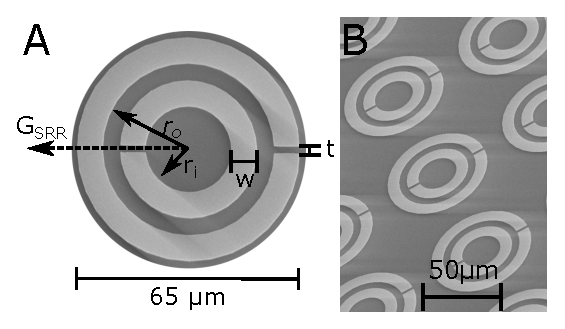
\includegraphics{Kapitel/Ch3-Images/01-Measurements.eps}%
  \caption[Microscope image of the SRR geometry.]{ A) Microscope image of the fabricated profile of the dual-ring split-ring resonator (SRR) on quartz glass. In this work dimensions are as follows: r$_o$ is 25~$\mu$m, r$_i$ is 12.5~$\mu$m, w is 7.5~$\mu$m, and t is 2~$\mu$m. The vector parallel to the gap is illustrated as G$_{SRR}$. B) To create a meta-metallic surface each SRR element is spaced 80~$\mu$m apart from center-to-center.}
  \label{ch3-fig:sizes}
\end{figure}

Herein, the characterization and experimental realization of a meta-material by a split-ring resonator array (SRRs) for the use of detecting EPR transitions in the 100~GHz to 1~THz frequency range (3.34-33.36~cm$^{-1}$; THz-bandgap) is presented. The SRRs have an operating frequency of approximately 420~GHz (14~cm$^{-1}$; free-space wavelength $\lambda$ of 713.8~$\mu$m). A single SRR outer diameter is 65~$\mu$m, geometry shown in Fig.~\ref{ch3-fig:sizes}A. Therefore each SRR is less than 1/10th of a wavelength and is spaced 80~$\mu$m from the next resonator in a periodic fashion creating the bulk-material. The SRRs, shown in Fig.~\ref{ch3-fig:sizes}B, were placed on a quartz substrate that has an overall diameter of 12~mm providing very large surface area for an operating frequency of 420~GHz.

The results were duplicated with a lumped-circuit transmission\-/line analytic model. The lumped-circuit transmission\-/line model, unlike current literature, takes into account both inductive and capacitive coupling. This distinction is important when the interaction of magnetic resonance coincides with the resonant frequency of the SRRs.

The validity of the analytical model was established and used to further understand the interactions that arise between the meta-material and the electron-spins ensemble. Furthermore, the analytical model was used to define the system in terms of weak- and strong-coupling. Through this new understanding, the potential of meta-material arrays for resonant EPR detection at very high frequencies for thin-film samples is illustrated. 

\section{Methods}
To characterize the SRRs Frequency-Domain Fourier-Transform THz-EPR (FD-FT THz EPR) experiments were employed. FD-FT EPR is a method to detect magnetic transitions in the THz-bandgap using an interferometer and bolometer detector. \cite{Schnegg09,NEHRKORN201710} Such methods allow for broad-band detection of EPR in the frequency domain while stepping the static magnetic field through the EPR resonance condition. Over the last decade, several other EPR instruments were built which operate at microwave frequencies in the THz-bandgap. \cite{Disselhorst95, Hassan00, vanTol05, Zvyagin09, Takahashi09, C7CP07443C, Lu2017} The SRRs were characterized and coupled to the electron-spin ensemble of a thin film of the high-spin Fe-ion cluster hemin. The high-spin Fe EPR signal was collected by following the feature located at the effective $g=6$ position which passes through the frequency of the split-ring resonator as the magnetic field is increased. 

Coherent broadband excitation profiles are required for FD-FT EPR experiments. However, at such frequencies, excitation power is limited (milliwatt range) and the frequency range of such sources is limited making frequency domain experiments rather impractical. To overcome these limitations, an alternative excitation and detection scheme has been developed for FD-FT EPR to be performed using a high-power broadband source, such as a coherent beam-line from the BESSY II synchrotron (Helmholtz-Zentrum Berlin; Berlin, DE). From this setup, the EPR spectrum can be ascertained with good signal-to-noise ratio making FD-FT EPR a powerful technique to obtain accurate zero-field splitting parameters. \cite{Nehrkorn13,Nehrkorn15,NEHRKORN201710}

\begin{figure}[htpb]
\centering
  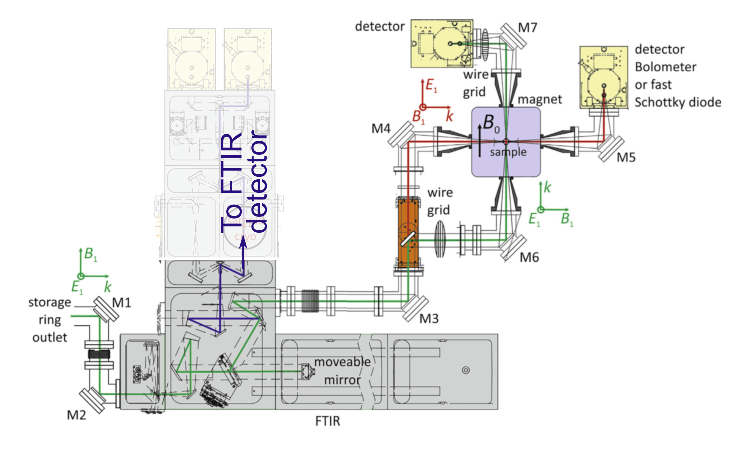
\includegraphics{Kapitel/Ch4-Images/Ch4-ExperimentSetup.eps}%
  \caption[Schematic Overview of FT-FD THz-EPR setup.]{Shown is the schematic overview of the FT-FD THz-EPR setup. The incident wave from the storage ring is sent through a series of mirrors (M1-M3) as it is guided through an FTIR interferometer setup (green line). Here, the polarization of the wave can be rotated (M4) and sent through the static magnetic field (\textbf{B}$_0$) to M5 and a bolometer detector (red line) or reflected directly (M6) through the static magnetic field (\textbf{B}$_0$) to M7 and a bolometer detector (green line). The sample is placed in the static magnetic field. An alternative path allows FTIR to be performed (blue line).}
  \label{ch4-fig:ExFDFTSetup}
\end{figure}

Frequency-Domain Fourier-Transform THz-EPR experiments in this work were performed at the synchrotron BESSY II. The experimental setup is shown in Fig.~\ref{ch4-fig:ExFDFTSetup} \cite{Schnegg09,Nehrkorn13} In short, intense and coherent broadband linearly-polarized radiation in the THz-gap is provided by the synchrotron BESSY II from the storage ring. \cite{AboBakr02} After passing through the interferometer of an FTIR spectrometer (movable mirror), linearly-polarized THz radiation passes a rooftop mirror which allows rotation of the THz TEM-wave polarization to any direction perpendicular to the direction of propagation $\vect{k}$, depicted as the green or red path. Next, the THz radiation is guided through a superconducting magnet (Oxford Spectromag, $\pm$11~T maximal field). The sample is inserted in a variable temperature Dewar (2-300~K) inside the magnet. Finally, the THz radiation is detected with a highly sensitive Si bolometer immersed in a pumped liquid-Helium bath (1.3~K). In this work, the experimental resolution was set to 0.2~cm$^{-1}$ (max resolution: 0.0063~cm$^{-1}$). For each magnetic field step, a full broadband energy spectrum is collected. 

The final set of FD-FT THz EPR spectra were obtained by field division of two subsequent spectra measured at a temperature of 2~K and spaced 0.2~T apart. The field division of spectra was found to produce a more reliable spectrum when comparing features with simulations. \cite{Schnegg09,Nehrkorn13,NEHRKORN201710} The field division process is illustrated in Fig.~\ref{ch4-fig:FDS}. First, a spectrum is measured at B$_0$ indicated on the y-axis of Fig.~\ref{ch4-fig:FDS}, for example, 5.2~T. The collected spectrum was divided by a spectrum measured at B$_0 - 0.2$~T, for example, 5~T. In this example, the result is shown in red in Fig.~\ref{ch4-fig:FDS}. This is equivalent to a field-stepped modulation and only field-induced changes are visible. A positive deviation indicates that the absorption was stronger at B$_0 - 0.2$~T than at B$_0$. In the opposite case, the spectra deviate negatively. This effectively results in a ``first derivative-like'' spectrum.

\begin{figure}[htp]
\centering
  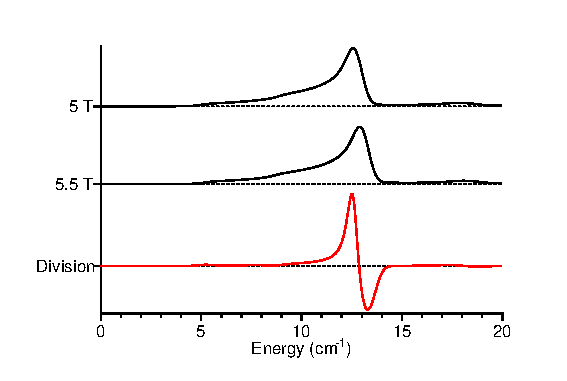
\includegraphics[width=0.8\textwidth]{Kapitel/Ch4-Images/Ch4-ExperimentExplain.eps}
  \caption[FD-FT THz EPR field division of spectra]{Simulated FD-FT THz EPR spectra are shown at B$_0$ and B$_0 - 0.2$~T, 5.2 and 5~T. Shown in red is the spectrum after the division process is performed. The large feature around 13~cm$^{-1}$ corresponds to the feature that is measured in this work. EasySpin calculation used $S=5/2$, $g$-value of [2.05 1.95], D of 6.93~cm$^{-1}$, E of 0, line width 0.8~cm$^{-1}$, and at a temperature of 5~K.}
  \label{ch4-fig:FDS}
\end{figure}

As a test sample, hemin (Sigma-Aldrich) was dissolved in dichloromethane and coated on the SRRs. After evaporation of the solvent, the thickness of the hemin film was determined to be approximately 100~$\mu$m. Hemin contains a high-spin Fe$^\text{III}$ ion ($S = 5/2$), which has a large zero-field splitting. \cite{Nehrkorn15,Johnson66,Marathe73,Lang66} Usually one can observe two EPR features, situated at effective $g$-values around 6 and 2. \cite{Pilbrow90} In this study, the EPR signal at the effective $g$-value of 6 is observed. 

The SRRs were produced on a round quartz substrate which can be rotated in the magnet to change the orientation of the SRR relative to the incident electric field of the THz radiation. The SRR resonator was simulated using Ansys Electromagnetics Suite (Pittsburgh, PA, USA; version 19.1; High Frequency Structure Simulator (HFSS)). Each SRR was individually modeled to obtain the electromagnetic characteristics. Nine SRRs were simulated to establish cross-coupling coefficients using the reciprocity theorem. Due to the SRR mode and geometry, minimal cross-coupling was calculated (less than 5\% mutual inductance between elements). 

Two experiments are needed to measure the fundamental frequency of the SRR loaded with the sample. The first experiment measures the THz TEM-wave intensity spectrum without the SRR and the second measures the intensity spectrum with the SRR coupled to the THz TEM-wave. The absorbance of the SRRs resonance is then calculated by taking the log of the ratio, such that,
\begin{equation}
  A(\omega) = \text{Log}_{10}\frac{\text{I}_{\text{empty}}(\omega)}{\text{I}_{\text{SRRs}}(\omega)},  
\end{equation}
where $\text{I}_{\text{empty}}(\omega)$, and $\text{I}_{\text{SRRs}}(\omega)$, denotes spectra without and with the SRRs, respectively. 


\begin{figure}[htp]
\centering
  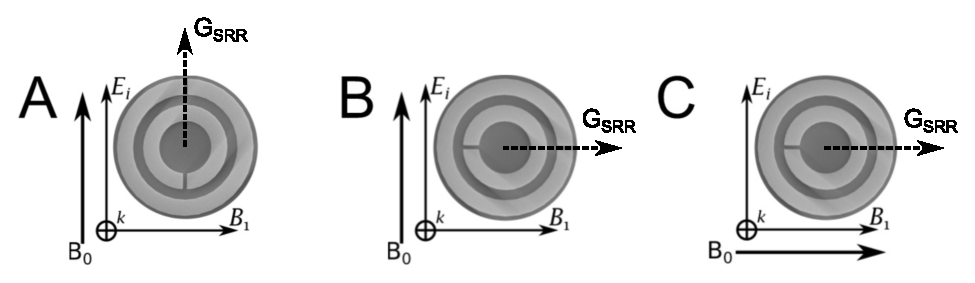
\includegraphics[width=0.8\textwidth]{Kapitel/Ch4-Images/Ch4-BeamPath.eps}
  \caption[THz TEM-wave Orientation Relative to SRR]{Illustrated is the THz TEM-wave orientation relative to the SRR geometry and $\vectu{B}{0}$. Shown is A) $\vectu{B}{1} \perp \vectu{B}{0}$ \& $\vectu{E}{i}||\vectu{G}{SRR}$ B) $\vectu{B}{1} \perp \vectu{B}{0}$ \& $\vectu{E}{i}\perp\vectu{G}{SRR}$ and C) $\vectu{B}{1} || \vectu{B}{0}$ \& $\vectu{E}{i}\perp\vectu{G}{SRR}$.}
  \label{ch4-fig:BeamGEO}
\end{figure}

The path was chosen such that the static magnetic field $\vectu{B}{0}$ was perpendicular to the direction of the THz wave propagation $\vect{k}$, illustrated in Fig.~\ref{ch4-fig:BeamGEO}. Hence, the magnetic flux density ($\vectu{B}{1}$) and electric field ($\vectu{E}{i}$) component of the THz radiation can be chosen parallel or perpendicular to the static magnetic field $\vectu{B}{0}$. This allowed three experiments with different THz electric and magnetic TEM-wave orientations relative to the SRR gaps ($\vectu{G}{SRR}$) and static magnetic field ($\vectu{B}{0}$) to be performed. These experiments are when the propagating $\vectu{B}{1}$ is 

\begin{enumerate}[label=(\Alph*)]
    \item $\vectu{B}{1} \perp \vectu{B}{0}$ \& $\vectu{E}{i}||\vectu{G}{SRR}$: perpendicular to the static magnetic field and the electric field is parallel to the SRR gaps. In this configuration, the SRRs resonance is inactive and only the EPR transition from the incident THz magnetic flux density can be observed. This configuration is named the ``No Coupling to SRR with EPR Transition'' mode. 
    \item $\vectu{B}{1} \perp \vectu{B}{0}$ \& $\vectu{E}{i}\perp\vectu{G}{SRR}$: perpendicular to the static magnetic field and the electric field is perpendicular across the SRR gaps. In this configuration, both the incident THz flux density and the coupled flux density from the SRR excite an EPR transition. This configuration is named the ``Coupling to SRR with EPR Transition'' mode.
    \item $\vectu{B}{1} || \vectu{B}{0}$ \& $\vectu{E}{i}\perp\vectu{G}{SRR}$: parallel to the static magnetic field and the electric field is perpendicular across the SRR gaps. In this configuration, no EPR transitions occur from the THz TEM-wave. However, the SRRs resonance is coupled with the electric field generating a $\vectu{B}{1}$ at the SRR geometry. This configuration is named the ``Coupling to SRR without EPR Transition'' mode.
\end{enumerate}


\section{Theory}
An analytical model of the experiment is derived to better understand the complex interactions of the EPR signal with the SRR meta-material. Typically, in antenna design one would choose only magnetic \cite{srrmodel} or electric \cite{Katsarakis04} excitation since magnetic and electric coupling counteract total mutual impedance. Because of this, to our knowledge, the use of both magnetic and electric coupling has not been employed in the literature and for antenna design. For antenna design, only one is necessary to properly describe the coupling of the SRR. \cite{Baena2005,DurnSindreu2012,Bojanic2014,Su2015} However, this is not the case when describing the SRRs in a magnetic resonance experiment. When modeling both the frequency dependence of the SRR and the frequency dependence of the magnetic resonance, both magnetic and electric coupling is needed due to non-zero magnetic field interactions (inductive) and electric field across the gap (capacitive) in the neighborhood of resonance. This is described in detail and the Mathematica (Wolfram Research, Champaign, Illinois; v.12.1) code can be found in Appendix~C.

Fundamentally, the FD-FT EPR experiment is the measurement of the change in the magnetic susceptibility of the sample as a function of frequency for a given static magnetic field. Therefore the experiment can be modeled as a continuous-wave experiment by defining the permeability as described in Eqn.~\ref{eq-2:permea} as a function of the magnetic susceptibility $\chi(\omega)$ of Eqn.~\ref{eq-2:chi}. For simplicity, the Lorentzian line-shape in the neighborhood of resonance of Eqn.~\ref{eq-2:chi} was used to mimic the feature at the effective $g$-value of 6. The Lorentzian line-shape reproduces the spectral features well and modeling the true line-shape here does not improve the understanding of the experiment. 

\noindent \paragraph*{Lossless transmission\-/line model with EPR sample.} A free-space lossless transmission\-/line representation includes a series inductance (L$_L$) with the value $\mu_0$ as $4 \pi \times 10^{-7}$ [H/m] and shunt capacitance (C$_L$) with the value of $\epsilon_0$ as $8.854 \times 10^{-12}$ [F/m]. \cite{ramo1984fields} Therefore, the characteristic impedance of the lossless transmission, defined as
\begin{equation}
    Z_0 = \sqrt{\frac{L_L}{C_L}} = \sqrt{\frac{\mu_0}{\epsilon_0}},
\end{equation}
has a free-space value of 376.7~$\Omega$ and assumes infinitely long propagation. 

As the THz electromagnetic wave interacts with the sample and the magnetic resonance condition is met, a change in the magnetic susceptibility occurs. Since our transmission-line model incorporates a sample, the free-space $\mu_0$ is replaced with $\mu_r(\omega)$ as defined in Eqs.~\ref{eq-2:permea} and \ref{eq-2:chi}. As the static magnetic field is swept, the trans-impedance of the wave is modified and the resulting intensity change is recorded.

\noindent \paragraph*{Coupled Resonant Circuit with EPR sample.} Since little mutual coupling occurs between single SRR geometries, it is sufficient to estimate the inductance of a single SRR and model a simplified transmission\-/line coupled system. The inductance of the SRR is estimated by the classic equation for the inductance of a loop of wire, such that 
\begin{equation}
    L_R(\omega) = \mu_r(\omega) a_r \left(\text{Log}\left[ \frac{8 a_r}{a_w} \right] -2\right),
\end{equation}
where $a_r$ is the effective radius of the loop, and $a_w$ is the radius of the wire. \cite{ramo1984fields} The capacitance of the SRR (C$_R$) can be estimated by the resonance equation $\omega_R^2 L_RC_R=1$, where $\omega_R$ is the resonant frequency of the SRR in radians/s. The resistance is chosen such that the $Q_0$-value matches the measured SRR $Q_0$-value. This is calculated by
\begin{equation}
    Q_0(\omega) = \frac{\omega_R L_R(\omega)}{R_R} \approx 10.
\end{equation}

\begin{figure*}[htp]
\centering
   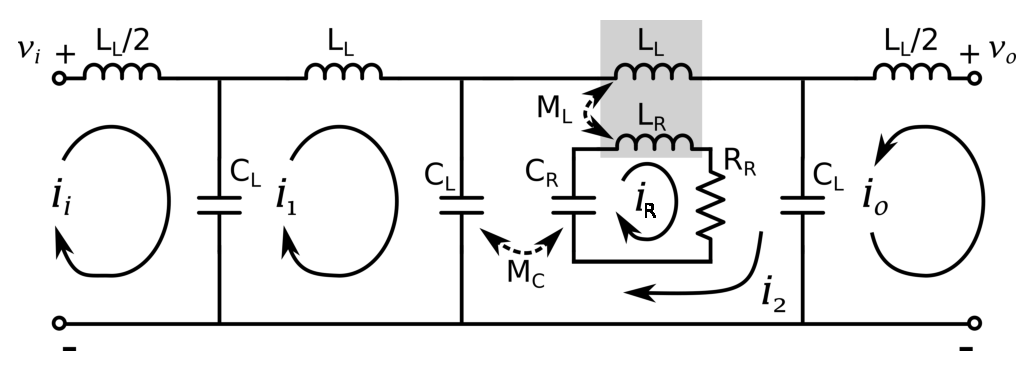
\includegraphics[width=\textwidth]{Kapitel/Ch3-Images/03-CircuitFig.eps}%
\caption[Transmission\-/line lumped circuit model.]{Transmission\-/line lumped circuit model used to describe the SRR coupling to a plane-wave excitation. Both mutual capacitance ($M_c$) and mutual inductance ($M_L$) are used to describe the circuit. Shown in grey is the region of the circuit where magnetic resonance occurs.}
  \label{ch3-fig:circuit}
\end{figure*}

Using a circuit model of a transmission line with a coupled resonant circuit, illustrated in Fig.~\ref{ch3-fig:circuit}, one can derive the current mesh equations. Such that
\begin{subequations}
\begin{eqnarray}
i(\omega L_L/2 - \frac{1}{\omega C_L}) \text{i}_i +  i\frac{1}{\omega C_L} \text{i}_1 &= v_i  \\
i\frac{1}{\omega C_L} (\text{i}_{i}+\text{i}_2) + i(\omega L_L - \frac{2}{\omega C_L}) \text{i}_{1} + \nonumber \\
 i \omega M_c \text{i}_R &= 0  \\
i\frac{1}{\omega C_L} (\text{i}_{1}-\text{i}_{o}) + i(\omega L_L - \frac{2}{\omega C_L}) \text{i}_{2} + \nonumber \\
i \omega (M_c - M_L) \text{i}_R &= 0  \\
i \frac{1}{\omega C_L} \text{i}_{2} + i(\omega L_L - \frac{2}{\omega C_L}) \text{i}_{o}  &= v_o  \\
i \omega (M_c) \text{i}_{1} + i \omega (M_L - M_c)\text{i}_2 + \qquad \nonumber \\ 
(R_R + i \omega L_R - i\frac{1}{\omega C_R}) \text{i}_R  &= 0
\end{eqnarray}\label{ch3-eq:lineareq}
\end{subequations}

\noindent 
where $v_i$ and $v_o$ is the input and output voltage and $i_i$ and $i_o$ is the input and output mesh currents, respectively, of the transmission-line model, while C$_R$ is the capacitance, L$_R$ is the inductance, and R$_R$ is the resistance of the SRR. The mesh currents $i_1$ and $i_2$ are indicated in Fig.~\ref{ch3-fig:circuit} within the transmission line and $i_R$ is the mesh current within the SRR. The mutual inductance ($M_L$) and mutual capacitance ($M_c$) are defined by the coupling coefficients, 
\begin{subequations}
\begin{eqnarray}
    M_c &= k_c \sqrt{C_R C_L}\quad \text{and} \\
    M_L &= k_L \sqrt{L_R L_L}.
\end{eqnarray}
\end{subequations}

The set of linear equations of Eqn.~\ref{ch3-eq:lineareq} are solved for the currents using Wolfram Mathematica.\footnote{It should be noted that L$_R$, L$_L$, $M_L$ are all functions of $\omega$ from the relationship with Eqn.~\ref{eq-2:permea}. This has been removed in the equations for better readability.} The relationship of the currents to the voltage is used to find the open-circuit forward trans-impedance, where
\begin{equation}
    Z_{21}(\omega) = \frac{v_o}{\text{i}_i} \Biggr\rvert_{\text{i}_o=0} =i \frac{(\omega L_L/2 - \frac{1}{\omega C_L}) \text{i}_o - \frac{1}{\omega C_L} \text{i}_2  }{\text{i}_i} \Biggr\rvert_{\text{i}_o=0}.
\end{equation}

To mimic the FD-FT THz EPR experiment, the open-circuit forward trans-impedance $Z_{21}(\omega)$ is evaluated at two EPR resonance frequencies $\omega_0$ from Eqn.~\ref{eq-2:permea} that are 5~GHz apart to produce two spectra for frequency division. These two frequencies in the transmission\-/line model represent the EPR resonance shift that occurs at two static magnetic fields as performed in the FD-FT EPR experiment. The ``resonance shift'' is a parameter that is varied step-wise from 1.0-2.0 to shift the spectrum between the energy range of 11-18~cm$^{-1}$. The transmission\-/line model division spectrum is calculated by, 
\begin{equation}
    S(\omega) = \frac{Z_{21}(\omega)\Bigr\rvert_{\omega_0 = \omega_a}}{Z_{21}(\omega)\Bigr\rvert_{\omega_0 = \omega_b}} - 1
\end{equation}
where $S(\omega)$ is the EPR signal and $\omega_a$ and $\omega_b$ are two EPR resonance frequencies representing the resonance shift due to a change in B$_0$. The pair of frequencies $\omega_a$ and $\omega_b$ are stepped across the energy range using a ``resonance shift'' parameter to mimic the change in the static magnetic field. In the experiment and this model, it is important to note that the SRR resonance energy (frequency) does not change when a static magnetic field is applied. Only the EPR transitions change the system as the magnetic susceptibility $\chi(\omega)$ is stepped through resonance.

\noindent \paragraph*{Strong- and Weak-Coupling Regimes}
When two resonant modes interact, the resulting frequency response greatly depends on the coupling of the two systems. Specifically, the $Q_0$-value of the SRR and the amplitude of the magnetic susceptibility $\chi(\omega)$. Two regimes exist as a continuum: weak-coupling and strong-coupling. 

The weak-coupling regime is characterized as only a perturbation as the EPR resonance passes through the SRR resonance when the static magnetic field is stepped. Weak-coupling interactions result in small shifts of the SRR frequency and $Q_0$-value. If one measures the change in these SRR parameters, a typical EPR experiment would be performed. The measured shift in SRR frequency and $Q_0$-value would correspond to dispersion and absorption signals, respectively. \cite{abragam1961, poole} Weak-coupling regime is desired for EPR experiments using meta-material surfaces.

However, as the concentration of the sample increases (increasing the magnetic susceptibility $\chi(\omega)$) or the $Q_0$-value increases, these systems can exhibit mode-splitting and anti-crossing features centered around the frequency of the SRR and the neighborhood of the EPR resonance. This regime, called strong-coupling, is intensified by resonant structures with large filling factors and can be likened to radiation damping. \cite{BloembergenRadDamp, BloomRadDamp, MeiboomRadDamp} One consequence of radiation damping is the second-order effect of the sample changing the current distributions of the resonator as it passes through resonance. Some qualitative understanding of a system with strong-coupling in the context of EPR has led to the understanding of this effect employing the two-coupled oscillator problem. \cite{SchneiderEPR,BOERO2013133,Scalari1323} Herein it is shown that the lumped-circuit transmission\-/line model approximates this interaction. 

\section{Results and Discussion}
The magnitude of the electric and magnetic field profile at the resonance frequency of the SRR (418~GHz) is shown in Figs.~\ref{ch3-fig:HFSS}A and ~\ref{ch3-fig:HFSS}B, respectively. The dotted line represents the cut plane plotted to the right. To better assess the EPR sensitivity of the SRR with a 100~$\mu$m sample, the THz magnetic field squared is plotted in Fig.~\ref{ch3-fig:HFSS}C along the axis of the SRR. The magnetic field squared is proportional to the EPR signal. In Fig.~\ref{ch3-fig:HFSS}, a dash-dot line is plotted at 24~$\mu$m where the area between the quartz substrate surface (0~$\mu$m) and 24~$\mu$m represents 90\% of the EPR signal.

\begin{figure}[htp]
\centering
  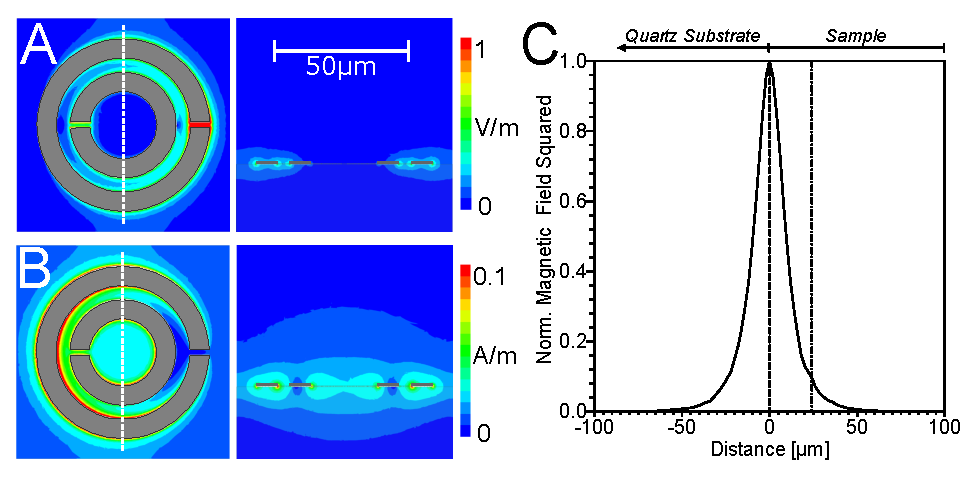
\includegraphics[width=0.9\textwidth]{Kapitel/Ch3-Images/02-AnsoftFields.eps}%
  \caption[Finite-element simulation solutions of SRR geometry.]{Finite-element modeling solutions plotting the magnitude of the THz A) electric and B) magnetic field profile of the SRR. A cut plane is shown as a dotted line. C) Simulated THz magnetic field profile squared (proportional to EPR signal) on the axis of the SRR. The plot starts from -100~$\mu$m into the quartz substrate and through the SRR until the depth of the sample at 100~$\mu$m. The dash-dot line shows that 90\% of the EPR signal originates from a depth of 24~$\mu$m.}
  \label{ch3-fig:HFSS}
\end{figure}

Shown in Fig.~\ref{ch3-fig:resonator} (dashed line) is the result of the measurement at a temperature of 2~K and in the absence of a static magnetic field. This absorbance was then normalized to compare to simulations. Simulations are shown in Fig.~\ref{ch3-fig:resonator} as a solid line. The absorption feature is associated with the lowest-order resonance mode of the SRRs. \cite{Katsarakis04} Without the sample, at an energy of 14.47 cm$^{-1}$, a pronounced absorbance with the full width at half maximum (FWHM) of 1.45 cm$^{-1}$ was observed. After the thin film of hemin is placed on top of the SRRs, a shift of the absorbance to lower energy of 13.97 cm$^{-1}$, accompanied by a slight narrowing of the FWHM to 0.87 cm$^{-1}$, was observed. The absorptive feature could be identified in the intensity spectrum (not shown). Using the FWHM, $Q_0$-values of 10 and 17 were measured for both the SRR without sample and the SRR with the hemin sample, respectively. Simulations show the SRRs resonance at 13.76 cm$^{-1}$ for SRRs with a sample. The frequency deviation of the simulation from the experiment is only 1.5\%. The very good agreement is due to the high quality of the manufacturing of the SRRs. The $Q_0$-value of the simulated SRR is 42. The discrepancy is due to the unknown loss tangent of the hemin sample at THz frequencies.


\begin{figure}[htp]\centering
  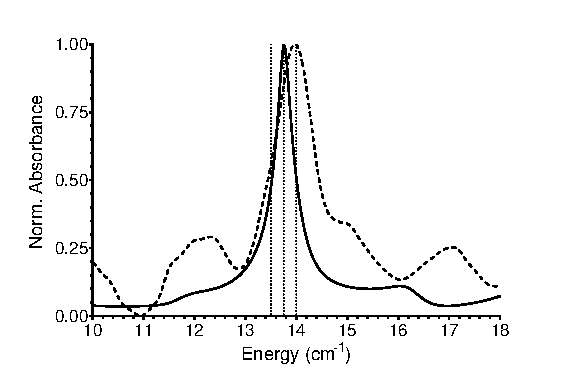
\includegraphics{Kapitel/Ch3-Images/03-SRR_Profile.eps}%
  \caption[Simulated and measured SRR resonance.]{Resonance condition of the SRR meta-material with 100~$\mu$m sample calculated using HFSS (solid) and measured (dashed) shown by plotting the normalized absorbance.}
  \label{ch3-fig:resonator}
\end{figure}

\begin{figure}[htbp]\centering
  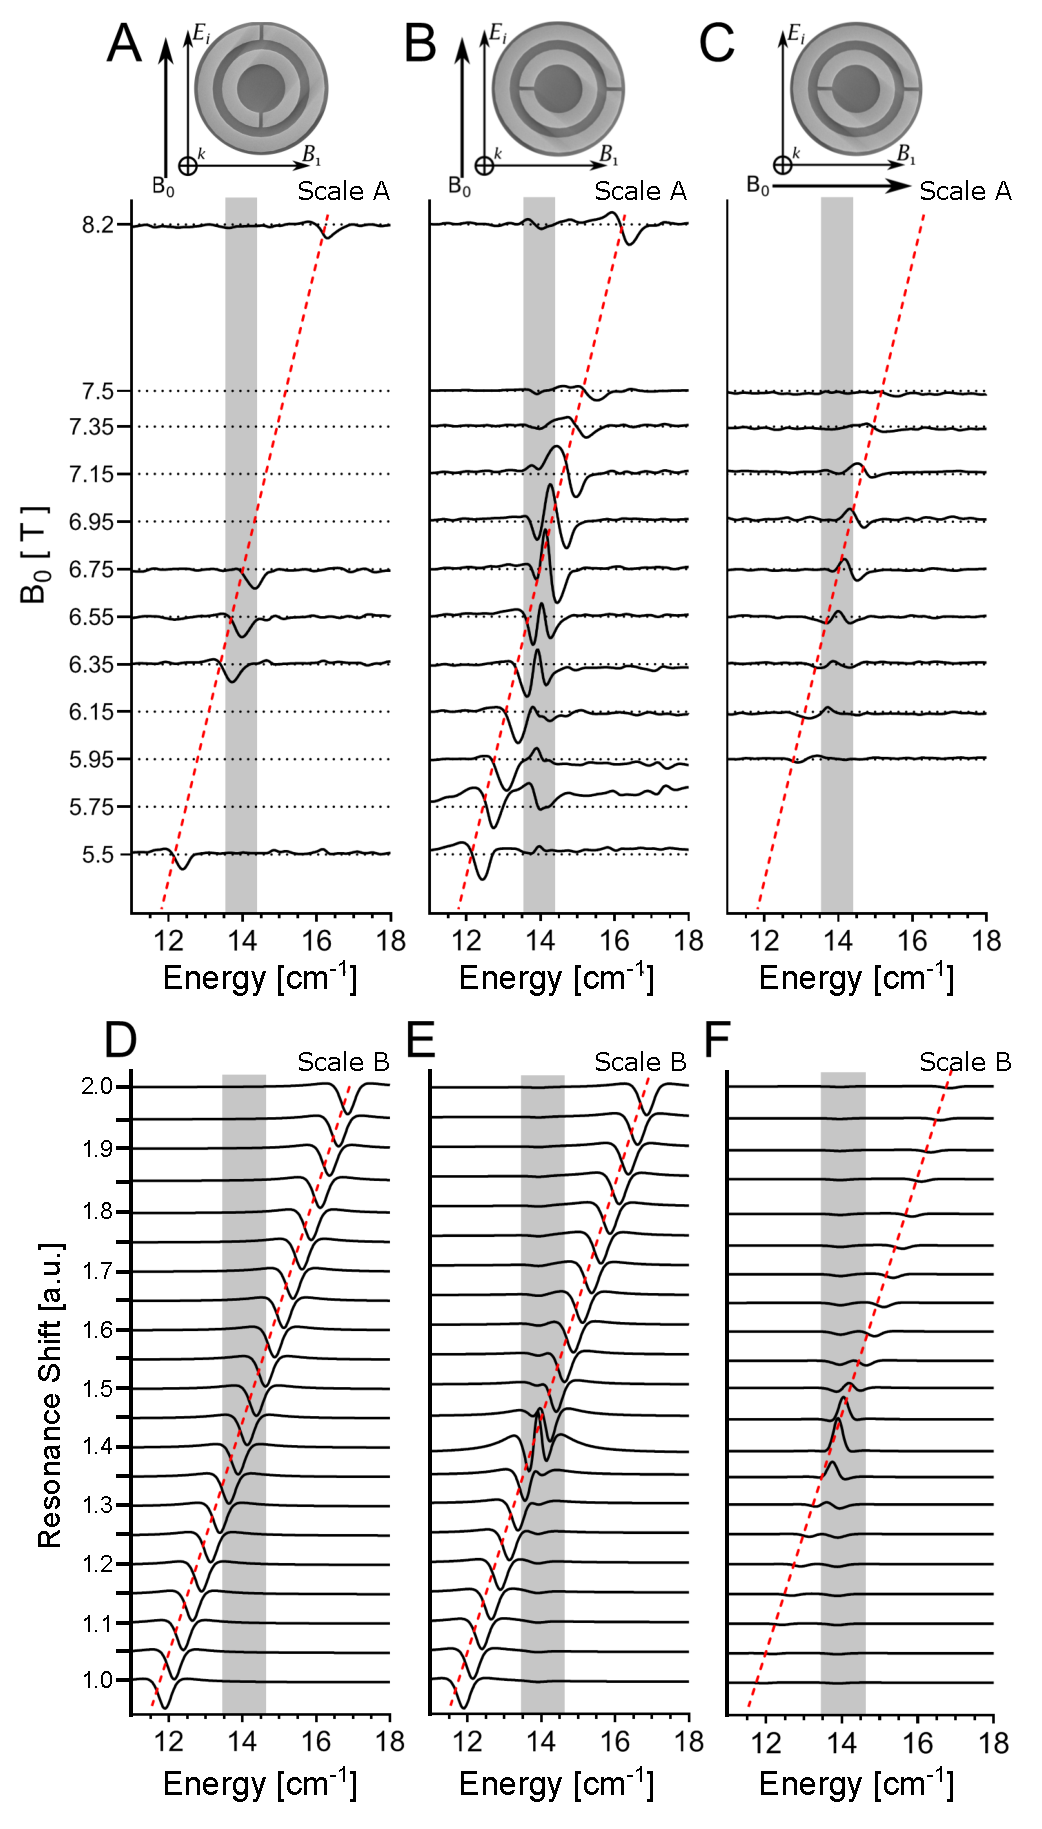
\includegraphics[width=0.7\textwidth]{Kapitel/Ch3-Images/HugeData.eps}%
  \caption[FD-FT EPR Data and Lumped-Circuit Model with SRRs]{Measured data and lumped-circuit model EPR signal interacting with the SRRs. The red dotted line indicates the calculated transition energy. The grey shaded area indicates the bandwidth of the SRRs with the sample. The SRRs are depicted by a single SRR. The direction of the static magnetic field $\vectu{B}{0}$ is shown compared to the THz radiation traveling wave normal to the SRRs, i.e the $\vect{k}$ vector goes into the paper, with $\mathbf{E}_i$ and $\mathbf{B}_1$ components indicated. The measurements in the three configurations are: A) No Coupling to SRR with EPR Transition, B) Coupling to SRR with EPR Transition, and C) Coupling to SRR without EPR Transition. The series is repeated using the lumped-circuit model in D-F.\label{ch3-fig:datacompare}}
\end{figure}

The EPR transition will only be observed for the magnetic flux density component of the THz radiation $\vectu{B}{1}$ perpendicular to the static magnetic field $\vectu{B}{0}$ ($\vectu{B}{1} \perp \vectu{B}{0}$). \cite{Nehrkorn15_PRL} Additionally, the resonance of the SRRs only couple to the THz radiation if the electric field is parallel to the gap of the rings of the SRRs ($\vectu{E}{i}\perp\vectu{G}{SRR}$). \cite{Katsarakis04} The results of a series of FD-FT EPR experiments can be found in Fig.~\ref{ch3-fig:datacompare}A-C and each measurement is described below. The spectra of Fig.~\ref{ch3-fig:datacompare}A-C are on the same scale (indicated as Scale A).

\noindent \paragraph*{No Coupling to SRR with EPR Transition.} In this configuration the feature at the effective $g$-value of 6 of high-spin Fe is observed with almost unchanged intensity over the measured field and frequency range, shown in Fig.~\ref{ch3-fig:datacompare}A. This data confirms the SRRs resonance was inactive since only the EPR transition was observed. 

\noindent \paragraph*{Coupling to SSR with EPR Transition.} Measured data, shown in Fig.~\ref{ch3-fig:datacompare}B, exhibited an increase in the EPR signal of hemin in the frequency range where the EPR line and the SRRs resonance overlap. Over this region, a complex interaction occurs where real and imaginary parts of the magnetic susceptibility $\chi(\omega)$ mix with the frequency-dependent effective $\mu(\omega)$ and $\epsilon(\omega)$ of the SRR.

\noindent \paragraph*{Coupling to SSR without EPR Transition.} In this experiment, $\vectu{B}{1}$ is parallel to $\vectu{B}{0}$ and, as such, EPR transitions should not be observed. However, in the region where the EPR line overlaps with the resonance of the SRRs a feature was observed, data are shown in Fig.~\ref{ch3-fig:datacompare}C. This can be rationalized by a magnetic flux density component $\vectu{B}{1}\perp\vectu{B}{0}$ that arises from the SRR geometry since $\vectu{E}{i}$ is perpendicular to the SRR gaps ($\vectu{G}{SRR}$). Hence, the observed EPR line was direct proof that an additional THz magnetic field was generated by the SRRs resonance. This configuration demonstrates the use of SRRs in resonance with THz radiation for resonant EPR detection at a single frequency. 

\noindent \paragraph*{Transmission\-/line model: Results.} Parameters to duplicate the FD-FT THz EPR experiments using the lumped-circuit transmission\-/line model of Fig.~\ref{ch3-fig:circuit} are shown in Table~\ref{ch3-table:lumpedparameters}. The inductance L$_r(\omega)$, capacitance C$_r$, and resistance R$_r$ needed to describe the SRR were found by calculating the inductance of a small loop (diameter 20~nm) and setting the capacitance to resonant at 13.9~cm$^{-1}$. The resistance chosen gives a $Q_0$-value of 10. The phenomenologically chosen EPR characteristics T$_1$, T$_2$, and $\gamma$ give a Lorentzian line of suitable width to approximate the experimentally observed feature at the effective $g$-value of 6 as measured in Fig.~\ref{ch3-fig:datacompare}A. 

\begin{table}[hbtp]
\centering
\caption{Parameters used for the lumped-circuit model characterization.}
\begin{tabular}{l|c}
\multicolumn{1}{l|}{Param.} & \multicolumn{1}{c}{Values} \\ \hline \hline
\multicolumn{1}{l|}{$L_r$} & \multicolumn{1}{c}{$29.76\times 10^{-15}$~H} \\
\rowcolor[rgb]{0.937,0.937,0.937}  
\multicolumn{1}{l|}{$C_r$} & \multicolumn{1}{c}{$4.89\times 10^{-12} $~F} \\
\multicolumn{1}{l|}{$R_r$} & \multicolumn{1}{c}{$0.008~\Omega$} \\
\rowcolor[rgb]{0.937,0.937,0.937}  
\multicolumn{1}{l|}{T$_1$} & \multicolumn{1}{c}{$4\times 10^{-9}$~s} \\
\multicolumn{1}{l|}{T$_2$} & \multicolumn{1}{c}{$0.1\times 10^{-9}$~s} \\
\rowcolor[rgb]{0.937,0.937,0.937}  
\multicolumn{1}{l|}{$\gamma$} & \multicolumn{1}{c}{$2.8$~MHz/G}
\end{tabular}\label{ch3-table:lumpedparameters}
\end{table}

The integral of the magnetic susceptibility $\chi(\omega)$ of Eqn.~\ref{eq-2:chi} was normalized and the parameters $g_f$ and $g_r$ were used for scaling. The parameters encompass the filling factor $\eta$ and number of spins for free-space and resonant signals, $g_f$ and $g_r$, respectively. From the right-hand side of Eqn.~\ref{eq-2:permea}, the substitution
\begin{equation}
    \eta \chi(\omega) =
    \begin{cases}
      g_f \hat{\chi}(\omega), & \text{for free-space}\ L_L(\omega) \\
      g_r \hat{\chi}(\omega), & \text{for resonator}\ L_R(\omega)
    \end{cases}
\end{equation}\label{etagfgr}
where $\hat{\chi}(\omega)$ is the normalized magnetic susceptibility. Therefore, adjusting  $g_f$ and $g_r$ affects the EPR signal intensity by scaling $\mu_r(\omega)$ in L$_L(\omega)$ and L$_r(\omega)$, respectively, in the lumped-circuit transmission\-/line model. The parameters $g_f$ and $g_r$ can be visualized in the illustration of Fig.~\ref{ch3-fig:effetachi}. The parameter $g_f$ represents the whole sample that is excited by the THz plane-wave traveling through the sample, illustrated as the blue hatch in Fig.~\ref{ch3-fig:effetachi}A. The parameter $g_r$ represents only the sample that is excited by the SRRs, illustrated as the blue hatch in Fig.~\ref{ch3-fig:effetachi}B. When both the EPR transitions and SRR are coupled ($\vectu{B}{1}\perp\vectu{B}{0}$ and $\vectu{E}{i}\perp\vectu{G}{SRR}$) the linear combination of Figs.~\ref{ch3-fig:effetachi}A and \ref{ch3-fig:effetachi}B is excited. The spectra of Figs.~\ref{ch3-fig:datacompare}D-F use the same $g_f$ and $g_r$ parameters and, therefore, are on the same scale (indicated as Scale B). The parameters used to characterize the coupling and EPR signal for the lumped-circuit model are found in Table~\ref{ch3-table:parameters}.

\begin{figure}[htbp]\centering
  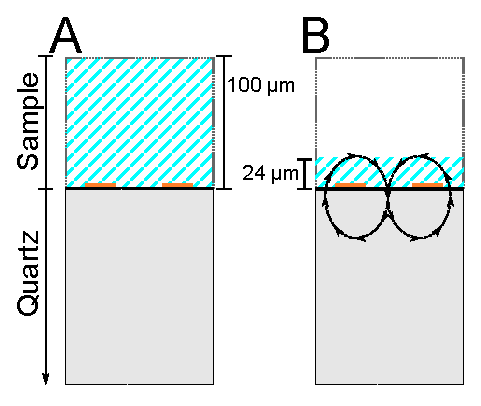
\includegraphics{Kapitel/Ch3-Images/Ch4-SampleVisualization.eps}%
  \caption[Illustration of the excited sample volumes.]{An illustration showing the effective volume for A) the experiment without SRRs coupling and B) the experiment with only SRRs coupling. Here the hatched blue area is the volume of spins and the grey area is the quartz substrate. The THz magnetic field vectors (dashed arrows) are illustrated for the SRR geometry (orange).
  \label{ch3-fig:effetachi}}
\end{figure}

In the calculation, coupling was adjusted using the inductive $k_L$ and capacitive $k_c$ coupling constants and fit to the data of Fig.~\ref{ch3-fig:datacompare}B. It is noted that the coupling constants are not unique. Nevertheless, one interesting outcome of this model is the ratio of the amplitude parameters $g_f$ and $g_r$. A factor of 4.7 is realized for the apparent intensity of the EPR spins in the 24~$\mu$m region. This result is consistent with the THz magnetic field squared profile of Fig.~\ref{ch3-fig:HFSS}C showing a factor of 4.2 for the sample to active-region ratio compared to Fig.~\ref{ch3-fig:HFSS}B. This is reproduced in Figs.~\ref{ch3-fig:HFSS}D and ~\ref{ch3-fig:HFSS}F.

\begin{table}[htp]
\centering
\caption[Parameters used for the EPR characterization using the lumped-circuit model.]{Parameters used for the EPR characterization using the lumped-circuit model. The following configurations of A) $\vectu{B}{1}\!\perp\!\vectu{B}{0}$ \& $\vectu{E}{i}||\vectu{G}{SRR}$, B) $\vectu{B}{1}\!\perp\!\vectu{B}{0}$ \& $\vectu{E}{i}\!\perp\!\vectu{G}{SRR}$, and C) $\vectu{B}{1}||\vectu{B}{0}$ \& $\vectu{E}{i}\!\perp\!\vectu{G}{SRR}$ are shown. }
\begin{tabular}{ll}
%\multicolumn{1}{r}{}&{$\vectu{B}{1}\!\perp\!\vectu{B}{0}$ \& $\vectu{E}{i}||\vectu{G}{SRR}$} \\
\multicolumn{1}{r}{\textbf{{\Large A.}}}&{} \\
\multicolumn{1}{l|}{} & \multicolumn{1}{c}{Values} \\ \hline \hline
\multicolumn{1}{l|}{$g_f$} & \multicolumn{1}{c}{$10\times 10^{-6}$} \\
\rowcolor[rgb]{0.937,0.937,0.937}  
\multicolumn{1}{l|}{$g_r$} & \multicolumn{1}{c}{$47\times 10^{-6}$} \\
\multicolumn{1}{l|}{$k_c$} & \multicolumn{1}{c}{0} \\
\rowcolor[rgb]{0.937,0.937,0.937}  
\multicolumn{1}{l|}{$k_L$} & \multicolumn{1}{c}{0.065}\\
\end{tabular}\hspace{1em}
\begin{tabular}{ll}
%\multicolumn{1}{r}{}&{$\vectu{B}{1}\!\perp\!\vectu{B}{0}$ \& $\vectu{E}{i}\!\perp\!\vectu{G}{SRR}$} \\
\multicolumn{1}{r}{\textbf{{\Large B.}}}&{} \\
\multicolumn{1}{l|}{} & \multicolumn{1}{c}{Values} \\ \hline\hline
\multicolumn{1}{l|}{$g_f$} & \multicolumn{1}{c}{$10\times 10^{-6}$} \\
\rowcolor[rgb]{0.937,0.937,0.937}  
\multicolumn{1}{l|}{$g_r$} & \multicolumn{1}{c}{$47\times 10^{-6}$} \\
\multicolumn{1}{l|}{$k_c$} & \multicolumn{1}{c}{0.255} \\
\rowcolor[rgb]{0.937,0.937,0.937}  
\multicolumn{1}{l|}{$k_L$} & \multicolumn{1}{c}{0.065}
\end{tabular}\hspace{1em}
\begin{tabular}{ll}
%\multicolumn{1}{r}{}&{$\vectu{B}{1}||\vectu{B}{0}$ \& $\vectu{E}{i}\!\perp\!\vectu{G}{SRR}$} \\
\multicolumn{1}{r}{\textbf{{\Large C.}}}&{} \\
\multicolumn{1}{l|}{} & \multicolumn{1}{c}{Values} \\ \hline\hline
\multicolumn{1}{l|}{$g_f$} & \multicolumn{1}{c}{0} \\
\rowcolor[rgb]{0.937,0.937,0.937}  
\multicolumn{1}{l|}{$g_r$} & \multicolumn{1}{c}{$47\times 10^{-6}$} \\
\multicolumn{1}{l|}{$k_c$} & \multicolumn{1}{c}{0.255} \\
\rowcolor[rgb]{0.937,0.937,0.937}  
\multicolumn{1}{l|}{$k_L$} & \multicolumn{1}{c}{0.065} 
\end{tabular}\label{ch3-table:parameters}
\end{table}

Using the transmission\-/line model, the ``EPR Transition without SRR Coupling'' mode is realized by setting the coupling constant $k_c$ to zero, illustrated in Fig.~\ref{ch3-fig:datacompare}D and with parameters reproduced in Table~\ref{ch3-table:parameters}A. The magnetic coupling constant $k_L$ is not set to zero because there is some component of the THz magnetic field that generates a small current on the SRR as shown by the simulations of the surface currents in Fig.~\ref{ch3-fig:surfacecurrent}. The scattering magnetic field from the surface currents generated by magnetic coupling does not perturb the EPR transitions from the THz TEM-wave. The transmission\-/line model results of the ``EPR Transition without SRR Coupling'' mode are shown in Fig.~\ref{ch3-fig:datacompare}D.

\begin{figure}[htbp]\centering
  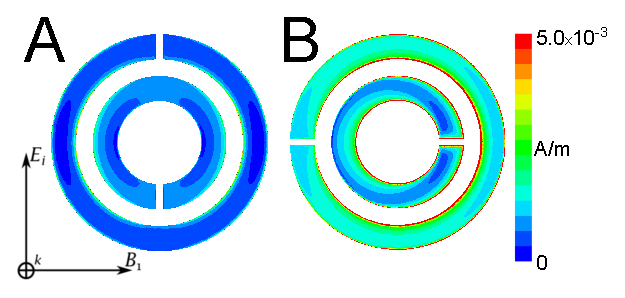
\includegraphics{Kapitel/Ch3-Images/SurfaceCurrent-THz.eps}%
  \caption[Simulation of the surface currents for SRR coupling.]{Simulation of the surface currents for SRR coupling. The plane wave used to excite both profiles is shown on the left. A) When the SRR is not coupled to the THz TEM-wave ($\vectu{E}{i}||\vectu{G}{SRR}$) there exist surface currents from inductive coupling, $k_L$. B) When the SRR is coupled to the THz TEM-wave ($\vectu{E}{i}\perp\vectu{G}{SRR}$) surface currents are generated primarily by capacitive coupling $k_c$, yet inductive coupling $k_L$ still exists.} \label{ch3-fig:surfacecurrent}
\end{figure}


In the ``Coupling to SRR with EPR Transition'' mode, the EPR transitions occur ($g_f$ is non-zero) and the SRRs are coupled. Using the transmission\-/line model, the response of the coupled resonance shown in Fig.~\ref{ch3-fig:datacompare}B is duplicated. Data is plotted in Fig.~\ref{ch3-fig:datacompare}E and with parameters reproduced in Table~\ref{ch3-table:parameters}B. The change in the spectral shape shown in Figs.~\ref{ch3-fig:datacompare}B and \ref{ch3-fig:datacompare}E can be interpreted as a phase shift between the EPR transition and the frequency-dependent effective $\mu(\omega)$ and $\epsilon(\omega)$ of the SRR. The phase shift is directly related to the capacitive (electric) and inductive (magnetic) coupling, $k_c$ and $k_L$, respectively. The spectral shape cannot be reproduced without the small magnetic coupling $k_L$. The magnetic coupling is enhanced at resonance and both electric and magnetic coupling was required to fit the model to the experiment.

In the ``Coupling to SRR without EPR Transition'' mode, the EPR transitions do not occur ($g_f$ is zero), but the SRRs are coupled to the THz TEM-wave. The effect of the coupled resonance is duplicated in the calculated data using the lumped-circuit impedance, shown in Fig.~\ref{ch3-fig:datacompare}B and with parameters reproduced in Table~\ref{ch3-table:parameters}C. 

At the SRR resonance, a magnetic resonance feature around 14~cm$^{-1}$ can be seen that does not shift with the magnetic field, shown clearly in Fig.~\ref{ch3-fig:datacompare}B at a static magnetic field of 8.2~T. This feature is also shown in calculated data in Figs.~\ref{ch3-fig:datacompare}E and ~\ref{ch3-fig:datacompare}F. This is an interesting feature that, at the time, was thought to be noise, since any EPR transition should follow the linear step of the magnetic field. However, the enhancement provided by the SRRs increases sensitivity. This enhancement of the ``tails'' of the EPR line is detectable even at the edge of the neighborhood of resonance. This effect can be enhanced by approaching the strong-coupling domain as demonstrated with the transmission\-/line model.

\noindent \paragraph*{Transmission\-/line model: Weak- and Strong Regime.} The transmission\-/line model indicates that the spin system is in a weak-coupling regime, illustrated in Fig.~\ref{ch3-fig:strong-weak}. Here the solid line represents the frequency shift using the parameters in Table.~\ref{ch3-table:parameters}C. A weak-coupling frequency perturbation is apparent at a simulated ``resonance shift'' of 1.4 (black dotted). The perturbation is compared to a constant SRR frequency of 14~cm$^{-1}$ (approximately 420~GHz), represented as a dashed line. As the concentration increases, the magnetic susceptibility $\chi(\omega)$ increases and a non-linear effect occurs between the EPR transition and the resonant frequency of the SRR. This effect is the strong-coupling regime. This is characterized by two resonances ($\CIRCLE$ and $\blacksquare$) interacting and creating an anti-crossing profile. A third resonance, denoted by the symbol $\hexagon$ occurs as the linear shift crossing displaying the onset of strong-coupling. In Fig.~\ref{ch3-fig:strong-weak}, $g_f$ was set to zero and $g_r$ was increased 100 fold to create the strong-coupling regime compared to the model used to describe the experiment of Fig.~\ref{ch3-fig:datacompare}F and Table~\ref{ch3-table:parameters}C. In practice, the increased in $g_r$ by 100 fold is equivalent to increasing the sample concentration by 100.

\begin{figure}[htp]\centering
  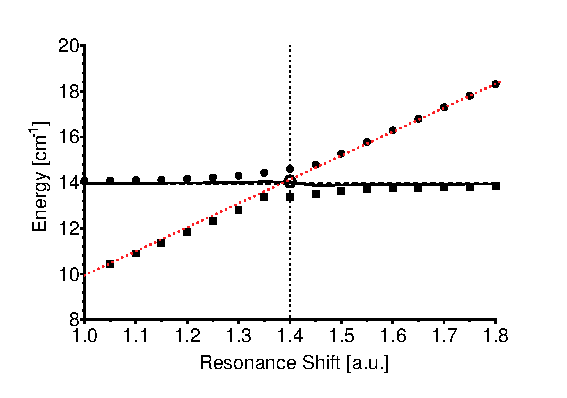
\includegraphics{Kapitel/Ch3-Images/08-RadiationDampening.eps}%
  \caption[Calculated weak- and strong-coupling regime using the analytical model.]{Using the lumped-circuit transmission\-/line model of Fig.~\ref{ch3-fig:circuit}, a weak- and strong-coupling plot can be obtained. Shown alongside is constant microwave energy (approximately 14~cm$^{-1}$; dashed). The crossover point is illustrated as a dotted line and represents an SRR resonance at 1.4. The weak-coupling regime is produced by the parameters in Table~\ref{ch3-table:parameters}C and is plotted as a black solid line. The symbols $\hexagon$, $\CIRCLE$, and $\blacksquare$ represent the frequencies in the strong-coupling regime, while the red dashed line represents the linear shift of the EPR signal as the static magnetic field is shifted.}\label{ch3-fig:strong-weak}
\end{figure}

\section{Conclusions and Outlook}
We have simulated and experimentally verified SRRs structures for measuring thin films with very high-frequency (3.34-33.36~cm$^{-1}$; THz-bandgap) EPR. The very good agreement between finite-element modeling simulations and the fabricated SRRs allowed us to investigate the interaction of the SRRs with the EPR line of a high-spin system. Our experiments revealed an increased EPR intensity by a factor of approximately 4 for an effective sample depth of 24~$\mu$m when the SRRs are employed as a surface resonator. Results were further confirmed using a lumped-circuit lossless transmission\-/line model which incorporates both magnetic and electric field coupling. The lumped-circuit model provides a unique way to study the interaction of spin-ensembles with meta-materials as the EPR transitions are swept through resonance. From first-principles, the EPR transitions have been included in lumped-circuit model permeability $\chi(\omega)$ which is then ``detected'' by the change in the trans-impedance of the coupled system.

Unlike meta-material literature for antennas, both magnetic and electric field coupling was required to match the experimental data. When designing a meta-material based antenna, the inductive coupling and capacitive coupling reduce the total coupling over a finite frequency range and provide only a bulk frequency-dependent effective $\mu(\omega)$ and $\epsilon(\omega)$. However, when the SRR is used as a surface resonator for EPR and is covered with a sample, the inductance L$_L(\omega)$ and mutual inductance $M_L(\omega)$ become a function of the EPR signal. Therefore, inductive coupling is not only a parameter for coupling but is a function of the EPR signal. Conversely, the electric field mutual capacitance $M_C$ does not vary with EPR magnetic resonance. This shift in inductive coupling in the neighborhood of EPR resonance contributes considerably to the shape of the measured signal.

The lumped-circuit transmission\-/line model gives us a good representation of meta-material enhanced FD-FT THz EPR experiment to optimize the SRR geometry for the study of diluted samples in thin films. For example, one could perform multi-frequency high-field EPR experiments. \cite{KRZYSTEK2006,Telser2014} Such multi-frequency high-field EPR experiments would require several meta-material resonant discs to be fabricated with resonances at multiple frequencies. A series of SRRs could be used to obtain broadband information allowing for the study of dilute protein samples.

The understanding presented here provides a framework to design more complicated meta-material unit structures. By changing the geometry of the unit structure from an SRR, the use of meta-materials can be tuned for further EPR spectroscopy enhancement. \cite{ZhangMetasurfaces}


{\renewcommand{\bibsection}{\clearpage\section*{\bibname}\markboth{\bibname}{\bibname}}
\renewcommand{\bibname}{CHAPTER 4. REFERENCES}
\bibliographystyle{elsarticle-num}
\bibliography{Kapitel/Ch4-References}
}
\chapter[Self-Resonant Micro-Helix at X-band]{Self-Resonant Micro-Helix for nano-Liter Volume Single-Crystals at X-band.\blfootnote{A significant portion of this chapter is from J.~W.~Sidabras, J.~Duan, M.~Winkler, T.~Happe,  R.~Hussein, A.~Zouni, D.~Suter, A.~Schnegg, W.~Lubitz, E.~J.~Reijerse, Sci. Adv., \textit{under review}.}}

For typical EPR experiments on proteins, a frozen solution of 0.1-1~mM concentration is prepared and placed in a microwave cavity. Standard sample volumes at X-band (nominally 9.5~GHz) are in the 200~$\mu$L range. However, frozen solution EPR experiments only allow the determination of the principal values of magnetic interactions at an active site, and thus provide only a limited view of the electronic structure. \cite{schweiger2001principles, goldfarb2018epr}

To resolve the full tensor magnetic interaction parameters, such as \textit{g}-, zero field, hyperfine-, and, for nuclei with $I>1/2$, quadrupole-tensors, single-crystal EPR experiments must be performed. In combination with X-ray crystallography, the magnetic-interaction tensors obtained with EPR experiments can be directly related to the protein geometry in order to help identify and better understand the catalytic mechanism of the enzyme. \cite{Bowman2016, NiFeRev2007} Despite its usefulness, single-crystal EPR is rarely applied to protein systems due to challenges in growing crystals of sufficient quality and volume for these experiments. Many protein crystals used in X-ray crystallography are of dimensions in the 50--300~$\mu$m range and, as such, are too small to be studied using commercial EPR instrumentation. Crystallization methods, such as macroseeding,\cite{macroseeding} have the potential to increase the volume of the crystals, but such techniques are difficult to implement. 

Currently, volume-limited crystals can only be studied using high-frequency EPR in a single-mode\cite{Hofbauer6623}, or, for continuous-wave experiments, Fabry-P\'{e}rot\cite{Klette94GHzPSI} resonators at W-band (94~GHz) or higher. Such high-frequency EPR spectrometers are not widely available and high-frequency conditions are usually unfavorable for advanced pulse experiments such as Electron Spin Echo Envelope Modulation (ESEEM) or Hyperfine Sub-level Correlation (HYSCORE) spectroscopies. \cite{pulseseq}

Unlike nuclear magnetic resonance (NMR), where all nuclei are excited and contribute to the NMR signal, hyperfine spectroscopy experiments, such as ESEEM, HYSCORE, and electron nuclear double resonance (ENDOR), probe only the nuclei that are magnetically coupled to the paramagnetic center. Extending these experiments to single crystals not only provides the magnitude of the hyperfine- and quadrupole-tensors of ligand nuclear spins that interact with the paramagnetic centers, but also the associated angles relative to the active site of an enzyme. Such interacting nuclei are either naturally abundant, such as $^1$H and $^{14}$N, or the catalytic cofactors can be enriched with nuclei such as $^2$H, $^{13}$C, $^{15}$N, and $^{57}$Fe, for further analysis of magnetic interaction tensors with respect to the first ligand-sphere. Furthermore, the same interaction tensors can be calculated from the molecular structure using quantum chemical calculations. \cite{NEESE2003125} These experimentally determined spectroscopic parameters can, therefore, be used to verify the adequacy of the level of theory which, in turn, gives confidence to the predicted electronic and geometric structure of the involved intermediates and transition-states in the whole catalytic cycle. The groundwork for understanding the inner workings of enzymes lies in collecting as much accurate spectroscopic information as possible, including other spectroscopic and structural methods (optical and vibrational spectroscopy, M{\"o}{\ss}bauer, X-ray spectroscopy, and diffraction). Every experiment contributes to the total picture and ultimately leads to a fundamental understanding of the catalytic mechanism of these enzymes.

To improve the sensitivity for studying single crystals using EPR on readily available spectrometers, typically at X-band, one must abandon the microwave cavity design and move to small-volume resonators based on lumped-circuits in the microwave frequency range. This allows the reduction of the sample volume by one order of magnitude, from 200~$\mu$L to 20~$\mu$L using a loop-gap resonator. \cite{hydehoff} Further reductions can be achieved by incorporating materials with a high dielectric constant in a standard resonator to reduce the active volume down to 1~$\mu$L. \cite{dielectricReson1, dielectricReson2} For protein single-crystals one must reduce the volume even further (less than 0.03~$\mu$L), which requires radical new approaches.

\begin{figure*}[htbp]
\centering
 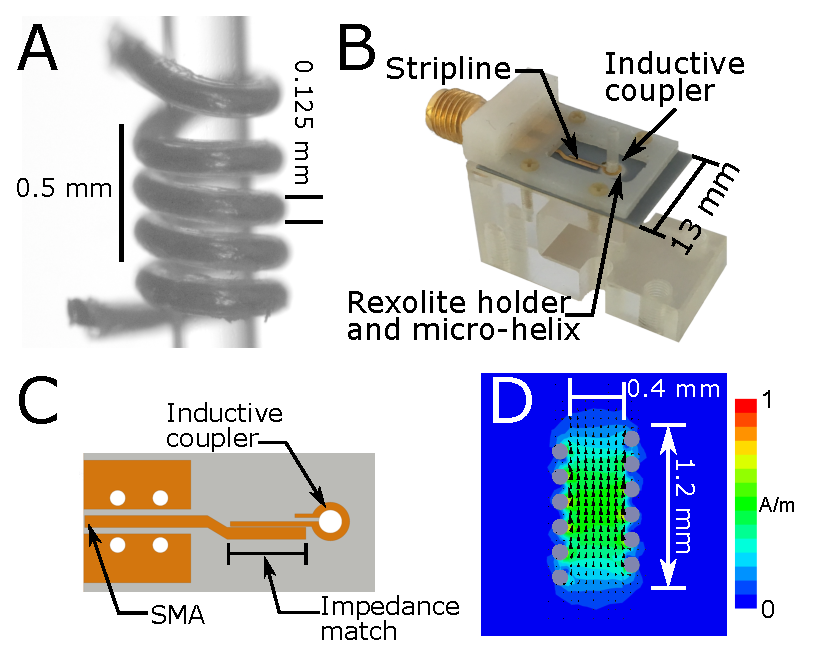
\includegraphics{Kapitel/Ch4-Images/01-MicroHelixHolder_Big2.eps}
 \caption[The self-resonant micro-helix.]{ The self-resonant micro-helix. A) A fabricated five-turn micro-helix wrapped around a 0.4~mm outer diameter capillary. During fabrication, the micro-helix is tightly wound around a 0.4~mm drill-bit and glued inside a Rexolite cylinder. The drill-bit is removed and the glue is allowed to dry for several days. The micro-helix assembly is placed in B) a coupling and support assembly, which includes a planar micro-coupler. C) The planar micro-coupler consists of a stripline impedance match to an inductive coupling loop. D) Finite-element modeling simulations of the microwave magnetic field, normalized to input power, at 9.5~GHz show an active region of good magnetic field homogeneity over a 0.8~mm height. The measured microwave magnetic field of 3.2 G/W$^{1/2}$ corresponds to a 20~ns $\pi$/2 pulse at approximately 20~mW. Dimensions of the micro-helix, where the self-resonance is determined by the capacitance formed between each turn and the inductance of the windings, are shown. The frequency can be tuned during fabrication by the number of turns, the pitch of the turns, or the inner diameter. The microwave characteristics of the fabricated micro-helix can be found in Table~\ref{table:chars}.}
 \label{fig:fabricated}
\end{figure*}

Herein, we combine the concept of a self-resonant micro-helix, shown in Fig.~\ref{fig:fabricated}A with that of a planar micro-coupler. The coupling structure on the printed-circuit board is a resonant structure which drives the self-resonant micro-helix placed in the center of the coupling loop\cite{coupling2016}, shown in Fig.~\ref{fig:fabricated}B. The micro-helix geometry offers significant advantages, in that, the microwave field homogeneity is strongly improved along with volume sensitivity for small samples, the microwave characteristics are optimal for pulse and continuous-wave experiments with need for very little microwave power, and the micro-helix assembly is easily matched and tuned over a variety of samples and temperatures.

\paragraph{Single-crystal EPR for metallo-enzyme research.}
For hydrogenases, specifically [NiFe]-hydrogenase, the single-crystal EPR strategy has been very successful. \cite{NiFe1996,NiFe2000, NiFe2003, NiFeRev2007} The active site of this enzyme harbors a [NiFe] binuclear cluster in which the iron carries two cyanide (CN$^-$) and one carbonmonoxide (CO) ligand. The metals are bridged by two cysteine thiols and the nickel center is further coordinated by two cysteine thiolate side groups. The paramagnetic states all originate from the nickel center, while the iron center remains Fe(II) during the catalytic cycle. \cite{lubitzhyd} The open-coordination site between the two metals can be occupied by an oxygen species leading to the inactive oxidized states or a hydride, which is the key intermediate in the catalytic cycle. \cite{NiFeRev2007} For all these species the $g$-tensor magnitude and orientation was determined and analyzed in terms of ligand-field theory and verified using quantum chemical calculations providing a fundamental insight into the electronic structure and the dependence on the first ligand-sphere. \cite{Ping2005, Gasteljp0573902, NiFeRev2007, LubitzNiFe2016} The [NiFe]-hydrogenase crystals in these studies were relatively large (2 $\times$ 0.5 $\times$ 0.5~mm$^3$) enabling measurements in standard X-band probe-heads with measuring time of 2-3 hours per angle, stepping over 180 degrees. However, even with the large crystal volume, ESEEM and HYSCORE experiments on [NiFe]-hydrogenase were only published in frozen solution with volumes of 50-200~$\mu$L and experimental times upwards of 2 hours for each experiment. \cite{NiFeRev2007} 

Similar experiments were anticipated for [FeFe]-hydrogenase which has a much higher activity and exhibits a different catalytic mechanism compared to [NiFe]-hydrogenase. Unfortunately, the crystals obtained from [FeFe]-hydrogenase are much smaller than those available from [NiFe]-hydrogenase with dimensions less than 0.3~mm. Frozen solution EPR on [FeFe]-hydrogenase has provided a lot of information on the binuclear active-site, such as, the discovery of a nitrogen in the dithiolate bridge (ADT-ligand). \cite{B905841A} However, the full $g$-tensor and the hyperfine-tensor, including angular information, of the active site are still elusive. Therefore, there is continuing interest in developing EPR instrumentation, specifically micro-resonators, at 9.5 and 35~GHz, X- and Q-band, respectively, optimized for metallo-enzyme research. Furthermore, other potentially interesting proteins (CODH\cite{C5CS00182J}, MMO\cite{Hoffman2014rev}, Rieske\cite{FERRARO2005175} and other Fe-S cluster containing proteins\cite{FeSClustersReview}) are rarely studied in single crystals, and doing so would contain a wealth of information on the electronic structure and enzymatic function. 

In this chapter, the design and implementation of a micro-helix is outlined. Experimental and simulated comparisons of the micro-helix geometry to commercially available and state-of-the-art resonator designs is presented. In order to further test the micro-helix geometry two experiments are performed on photosystem II tyrosine D radical: a 85~nL frozen solution and 0.3 $\times$ 0.18 $\times$ 0.18 mm$^3$ single crystal. These data demonstrate the utility of the micro-helix in studying protein single-crystals at volumes relevant for X-ray crystallography and provide a benchmark for future work.


\section{Methods}
All micro-helix and planar-coupling designs were modeled in the commercially available finite-element modeling program Ansys Electronics Desktop with HFSS (High Frequency Structure Simulator; v. 19.1) using driven mode. In driven mode, Ansys HFSS requires a coupling structure and mimics the output of a network analyzer. All designs are matched to 50~$\Omega$ with an S$_{11} < -35$~dB. Frequency and $Q$-values (-3~dB) are read directly from a simulated S$_{11}$-plot and $Q_0$-values are calculated by the known equation $Q=Q_0/(1+\beta$), where $\beta$ is the reflection coefficient at the frequency of resonance ($\beta=1$ for critically coupled). EPR signal intensity and resonator efficiency values (mT/W$^{1/2}$) were calculated using Ansys HFSS \cite{misrabook} and tabulated. EPR experimental comparisons were performed on an Elexsys E580 X-band bridge by Bruker Biospin. Four resonators are used for this comparison. The Bruker Biospin i) dielectric ER4118X-MD-5W1 (MD5W1) resonator and ii) LGR ER4118X-MS-3W1 (MS3; split-ring) resonators are used as comparisons with known commercial resonator geometries. Two $\Omega$-shaped 0.5~mm inner diameter PMR resonators are also tested. The first uses iii) Rogers 6010LM (RO6010LM printed-circuit board; Rogers Corp, Chandler, AZ, USA) substrate per Ref.~[5.\kern-0.4em\citenum{suter2015}] and one with (iv) sapphire substrate. The sapphire substrate was fabricated by Technical University Ilmenau (Ilmenau, Germany). Both PMR geometries have a 0.5~mm hole through the substrate. Resonator characteristics are found in Table~\ref{table:chars}. 

The continuous-wave EPR experiment measures the sample using a constant microwave power incident on the sample and slowly sweeping a quasi-static magnetic field through the resonance condition, $\nu =\gamma B_0$. Where $\nu$ is the operating frequency (nominally 9.5~GHz for X-band), $\gamma$ the the gyromagnetic ratio of the spin system ($\gamma = 2.8$~MHz/G for a free electron), and $B_0$ is the quasi-static magnetic field. The magnetic field is modulated, typically at 100~kHz, and collected using a phase-sensitive detector. \cite{weil2007electron} Continuous-wave is the standard EPR experiment. With modern digital signal processing and fast analog to digital converters, the continuous-wave experiment has recently been improved upon. The non-adiabatic rapid scan (NARS) \cite{KITTELL2011228, KITTELL201251, KITTELL201568, Hyde2013MDIFF, YU201558} and adiabatic rapid scan (RS) \cite{JOSHI200544,TSEITLIN200948, MITCHELL2012221, RScompare,MOSER2017} methods collect real and imaginary, pure-absorption and pure-dispersion, EPR spectra using fast quasi-static magnetic field or microwave frequency sweeps without the need for a phase-sensitive detector. Both rapid scan data can be pseudo-modulated to the conventional first-derivative EPR spectrum using a moving difference (MDIFF) pseudo-modulation. \cite{Hyde2013MDIFF} The non-adiabatic rapid scan (NARS) experiment uses a field sweep fast enough to overcome $1/f$ noise but remain in a thermal equilibrium, while adiabatic rapid scan sweeps the field fast enough to cause passage. The advantage of non-adiabatic rapid scan is the signal-to-noise improvement of collecting pure-absorption EPR spectra, while adiabatic rapid scan can further improve the continuous-wave and NARS experiment by changing the effective microwave magnetic field at the sample. This allows for an increase of microwave power, and thus, increase in EPR signal for saturable signals. \cite{JOSHI200544} While the non-adiabatic rapid scan method can be implemented on commercial bridges with no hardware changes, it does require some technical expertise. \cite{MOSER2017} However, to perform adiabatic rapid scan experiments on protein samples, custom current drivers are needed to increase the swept field amplitude. For simplicity, in this work, we have implemented only non-adiabatic rapid scan. Other experimental parameters are as stated in the manuscript.

The field-swept two-pulse electron spin-echo (ESE) experiment uses a ${\pi/2\!-\!\tau\!-\!\pi}$ pulse sequence ($\pi$ is 80~ns) that results in an echo $\tau$ seconds, herein $\tau$ is 300~ns, after the $\pi$ pulse. The field is stepped and a whole spectrum is acquired. This is the standard pulse sequence to collect an EPR spectrum. \cite{schweiger2001principles} 

Two EPR signal parameters were calculated in order to compare different resonant structures: i) unsaturable signal represents the EPR intensity at a given incident power, while ii) saturable signal represents the EPR intensity at a given microwave magnetic field that approaches the limit of saturation, i.e. the maximum achievable signal (P$_{1/2}$). For pulse experiments, the saturable signal is proportional to the EPR echo intensity in a two-pulse electron spin-echo (ESE) experiment. A 0.4~mm outer diameter and 0.3~mm inner diameter quartz capillary (QSIL GmbH, Ilmenau, Germany) with a 0.2~mm$^3$ ice sample ($\epsilon_r=3.17-i0.0035$, Ref.~[5.\kern-0.4em\citenum{icedielectric}] ) was used in the simulations. The signal-to-noise ratio for measured data is calculated by the ratio of the acquired signal mean to the standard deviation of the noise voltage, defined by
\begin{equation}
 \text{SNR}=\frac{S_{p\!-\!p}}{2\sigma_{noise}}
\end{equation}
where $S_{p\!-\!p}/2$ is the mean value of the peak-to-peak (or peak for absorption spectra) signal, and $\sigma_{noise}$ is the standard deviation of the noise. \cite{schroeder2000astronomical, oppenheim1999discrete} The standard deviation of the noise is calculated using 200 points in an off-resonance region.

The micro-helix is fabricated by hand winding 5 to 8 turns of 0.125~mm diameter silver wire with Polytetrafluoroethylene (PTFE) coating (0.0255~mm thickness, total 0.18~mm diameter; Science Products, GmbH, Hofheim, Germany) around a 0.4~mm drill bit and placed inside a Rexolite cylinder (0.8~mm inner diameter and 1.2~mm outer diameter) with a length of 10~mm. The drill bit is removed as the coil is affixed with super-glue by capillary action, waiting 1 minute, and blowing out the excess. The assembly is left to dry for several days. 

The coupling loop is designed in Ansys HFSS and prepared for fabrication in AutoDesk Inventor Professional 2019. The printed-circuit board designs are emailed to Streamline Circuit (Santa Clara, CA, USA) engineers and manufactured on a PTFE substrate. The printed-circuit board is connected to the bridge by a high-frequency SMA end launcher (AmphenolRF; 901-10510-1). Impedance matching is achieved by moving the micro-helix relative to the coupling loop until critically coupled on a network analyzer. Fine-tune matching is obtained with a slide-screw tuner at the bridge output. 

Comparison of resonator EPR characteristics were performed on an Elexsys E580 X-band bridge by Bruker Biospin. Four resonator geometries are used for this comparison. The Bruker Biospin i) dielectric ER4118X-MD-5W1 (MD5W1; sapphire $\epsilon_r$ of 11.5 parallel to C-axis and 9.3 perpendicular to C-axis) resonator and ii) Loop-gap resonator (LGR) ER4118X-MS-3W1 (MS3; split-ring) resonators are used as comparisons to known commercial resonator geometries. The dimensions of the MD5W1 and the MS3 can be found in Figs.~\ref{fig:geo}A and ~\ref{fig:geo}B, respectively. Additionally, two $\Omega$-shaped 0.5~mm ID planar micro-resonators (PMR) are also tested. \cite{Suter2005, Suter2008, NARKOWICZ201379, suter2015} The first PMR uses iii) Rogers 6010LM (RO6010LM; Rogers Corp, Chandler, AZ, USA) substrate and one with (iv) sapphire substrate. The sapphire substrate was fabricated by Technical University Ilmenau (Ilmenau, Germany). Both PMR geometries have a 0.5~mm hole through the substrate which allows for a capillary sample to be placed in the center of the resonator. The general geometry for the PMR is shown in Fig.~\ref{fig:geo}C.

\begin{figure}[htbp]
\centering
 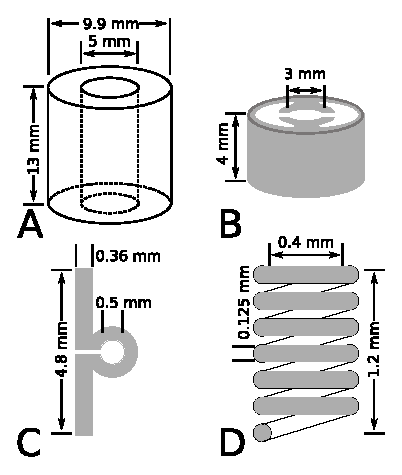
\includegraphics{Kapitel/Appendix/Images/S1-Geometries.eps}
 \caption[Geometries of resonators in this work.]{Dimensions and geometry of the four resonators compared in this paper. A) Bruker Biospin ER4118X-MD-5W1 (MD5W1) sapphire dielectric resonator, B) Bruker Biospin ER4118X-MS-3W1 (MS3) split-ring resonator, C) Planar Micro Resonator 0.5~mm inner loop diameter, and D) self-resonant micro-helix with a 0.4~mm inner diameter. Gray indicates metallic surfaces.}
 \label{fig:geo}
\end{figure}

The PMRs are fabricated by printing the micro-resonator geometry on a substrate using photo-lithographic techniques. \cite{Suter2005, Suter2008, suter2015} The planar micro-resonators show significant improvement in absolute spin sensitivity compared to the best commercial probe-heads available. \cite{ ReijerseSavitsky2017} PMRs can be produced relatively cheaply using semiconductor etching techniques and laser scribing, and configured for many frequencies with inner diameter sample sizes of 20-1000 $\mu$m. Furthermore, these structures offer excellent filling factors, high resonator efficiencies, and minimal power dissipation. It was recently demonstrated that a planar micro-resonators with Rogers RO6010LM substrate and a 500~$\mu$m sample diameter can be successfully employed for the study of crystals of inorganic metal complexes as well as [NiFe]-hydrogenase (0.35 $\times$ 0.2 $\times$ 0.2~mm$^3$) at 14~GHz, equipped with a specially designed cryogenic receiver at a temperature of 12~K. \cite{NARKOWICZ201379} Yet, such designs require a modified bridge to accommodate the cryogenic amplifier setup.

\begin{figure}[htbp]
\centering
 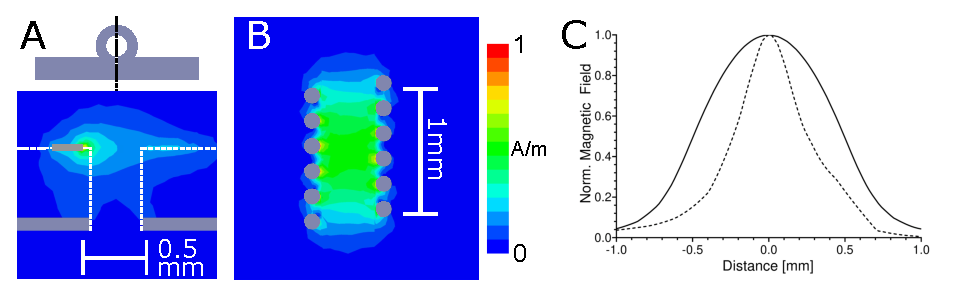
\includegraphics[width=\textwidth]{Kapitel/Ch4-Images/02-PMRCompare_OnAxis.eps}
 \caption[Ansys HFSS magnetic field simulation: PMR and micro-helix.]{Ansys HFSS finite-element modeling simulation of the microwave magnetic fields of a A) $\Omega$-shaped planar micro-resonator on sapphire substrate (dashed white lines; cut-plane shown on inset) with a 0.5~mm sample diameter over a ground plane and a B) 5.5 turn micro-helix with a 0.4~mm inner diameter. Normalized microwave magnetic field, for both resonators at the same power, is shown on the right. C) Normalized microwave magnetic field on axis of a $\Omega$-shaped planar micro-resonators on sapphire substrate with a 0.5~mm sample diameter over a ground plane (dashed lines) and a 6.5 turn micro-helix with a 0.4~mm inner diameter (solid).}
 \label{fig:HFSS}
\end{figure}

Due to their planar geometry, PMR designs are limited in their $Q$-value (50-180) and suffer from a strong inhomogeneity of the microwave magnetic field, illustrated in Fig.~\ref{fig:HFSS}A compared to the microwave magnetic field of the self-resonant micro-helix, Fig.~\ref{fig:HFSS}B. The microwave magnetic field comparison on axis can be found in Fig.~\ref{fig:HFSS}C. Improvement of the $Q$-value of the PMR geometry are reported here. By changing the substrate from Rogers RO6010LM substrate to single-crystal sapphire the $Q$-value increases by a factor of 3. The reduction of the $Q$-value using the Rogers RO6010LM substrate is partially due to surface roughness, and not just the loss tangent of the material. Because of these challenges, the PMRs have room for improvement and exploration of different geometries have led to the self-resonant micro-helix. Therefore, in this work, we compare the self-resonant micro-helix, general geometry shown in Fig.~\ref{fig:geo}D, to the planar micro-resonators.

Simulations, from the commercially available finite-element modeling program Ansys Electronics Desktop with HFSS (High Frequency Structure Simulator; v. 19.1), network analyzer, and experimental measurements of resonator characteristics are tabulated in Table~\ref{table:chars} and in Table~\ref{table:signal}. Simulations are performed assuming a fixed sample volume of 0.1~mm diameter by 0.1~mm height cylindrical sample. The simulated sample allows for absolute sensitivity comparisons amongst the resonator designs. Experimentally, a minuscule amount of lithium phthalocyanine (LiPC)\cite{Liu5438} is embedded in Crytoseal (or similar) wax and is used as a point sample. The LiPC sample produces a very sharp line width (less than 0.05~mT) in the presence of oxygen (narrower without oxygen present), saturates at large values of ${\mathbf B}_{1r}$, and one needs very little sample volume to observe the signal. Therefore the use of LiPC allows for a fair comparison between all resonators by using the same sample throughout the experiments. The term ``minuscule'' is defined as enough sample to observe a signal in the Bruker MD5W1 without causing line broadening in the micro-helix geometry. Such line broadening is due to a radiation dampening-like behavior caused by the very-large filling factor $\eta$.

Bench tests of resonator characteristics, such as the frequency measurements, $Q_0$-value, and sample frequency shifts, were performed on an Agilent 8722ES (now Keysight Technologies; Santa Rosa, CA, USA) vector network analyzer.

The photosystem II complex sample from spinach was prepared by following the BBY method and placed in a 0.4~mm outer diameter capillary with a 0.3~mm inner diameter. \cite{BBY1981} The tyrosine D (Y$_D^\bullet$) radical is generated by ambient light at room temperature for a few minutes and then rapidly frozen in liquid nitrogen. The Y$_D^\bullet$ radical is well-suited as a biological test sample since it has been extensively studied and the g- and hyperfine tensors are known. \cite{Hofbauer6623} Using UV-VIS spectroscopy, the number of chlorophyll molecules in the sample can be determined and, taking into account that there are approximately 250 chlorophyll molecules per photosystem II complex in spinach, the approximate amount of enzyme can be calculated. Each photosystem II complex contains one Y$_D^\bullet$ radical. For the sample prepared in this work, 7.9~$\mu$M/mL of chlorophyll molecules were measured, resulting in approximately 1.6$\times10^{12}$ Y$_D^\bullet$ radicals in the 85~nL that fill the micro-helix. 

Additionally, photosystem II core complex, extracted and purified from the thermophilic cyanobacterium {\em Thermosynechococcus elongatus}, has been crystallized to reach a crystal size of 0.3 $\times$ 0.18 $\times$ 0.18 mm$^3$, using the method of Athina Zouni and colleagues. \cite{KERN2005147} The crystals were gradually transferred to a cryogenic protection buffer (100~mM MES, pH 6.5, 5~mM CaCl$_2$ , 30\% (w/w) glycerol, 16\% PEG2000). The photosystem II core complex forms a dimer and the crystal has a unit cell space group symmetry P${2_1\,2_1\,2_1}$ which generates two asymmetric units per unit cell (PDB ID: 1W5C). From this one can calculate that there are approximately 8.9$\times10^{12}$ Y$_D^\bullet$ radicals in the test crystal. The active center and the Y$_D^\bullet$ of a cyanobacterium is equivalent to that of the photosystem II from spinach. 

\section{Theory and Design}
We focus on the development of resonant structures to increase EPR absolute spin sensitivity at X-band without the use of super-conducting materials, which require temperatures that are sub-optimal for metallo-enzyme research and exhibit $Q$-values too large for pulse experiment, or commercial bridge modifications, which require technical expertise not commonly available in EPR laboratories. We start with the well-established EPR signal analysis by Feher,\cite{FeherSignal} which states that the continuous-wave EPR signals for a critically-coupled resonator on a reflection bridge is proportional to
\begin{equation}
 S \propto \chi \eta Q P^{1/2},\label{eq:feher}
\end{equation}
where $\chi$ is the magnetic susceptibility, $Q$ is the $Q$-value of the cavity, $P$ is the incident power, and $\eta$ is the filling factor. The $Q$-value is defined as the ratio of the stored energy in the resonator to the power loss in the sample and resonator. \cite{ginzton1957microwave} While, the filling factor is defined as the ratio of the circularly polarized microwave magnetic field stored energy perpendicular to the static magnetic field that gives rise to EPR transitions and the complete magnetic field stored energy in the geometry,
\begin{equation}
 \eta = \frac{\int {\mathbf B}_{1r} \cdot {\mathbf B}_{1r}^* dV_s}{\int {\mathbf B}_1 \cdot {\mathbf B}_1^* dV},
\end{equation}
where ${\textbf B}_1$ is the microwave magnetic field in all space ($V$) and ${\textbf B}_{1r}$ is one component of the clockwise (or counter clockwise) rotational component of the linear ${\textbf B}_1$ field perpendicular to the static magnetic field in the sample volume ($V_s$). \cite{FeherSignal, misrabook}

From Eqn.~\ref{eq:feher}, we can derive a metric that encompasses the filling factor $\eta$ and the Q-value, called the resonator efficiency. \cite{hydehoff} The resonator efficiency (or, conversion factor) is defined as 
\begin{equation}
 \Lambda = \frac{\left|{\mathbf B}_{1r}\right|}{\sqrt{P_l}} \qquad [\text{mT/W}^{1/2}],
\end{equation}
where $P_l$ is the power loss in the system, including sample. However, $\Lambda$ assumes that the microwave magnetic field is uniform and does not take into account non-uniformity of the field over the sample. Experimentally, the microwave magnetic field is distributed throughout the sample and the average of $\Lambda$ is measured. We can define the resonator efficiency average as
\begin{equation}
 \Lambda_{ave} = \frac{\int |{\mathbf B}_{1r}| dV_s}{\sqrt{P_l} V_s} \qquad [\text{mT/W}^{1/2}].
\end{equation}
The resonator efficiency average is proportional to the signal and, for a fixed volume, is proportional to the absolute spin sensitivity. 

Cavity resonators, such as the Bruker Super High-Q probe head, are not sufficiently sensitive for extremely small samples since the very small filling factor $\eta$ is not compensated by the high Q-value, resulting in a poor EPR signal. \cite{ReijerseSavitsky2017} Therefore, one way to maximize $\Lambda_{ave}$ is to reduce the size of the resonant structure relative to the sample volume, increasing the filling factor. The challenge arises due to potentially increasing the losses in the system, degrading the Q-value, more than the increase in the filling factor. Two common methods to reduce the size of a resonant geometry is to either use dielectric resonators (DR) to reduce the wavelength and, consequently, the size of the resonator or loop-gap resonators (LGR) to reduce the cut-off frequency of a waveguide by introducing protrusions to create regions of inductive loops and capacitive gaps. (Dielectric resonator and LGR geometries with commercially available dimensions are illustrated Fig.~S1 and the microwave characteristics are tabulated in Table~\ref{table:chars}.) However, in order to study sample volumes less than 0.03~$\mu$L, further resonator reduction strategies are needed.

Limitations to minimizing LGR geometries stem from an increase in Ohmic losses due to a reduction in the gap spacing to maintain a constant resonant frequency as the sample-loop radius is reduced. In practice, this has put a limit on the $\Lambda_{ave}$ obtainable to less than 1~mT/W$^{1/2}$ for X-band. Further EPR signal improvement is possible using dielectric resonators by increasing the dielectric permittivity, and dielectric resonators with permittivity up to 80 have been used for continuous-wave EPR experiments on crystals of porous materials and polymers. \cite{dielectricReson1, dielectricReson2} However, such resonators exhibit Q-values over 2500 that make pulse experiments problematic. \cite{Friedlaender2015} 

Several other approaches have been followed to develop application-specific resonators for micro-samples: microstrip resonators (MR)\cite{Microstrip2009, GhirriMicroStrip}, ultra-miniature micro-resonators (UMR, 2-150 $\mu$m)\cite{AharonBlankUltra2013}, surface loop-gap micro-resonators (LGMR, 50-150 $\mu$m)\cite{AharonSurface2010}, very high-permittivity dielectric resonators \cite{walsh86, GOLOVINA200852}, and planar micro-resonators. \cite{Suter2005, Suter2008, suter2015} All of which significantly reduce the size of the resonator, but have challenges that limit the usefulness for single-crystal experiments. Herein, we introduce a new type of resonator based on a self-resonant micro-helix which is particularly useful for protein single-crystal experiments at X-band and can be used as a drop-in replacement on a standard commercial system. The self-resonant micro-helix geometry, illustrated in Fig.~\ref{fig:fabricated}, solves these challenges by providing good magnetic field homogeneity, a high efficiency parameter, an optimum $Q$-value for both pulse and continuous-wave EPR experiments, straight-forward impedance matching, and ease of sample placement. 

Helical resonators were first introduced to EPR in the early-1960s as a method to increase the microwave magnetic field at the sample. Resonant helical geometries were affixed to one end of a shorted waveguide creating a slow-wave structure. \cite{Webb1962, Helix1967} Coupling was achieved by direct connection to a coaxial line with a capacitive matching network or by microwave incident on the helical structure from a waveguide. The sample was placed within the helix and showed reasonable sensitivity increase and larger microwave magnetic field due to higher filling factors compared to typical cavities. \cite{Nolle1966} Broadband slow-wave helical resonators were employed for multi-frequency experiments, where a non-resonant structure, having a $Q$-value close to unity, could be matched with a slide-screw tuner over an octave bandwidth. \cite{nonresonant1986} However, over time, they were replaced by loop-gap resonators which achieved higher concentration sensitivity for limited samples.\cite{froncisz1982loop}

Recently, micro-coils have gained popularity in NMR for nano-liter samples \cite{Olson1967, SUBRAMANIAN1998227, cr980140f,Kentgens2008,Raluca2011,Jones2012} and for microfluidics. \cite{Mompean2018} However, three characteristics differentiate our micro-helix configuration from those described in the EPR \cite{Webb1962, Helix1967, oldmicro} and NMR literature\cite{WEBB2005892}: i) the helix is self-resonant, meaning that the self-inductance of $n$-turns ($L_{tot}$) and self-capacitance between the loops ($C_{tot}$) resonate at a frequency determined by $\omega^2 L_{tot}C_{tot}=1$, where $\omega$ is the resonant frequency in radians/s. Since the geometry is self-resonant, no additional capacitors are needed. A self-resonant micro-helix has lower Ohmic loss, which provides a higher $Q$-value than is typically feasible with micro-coil geometries in NMR, where, with an NMR micro-coil, a typical $Q$-value is around 30. \cite{WEBB2005892} With a self-resonant micro-helix, the volume to surface ratio is maximized and a $Q$-value of 300 is achievable. ii) The helix length is much smaller than the wavelength (31.6~mm at 9.5~GHz), which increases the uniformity and the inner diameter is 0.4~mm at X-band, which increases the resonator efficiency. With this geometry, the micro-helix is not a slow-wave structure but an inductor at self-resonance. The microwave magnetic field profile is shown in Fig.~\ref{fig:fabricated}D. iii) Finally, the helix is coupled to an inductive coupling loop on a printed-circuit board by mutual inductance, which can be designed to minimize noise and further increase the EPR signal-to-noise ratio. \cite{coupling2016} Additionally, mutual inductance coupling does not require a balun or capacitive matching networks, simplifying coupling methods.

\paragraph{Qualitative Sensitivity Comparison of the X-band micro-helix to High-frequency single-mode resonators.}
Simulations were performed in commercial finite-element modeling software, Ansys Electronics Desktop with HFSS (High Frequency Structure Simulator; v. 19.1), comparing a cylindrical TE$_{011}$ cavity at W-band to the micro-helix geometry using a 85~nL frozen solution sample. Assuming no g-anisotropy, the W-band TE$_{011}$ exhibits a factor of approximately 3 in improved EPR signal intensity compared to the micro-helix geometry at X-band. However, for example, the g-anisotropy at W-band spreads the tyrosine D radical in photosystem II spectrum by a factor of 2 (see Fig.~2 in Ref.~[5.\kern-0.4em\citenum{Hofbauer6623}]); for some systems, the g-anisotropy may be more severe. Therefore, the micro-helix EPR sensitivity at X-band is comparable to a standard W-band system with a cylindrical TE$_{011}$ cavity. 

As the frequency becomes even higher, the resonator efficiency decreases due to losses on the surface of the resonator. For example, the Bruker 263~GHz single-mode resonator has a reported $\Lambda_{ave}$-value of 0.7 mT/W$^{1/2}$. \cite{bruker263} This is approximately half of the cylindrical TE$_{011}$ cavity at W-band. The lower $\Lambda_{ave}$ leads to only a factor of five in EPR signal improvement compared to the micro-helix at X-band. However, g-anisotropy becomes more severe as the operating frequency increases.

Therefore, the micro-helix geometry opens up the possibility to perform multi\-/frequency EPR on the same sample from X-band to 263~GHz. Using a 0.4~mm outer diameter capillary, a sample can be placed in the micro-helix at X-band and the same sample can then be inserted into a W-band (94~GHz) or 263~GHz cavity. This ability allows for complimentary techniques to be used for disentangling the angle dependencies of hyperfine-tensor interactions.

\section{Results and Discussion}
\subsection{EPR Characteristics Comparison of Resonators.}
Good agreement is shown in Table~\ref{table:chars} and in Table~\ref{table:signal}. The lower measured $Q$-value of the self-resonant micro-helix is due to losses associated with the Polytetrafluoroethylene (PTFE) substrate of the printed-circuit board and losses in the super-glue adhesive. Further work to minimize these losses is underway.

\begin{table}[htbp]
\centering
\caption[Resonator characteristics calculated and measured.]{Resonator characteristics calculated and measured. Calculations use fixed volume sample of dimension  0.1~mm diameter by 0.1~mm height cylindrical sample while measurements use a minuscule amount of lithium phthalocyanine (LiPC) in a 0.4~mm outer diameter and 0.3~mm inner diameter capillary tube. The P$_{1/2}$-values are measured from the power saturation curve and are related to the calculated $\Lambda_{ave}^2$. The $\Lambda_{ave}$ measurements were made by a 2\% w/w BDPA ($\alpha$,$\gamma$-Bisdiphenylene-$\beta$-phenylallyl; Sigma-Aldrich Chemicals; CAS number 35585-94-5) in polystyrene with dimensions of 0.55$\times$0.18$\times$0.08~mm$^3$.}
\label{table:chars}
\begin{tabular}{l|c|c|c|c|c}
\multicolumn{1}{l}{} & DR & LGR & \multicolumn{2}{c|}{PMR} &  \\
\multicolumn{1}{c||}{Geometry} & MD5W1 & MS3 & 6010LM & Sapphire & Micro-Helix \\ \hline \hline
\multicolumn{1}{l||}{Freq. Calc.} & \multicolumn{1}{c|}{9.67} & \multicolumn{1}{c|}{9.67} & \multicolumn{1}{c|}{9.87} & \multicolumn{1}{c|}{9.87} & 9.78 \\ \hline 
\multicolumn{1}{l||}{Freq. Meas.} & \multicolumn{1}{c|}{9.69} & \multicolumn{1}{c|}{9.69} & \multicolumn{1}{c|}{9.58} & \multicolumn{1}{c|}{9.58} & 9.73 \\ \hline 
\multicolumn{1}{l||}{$Q_0$-value Calc.} & \multicolumn{1}{c|}{8860} & \multicolumn{1}{c|}{870} & \multicolumn{1}{c|}{90} & \multicolumn{1}{c|}{190} & 360 \\ \hline 
\multicolumn{1}{l||}{$Q_0$-value Meas.} & \multicolumn{1}{c|}{6650} & \multicolumn{1}{c|}{600} & \multicolumn{1}{c|}{61} & \multicolumn{1}{c|}{181} & 220 \\ \hline
\multicolumn{1}{l||}{$\Lambda$ Calc. {[}mT/W$^{1/2}${]}} & \multicolumn{1}{c|}{0.60} & \multicolumn{1}{c|}{0.68} & \multicolumn{1}{c|}{1.9} & \multicolumn{1}{c|}{2.9} & 4.1 \\ \hline 
\multicolumn{1}{l||}{$\Lambda_{ave}$ Calc. {[}mT/W$^{1/2}${]}} & \multicolumn{1}{c|}{0.60} & \multicolumn{1}{c|}{0.68} & \multicolumn{1}{c|}{1.5} & \multicolumn{1}{c|}{2.6} & 4.0 \\ \hline 
\multicolumn{1}{l||}{P$_{1/2}$ Meas. {[}mW{]}} & \multicolumn{1}{c|}{19.2} & \multicolumn{1}{c|}{18.4} & \multicolumn{1}{c|}{17.3} & \multicolumn{1}{c|}{1.8} & 0.8 \\ \hline 
\multicolumn{1}{l||}{$\Lambda_{ave}$ Meas. {[}mT/W$^{1/2}${]}} & \multicolumn{1}{c|}{–} & \multicolumn{1}{c|}{–} & \multicolumn{1}{c|}{–} & \multicolumn{1}{c|}{2.2} & 3.2
\end{tabular}
\end{table}


\paragraph*{Comparison of a Planar micro-Resonator and micro-Helix}
In Chapter 5, the planar micro-resonator (PMR) \cite{Suter2005,Suter2008,suter2015} and micro-Helix geometries are thoroughly introduced. In this section we will construct an eigenmode solution of both the PMR and micro-helix to compare how the signal and resonator efficiency $\Lambda_{ave}$ scale with a lossy aqueous sample ($\epsilon_r = 63 - i26.46$ from Ref.~[2.\kern-0.4em\citenum{EllisonWater2017}]) and relatively-lossless ice sample ($\epsilon_r=3.17-i0.0035$ from Ref.~[2.\kern-0.4em\citenum{icedielectric}]). 

The files can be found at https://github.com/jsidabras/HFSSTutorial and the Ansys \textit{aedt} file has 4 projects to be solved. The projects created use local variables for performing parametric sweeps. For instance, the sample radius on both geometries can be varied and this parameter will be used in this comparison. Mesh operations have been added on the quartz capillary tube and on the surface of the main resonator geometry to reduce numerical fluctuations and obtain a field profile void of discontinuities. An eigenmode solution is used for simplicity. 

\begin{figure}[ht]
 \centering
 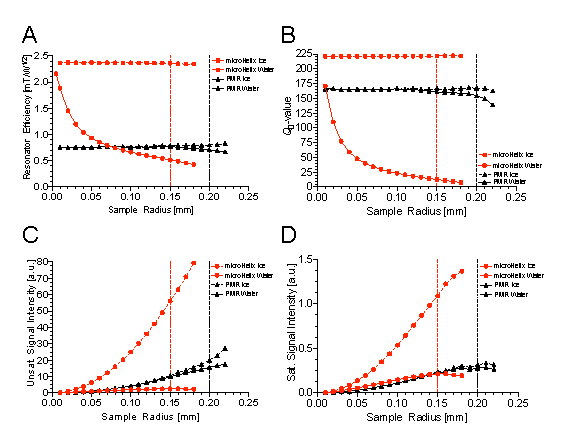
\includegraphics[width=\textwidth]{Kapitel/Ch2-Images/Ch2-SweepOutput.eps}
 \caption[EPR characteristics as the sample radius is swept.]{EPR characteristics for the PMR with sapphire substrate (black; $\blacktriangle$) and the 0.4~mm micro-helix (red; $\CIRCLE$) with a water (solid) and ice (dashed) sample. Shown are the EPR characteristics as the sample radius is swept for the A) resonator efficiency $\Lambda$, B) $Q_0$-value, C) unsaturated EPR signal, and D) saturable EPR signal. The dashed-dot lines indicate the largest practical capillary inner radius for the helix (red) and PMR (black).}
 \label{fig:SweptData}
\end{figure}

Shown in Fig.~\ref{fig:SweptData} are the simulated EPR characteristics for the micro-helix (red; $\CIRCLE$) and planar micro-resonator (black; $\blacktriangle$) geometries. The ice sample is shown as a dashed line, while the aqueous sample is shown as a solid line. The sample radius is swept and a quartz sample holder with a wall thickness of 0.025~mm is used. The dashed-dot line indicates the largest commercially available practical capillary inner radius for the helix (red) and PMR (black). In this study, we focus on a ``concentration sensitivity'' comparison. By comparing ``concentration sensitivity'' we focus on the resonator performance assuming a varying sample volume at a fixed concentration.

\begin{figure}[ht]
 \centering
 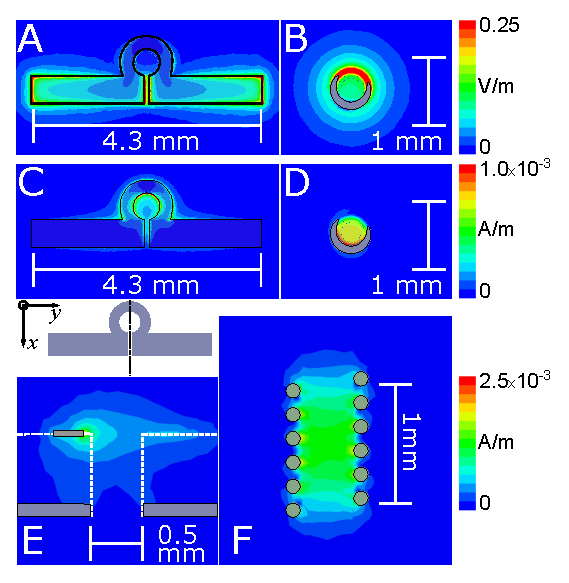
\includegraphics[width=0.9\textwidth]{Kapitel/Ch2-Images/Ch2-AnsysFields.eps}
 \caption[Simulated field distribution for Helix and PMR.]{Simulated field distribution for the magnitude of the electric field for the A) planar micro-resonator and B) micro-helix and the magnitude of $\mathbf{H_{1r}}$ with $\mathbf{H}_0$ in the $y$-direction for the C) planar micro-resonator and D) micro-helix in the $x$-$y$-plane. And the magnitude of $\mathbf{H_{1r}}$ with $\mathbf{H}_0$ in the $y$-direction for the E) planar micro-resonator and F) micro-helix in the $x$-$z$-plane. }
 \label{ch2-fig:FieldData}
\end{figure}

For the PMR (black; $\blacktriangle$), little change in both the average resonator efficiency $\Lambda_{ave}$ and $Q_0$-value is exhibited as the sample radius is increased, Figs.~\ref{fig:SweptData}A and \ref{fig:SweptData}B, respectively. From the simulations we can see that the electric field, which gives rise to losses, is well contained in the planar micro-resonator geometry away from the sample loop. Shown in Fig.~\ref{ch2-fig:FieldData}A is a plot of the magnitude of the electric field. A potential is formed across the PMR gap and a gradient of charge is formed in the loop which goes to zero opposite of the gap. This is similar to the electric field profile of a one-loop--one-gap loop-gap resonator.  

In the PMR, the value of $\Lambda_{ave}$ is approximately one third of the micro-Helix (red $\CIRCLE$; in Fig.~\ref{fig:SweptData}A). The reduction in $\Lambda_{ave}$ is due to a significant portion of the magnetic field stored energy being located outside of the sample volume in the PMR geometry and significant inhomogeneity of the magnetic field along the axis. This is illustrated in Fig.~\ref{ch2-fig:FieldData}C where the magnitude of $\mathbf{H_{1r}}$ with $\mathbf{H}_0$ in the $x$-direction is plotted. The quantity $\mathbf{H_{1r}}$ is the magnetic field that gives rise to the EPR signal and a significant portion of this magnetic field lies outside of the sample region. This is also true along the axis, shown in Fig.~\ref{ch2-fig:FieldData}E, where a large gradient of $\mathbf{H_{1r}}$ is present. 

With the micro-helix geometry, the $\mathbf{H_{1r}}$ is concentrated in the center and very little magnetic field is found outside of the sample volume, shown in Fig.~\ref{ch2-fig:FieldData}D. Additionally, the $\mathbf{H_{1r}}$ field profile along the axis is more homogeneous compared to the PMR, shown in  Fig.~\ref{ch2-fig:FieldData}F. The homogeneous magnetic field in the micro-helix leads to a higher filling factor $\eta$ and, ultimately, a higher average resonator efficiency $\Lambda_{ave}$, as shown in Fig.~\ref{fig:SweptData}A.

As anticipated from Eqn.~\ref{ch2-eq:su}, relatively lossless samples will display EPR unsaturable signal growth that is proportional to the magnetic field squared within the sample volume, shown in Fig.~\ref{fig:SweptData}C as a dashed line for the micro-helix (red; $\CIRCLE$) and PMR (black; $\blacktriangle$). With such samples, the EPR signal expected by using the micro-helix is significantly enhanced compared to the PMR. In contrast, the saturable sample defined by  Eqn.~\ref{ch2-eq:ss} has a maximum due to the interplay of the power loss $P_l$ and the magnetic field in the sample. Since the micro-helix exhibits an azimuthal component of the electric field that penetrates into the sample, shown in Fig~\ref{ch2-fig:FieldData}B, lossy aqueous samples are problematic in this geometry. Likewise, the  resonator efficiency $\Lambda_{ave}$ and $Q_0$-value are significantly reduced as the diameter of the aqueous sample increases, shown in Fig.~\ref{fig:SweptData}A and \ref{fig:SweptData}A, respectively.

Aqueous sample simulations show that the PMR losses do not increase with the size of the sample and little changes of the unsaturable and saturable signal are illustrated, shown as a solid black line in Figs.~\ref{fig:SweptData}C and \ref{fig:SweptData}D. Compared to the micro-helix geometry with lossy aqueous samples, the PMR performs 5 times better for experiments at the same microwave power (unsaturable signal) and 50\% better for the experiments at same microwave field (saturable signal). This means the PMR geometry may be advantageous for room temperature samples and further improvement to the PMR to increase the filling factor $\eta$ is underway. 

\begin{figure}[ht]
 \centering
 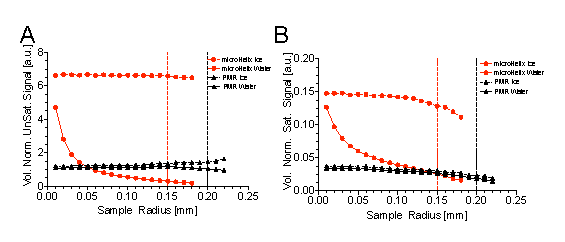
\includegraphics[width=\textwidth]{Kapitel/Ch2-Images/Ch2-AbsSweepOutput.eps}
 \caption[Volume normalized swept EPR signal optimization.]{Volume normalized Swept EPR signal for the PMR with sapphire substrate (black; $\blacktriangle$) and the 0.4~mm micro-helix (red; $\CIRCLE$) with a water (solid) and ice (dashed) sample. Shown are the data fro the A) unsaturated EPR signal and B) saturable EPR signal normalized to sample volume. The active region of the micro-helix and planar micro-resonator is assumed to be 1.2~mm and 1.1~mm, respectively. The dashed-dot line indicates the largest practical capillary inner radius for the helix (red) and PMR (black).}
 \label{fig:AbsSweptData}
\end{figure}

This example assumed the sample tube is completely filled and extends beyond the active region. It is noted that, the active length of the two resonators is different and the data plotted in Fig.~\ref{fig:SweptData} can be normalized to the active volume and a comparison of the ``absolute sensitivity'' can be performed. Based on the magnetic field profile of  Figs.~\ref{ch2-fig:FieldData}E and \ref{ch2-fig:FieldData}F, the active region of the micro-helix and planar micro-resonator is assumed to be 1.2~mm and 1.1~mm, respectively, and a volume normalized signal is plotted in Fig.~\ref{fig:AbsSweptData}. Comparing the resonators at a equivalent sample volume is the focus of Chapter~5 for single-crystal EPR of with sample volumes smaller than 27~nL. At a fixed sample volume, the losses in the micro-helix associated with the aqueous sample still significantly affect the performance of the resonator, plotted in Figs.~\ref{fig:AbsSweptData}A and \ref{fig:AbsSweptData}B as a solid line for the micro-helix (red; $\CIRCLE$). However, compared to the PMR (black; $\blacktriangle$) there exists some sample volumes where the micro-helix yields a higher EPR signal. Finally, at a fixed sample volume and a relatively lossless sample, the micro-helix significantly outperforms the PMR geometry, plotted in Figs.~\ref{fig:AbsSweptData}A and \ref{fig:AbsSweptData}B as a dashed lines.

This simple optimization sweep teaches about differences in such simple geometries and leads to intuition for further performance improvements. For instance, there is room for improvement for small volume aqueous samples. Such improvements would focus on reducing the electric field in the sample while maintaining good magnetic field homogeneity. 


\paragraph{Power Saturation and $\Lambda_{ave}$ Measurements}
Power saturation experiments were performed using the LiPC sample and plotted in Fig.~\ref{fig:lipcpwrsat}. From the power saturation data, an unsaturable signal, saturable signal, and P$_{1/2}$-value measurement can be ascertained. The unsaturable signal is measured at constant microwave power (0.01~mW), while the saturable signal is measured at the power where the EPR signal amplitude is maximum (P$_{1/2}$-value; indicated by $\Diamond$). At the P$_{1/2}$-value, the B$_{1r}$ over the sample is identical in each of the resonators. For the power saturation experiments used in this work the microwave power was stepped in 3~dB increments from 200~mW to 0.2~$\mu$W (0-60~dB). Each scan was 30~s over 1~mT with 4096 pts, receiver gain of 60~dB and 100~kHz field modulation at 0.1~mT in all resonators. The over-modulation of the LiPC sample was used to increase the sensitivity in the Bruker commercial resonators while increasing the intrinsic line width (line-height--line-width compromise, discussed in Ref.~[5.\kern-0.4em\citenum{eaton2010quantitative}]). 

\begin{figure}[htbp]
\centering
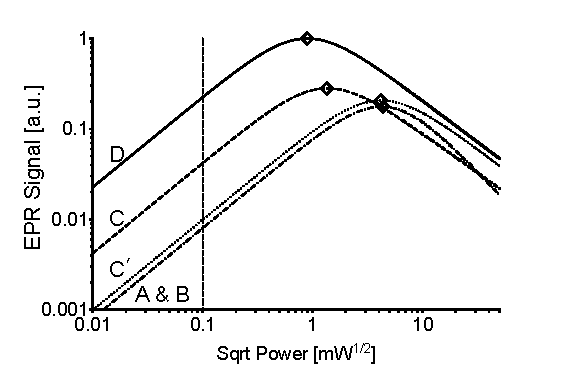
\includegraphics{Kapitel/Appendix/Images/S4-LiPCPowerSat.eps}
\caption[Power saturation data of LiPC comparing resonators.]{Power saturation data of LiPC showing the A) Bruker MD5 (dash-dot), and B) Bruker MS3, $\Omega$-type PMR with 0.5~mm sample loop with C) sapphire substrate (dashed) and C$'$) Rogers 6010LM substrate (dotted), and D) micro-helix (solid). EPR saturable signal is taken at peak signal (P$_{1/2}$-value, constant microwave field; indicated by $\Diamond$), while EPR unsaturable signal is taken at 0.01~mW (constant microwave power; dotted line).}
\label{fig:lipcpwrsat}
\end{figure}

The ratio of two P$_{1/2}$-values can be compared to the square of the ratio of $\Lambda_{ave}$. The data for the Bruker MS3 and MD5W1, in our hands, lay on top of each other for the LiPC point sample. Simulated and measured EPR signal amplitude characteristics are tabulated in Table~\ref{table:chars} and in Table~\ref{table:signal}. 

In order to measure the $B_{1r}$ directly, a series of pulse nutation experiments were performed. \cite{schweiger2001principles} The pulse nutation experiments were performed with an echo detected EPR signal using a 40~ns $\pi$/2 pulse and a pulse separation of 300~ns. A HA6047 300~W amplifier (HBH Microwave GmbH, Stutensee, DE) was used for all resonators and the power attenuation was adjusted for maximum echo. From the nutation experiment oscillations one can use the equation,
\begin{equation}
 B_{1r} = \frac{2 \pi}{t \gamma} \qquad \text{[G]},
\end{equation}
where $\gamma$ is the gyromagnetic ratio of a free electron and $t$ is the time in seconds for a whole ($2\pi$) oscillation, to calculate the  $B_{1r}$ in Gauss. Then value of $B_{1r}$, is converted to mT (divide by 10) and normalized to the incident power by,
\begin{equation}
\Lambda_{ave} = \frac{B_{1r}}{(P/2^{\zeta/3})^{1/2}}\qquad [\text{mT/W}^{1/2}],
\end{equation}
where $P$ is the maximum power available (in this case, 300~W) and $\zeta$ is the attenuation of that power set on the console in dB. 

The sample was a 2\% w/w BDPA ($\alpha$,$\gamma$-Bisdiphenylene-$\beta$-phenylallyl; Sigma-Aldrich Chemicals; CAS number 35585-94-5) in polystyrene and, in our laboratory, is used as a pulse EPR standard. The PS and BDPA are fully dissolved in toluene, laid out onto a covered Pyrex Petri dish, and left to evaporate for several days. The sample is then cut and placed in the sample tube for further testing. For a direct measurement of $\Lambda_{ave}$, an EPR nutation experiment was performed at three pulse powers using the 2\% w/w BDPA in polystyrene and cut to 0.55 $\times$ 0.18 $\times$ 0.08~mm$^3$. The micro-helix has measured power conversion efficiency parameter of 3.2~mT/W$^{1/2}$ which corresponds, for an S=1/2 spin system with g=2, to a $\pi/2$ pulse of 20~ns with an incident power of approximately 20~mW. No signal was measurable in the PMR RO6010LM, MS3, and MD5W1 due to lack of sensitivity. However, the PMR with a sapphire substrate has a good efficiency parameter of 2.2~~mT/W$^{1/2}$ which corresponds, for an S=1/2 spin system with g=2, to a $\pi/2$ pulse of 20~ns with an incident power of approximately 40~mW. These data are tabulated in Table~\ref{table:chars}.

\paragraph{Performance compared to commercially available and state-of-the-art microwave probes.}
The self-resonant micro-helix geometry wound around a 0.4~mm capillary is shown in Fig.~\ref{fig:fabricated}A. The final number of the micro-helix windings is determined by the pitch of the helix, the quartz capillary sample tube (0.4~mm outer diameter 0.3~mm inner diameter), and the surrounding Rexolite which all affect the resonance frequency. The 6.5-turn micro-helix had a resonant frequency around 9.7~GHz when coupled to the printed-circuit board inductive coupler. The micro-helix assembly is attached to a custom insert that is compatible with commercial EPR systems. The complete structure is shown in Fig.~\ref{fig:fabricated}B with an expanded view of the printed-circuit board geometry in Fig.~\ref{fig:fabricated}C. Comparison of the fabricated micro-helix geometry with commercial (Bruker MD5W1 and Bruker MS3) and state-of-the-art (PMR; based on Rogers RO6010LM printed-circuit board or sapphire substrates) microwave probes is provided in Table~\ref{table:signal}. The micro-helix exhibits the highest absolute sensitivity with no modification to the commercial bridge. 

As described in Table~\ref{table:signal}, if the EPR signal cannot be saturated (UnSat.) a factor of approximately 28 can be achieved compared to commercially available probeheads. EPR signals that cannot be saturated are proportional to the square root of the incident microwave power and, therefore, the EPR signal intensity is only limited by the amount of power available. However, most protein samples saturate readily, and, as such, the maximum signal that can be obtained is determined by the microwave magnetic field at the sample. When the sample is saturable (Sat.), a factor of 5.7 can be achieved. 

\begin{table}[htbp]
\centering
\caption[Resonator EPR signal characteristics calculated and measured.]{Resonator EPR signal characteristics calculated and measured for a fixed sample volume.}
\label{table:signal}
\begin{tabular}{l|l|l|l|l}
 & \multicolumn{2}{l|}{UnSat. Signal} & \multicolumn{2}{l}{Sat. Signal}\\
Geometry & Calc. & Meas. & Calc. & Meas.\\ \hline \hline
Bruker MD5W1 & 1.0 & 1.0 & 1.0 & 1.0 \\ \hline
Bruker MS3 & 1.5 & 1.2 & 1.0 & 1.0 \\ \hline
PMR RO6010LM & 4.4 & 1.2 & 0.9 & 1.2 \\ \hline
PMR Sapphire & 18.6 & 13.3 & 3.9 & 3.8 \\ \hline
Micro-Helix & 35.7 & 28.2 & 6.1 & 5.7 \\
\end{tabular}
\end{table}

\subsection{EPR of Photosystem II tyrosine D radical}
We seek to test the micro-helix geometry with a protein sample, specifically, photosystem II. In photosystem II, water oxidation takes place at the tetranuclear manganese cluster, with a redox-active tyrosine radical (Y$_Z^\bullet$) as an interface to the light-induced electron transfer process. \cite{STYRING201276} Symmetrically to Y$_Z^\bullet$, a long-lived tyrosine radical (Y$_D^\bullet$) exists in the second branch of the photosystem II which contains no manganese cluster. In this work, the Y$_D^\bullet$ radical is used as a standard probe because it is stable for a number of hours under ambient conditions\cite{Saito7690} and has been well-characterized using a variety of EPR techniques. \cite{Hofbauer6623, STYRING201276} The hyperfine interactions from several protons, both on the phenyl ring and distal CH$_2$ carbon, lead to the distinct splittings of the radical (S=1/2). To generate the tyrosine radical (Y$_D^\bullet$) EPR signal, the photosystem II core complex samples are illuminated in ambient light and rapidly frozen. 

The tyrosine D radical (Y$_D^\bullet$) of photosystem II is measured in two forms: (i) a frozen solution sample of photosystem II (BBY particles) \cite{BBY1981} placed in a 0.3~mm inner diameter capillary and (ii) a 0.3 $\times$ 0.18 $\times$ 0.18~mm$^3$ single crystal of photosystem II core complexes. \cite{KERN2005147} In both photosystem II samples, the Y$_D^\bullet$ and first ligand-sphere are known to be identical. These samples provide a benchmark for future work.

\paragraph{Frozen solution EPR of Photosystem II tyrosine D radical (Y$_D^\bullet$).}
\begin{figure}[htbp]
\centering
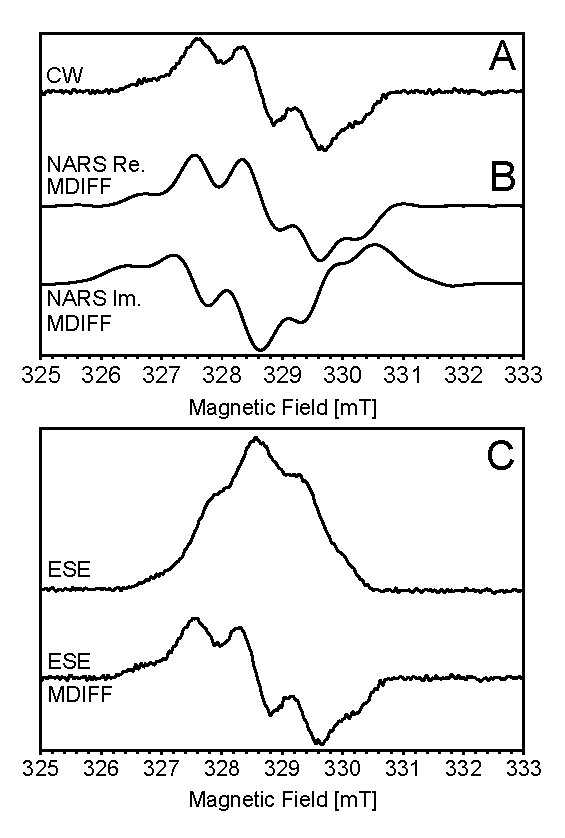
\includegraphics{Kapitel/Ch4-Images/02-PSII-BBY-Data.eps}
\caption[Frozen solution EPR on a 85~nL volume sample at X-band.]{Frozen solution EPR on a 85~nL volume sample at X-band Three EPR experiments performed with a 0.4~mm inner diameter self-resonant micro-helix. Shown are the A) continuous-wave, B) real and imaginary non-adiabatic rapid scan (NARS), and C) field-swept two-pulse electron spin-echo (ESE) EPR experiments of the tyrosine D radical (Y$_D^\bullet$) in photosystem II with 85~nL of frozen solution sample at a temperature of 80~K. Calculated moving difference (MDIFF) pseudo-modulation of 0.5~mT is shown for the NARS and field-swept ESE experiments in order to directly compare to the continuous-wave EPR experiment. The total time for the experiments were 49, 55, and 45 minutes, respectively. The signal-to-noise ratio is calculated and tabulated in Table~\ref{table:snrcalc}.}
\label{fig:BBYPSII}
\end{figure}

Shown in Fig.~\ref{fig:BBYPSII} is the Y$_D^\bullet$ radical EPR signal in an 85~nL frozen solution from photosystem II (BBY particles) at a temperature of 80~K using the self-resonant micro-helix. A continuous-wave EPR experiment, shown in Fig.~\ref{fig:BBYPSII}A, was performed an Elexsys E580 X-band bridge by sweeping 10~mT in 1 minute (4096 points) with a modulation rate of 100~kHz and an amplitude of 0.5~mT. The data was averaged 49 times for a total of 49 minutes at an incident power of 0.2~$\mu$W. To further improve the signal-to-noise ratio of the continuous-wave experiment, a field-swept non-adiabatic rapid scan (NARS) experiment was performed, data shown in Fig.~\ref{fig:BBYPSII}B. The field-swept non-adiabatic rapid scan (NARS) experiment was performed on the same commercial hardware using the rapid-scan method of M\"{o}ser {\em et al.}\cite{MOSER2017} and processed with the method described in Hyde {\em et al.}\cite{Hyde2013MDIFF} Herein, the scan rate was a sinusoidal 100~kHz field-sweep at 1~mT amplitude and a field-step size of 0.05~mT. The collected real and imaginary, pure-absorption and pure-dispersion, spectra were pseudo-modulated with a 0.5~mT moving difference (MDIFF)\cite{Hyde2013MDIFF} to compare to the field-modulated continuous-wave experiment. A factor of 2 in signal-to-noise improvement is obtained for the same signal acquisition time. 

A field-swept two-pulse electron spin-echo (ESE) EPR experiment was performed on the same commercial hardware over a 8~mT sweep, shown in Fig.~\ref{fig:BBYPSII}C. The field-swept ESE data was pseudo-modulated with a 0.5~mT MDIFF to compare the experiment with the field-modulated continuous-wave experiment of Fig.~\ref{fig:BBYPSII}A. The signal-to-noise ratio for all three experiments were calculated and tabulated in Table~\ref{table:snrcalc}. 

\begin{table}[htbp]
\centering
\caption[Signal-to-noise calculations.]{Signal-to-noise calculations for the three experiments performed on the photosystem II Y$_D^\bullet$ radical in frozen solution at a temperature of 80~K. Approximately 1.6$\times10^{12}$ spins were calculated to be in the 85~nL that fill the micro-helix.}
\begin{tabular}{llll}
\multicolumn{1}{l|}{Experiment} & \multicolumn{1}{l|}{SNR Re.} & \multicolumn{1}{l|}{SNR Im.} & Time\\ \hline\hline
\multicolumn{1}{l|}{Continuous Wave} & \multicolumn{1}{c|}{197} & \multicolumn{1}{c|}{131} & \multicolumn{1}{c}{49~min} \\\hline
\multicolumn{1}{l|}{NARS} & \multicolumn{1}{c|}{4400} & \multicolumn{1}{c|}{2300} & \multicolumn{1}{c}{55~min} \\\hline
\multicolumn{1}{l|}{NARS (MDIFF)} & \multicolumn{1}{c|}{410} & \multicolumn{1}{c|}{423} & \multicolumn{1}{c}{--} \\\hline
\multicolumn{1}{l|}{ESE} & \multicolumn{1}{c|}{248} & \multicolumn{1}{c|}{--} & \multicolumn{1}{c}{45~min} \\\hline
\multicolumn{1}{l|}{ESE (MDIFF)} & \multicolumn{1}{c|}{106} & \multicolumn{1}{c|}{--} & \multicolumn{1}{c}{--}\\
\end{tabular}\label{table:snrcalc}
\end{table}

\begin{figure}[htbp]
\centering
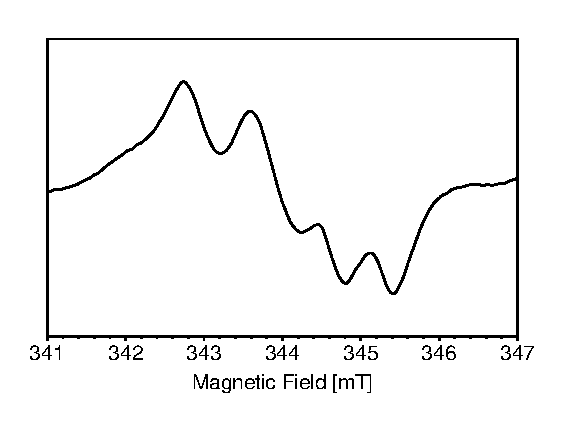
\includegraphics{Kapitel/Appendix/Images/S5-BBYMD5.eps}
\caption[CW EPR of frozen solution photosystem II in the Bruker MD5W1.]{Continuous-wave EPR of frozen solution photosystem II sample performed in the Bruker MD5W1 dielectric resonator at a temperature of 80~K. A signal-to-noise ratio of approximately 300 is calculated for 636~nL of sample.}
\label{fig:BBYMD5}
\end{figure}

Finally, a comparison between the MD5W1 dielectric resonator and the self-resonant micro-helix was performed with the frozen solution photosystem II (BBY particle) sample at a temperature of 80~K. A continuous-wave EPR experiment was performed to compare the EPR signal obtained with 85~nL volume in the micro-helix. The photosystem II sample was placed in a 0.3~mm inner diameter quartz tube with a sample height of 9~mm (636~nL) and centered in the dielectric cavity. A signal-to-noise ratio of approximately 300 is calculated for the 636~nL of sample, shown in Fig.~\ref{fig:BBYMD5}. The spectrum was collected by sweeping 10~mT in 1 minute (4096 points) with a modulation rate of 100~kHz and an amplitude of 0.5~mT. The data are averaged 49 times for a total time of 49 minutes at an incident power of 3.1~$\mu$W. This power was chosen to compare the two samples at approximately the same microwave magnetic field incident on the sample. Normalizing the signal-to-noise ratio with the volume yields a factor of approximately 5 improvement of absolute spin sensitivity using the self-resonant micro-helix compared to the MD5W1. These experiments serve to show the versatility of the micro-helix to perform EPR experiments on limited sample volumes (less than 85~nL) at X-band.

\paragraph{Single-Crystal continuous-wave EPR of the tyrosine D radical (Y$_D^\bullet$) in photosystem II core complex.}
Shown in Fig.~\ref{fig:xTalPSII} is continuous-wave EPR data collected at two separate angles of the photosystem II Y$_D^\bullet$ radical in a single crystal at a temperature of 80~K as a sensitivity test for the 0.4~mm inner diameter self-resonant micro-helix. The photosystem II core complex crystal had a volume of 0.3 $\times$ 0.18 $\times$ 0.18~mm$^3$. The spectra were collected by sweeping 15~mT in 1 minute (4096 points) with a modulation rate of 100~kHz and an amplitude of 0.3~mT. The data are averaged 49 times for a total time of 49 minutes at an incident power of 0.2~$\mu$W. Simulations using the known $g$-tensor and hyperfine tensors \cite{Hofbauer6623} were performed with an Easyspin (http://easyspin.org, Ref.~[5.\kern-0.4em\citenum{STOLL200642}]; reproduced in Appendix~C) global fit routine to find the crystal orientation and plotted in red in Fig.~\ref{fig:xTalPSII}. At X-band, the g-anisotropy of the Y$_D^\bullet$ radical is very small and is not resolved. Instead, the orientation dependence is primarily determined by the hyperfine interaction pattern of the coupled proton nuclei. \cite{Hofbauer6623} Using only two angles, a unique fit cannot be found, but a demonstration of the Y$_D^\bullet$ features is shown. A non-specifically bound Mn$^{2+}$ signal is also present in the crystal, yielding the signals indicated by an asterisk (\mbox{\large $\ast$}). 

\begin{figure}[htbp]
\centering
 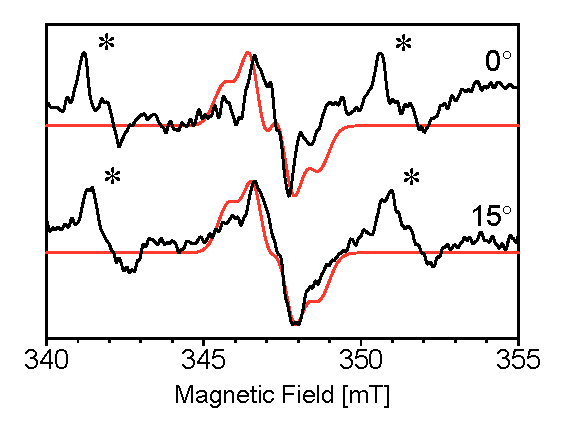
\includegraphics{Kapitel/Ch4-Images/03-PSII-xTal-Data.eps}
 \caption[Single-Crystal CW EPR of Y$_D^\bullet$ in photosystem II core complex.]{Single-Crystal continuous-wave EPR of Y$_D^\bullet$ in photosystem II core complex. Continuous-wave EPR collected with the 0.4~mm inner diameter self-resonant micro-helix at two angles of the photosystem II Y$_D^\bullet$ radical from a single crystal at a temperature of 80~K. The crystal size was 0.3 $\times$ 0.18 $\times$ 0.18~mm$^3$. Shown in red is a fitted simulation with similar features. A non-specifically bound Mn$^{2+}$ signal is also present in the mother-liquor of the crystal, indicated by an asterisk (\mbox{\large $\ast$}). Each spectrum was collected in 49 minutes with a signal-to-noise ratio of approximately 35.}
 \label{fig:xTalPSII}
\end{figure}

The use of photosystem II crystals as a benchmark provides a challenging system to measure. The photosystem II core complex has a molecular weight of approximately 455~kDa as a monomer and each complex contains only one Y$_D^\bullet$ radical. With a crystal size of 0.3 $\times$ 0.18 $\times$ 0.18~mm$^3$, a known average size of the unit cell, and that there are 8 photosystem II complexes per unit cell, one can calculate approximately 8.9$\times10^{12}$ Y$_D^\bullet$ radicals to be present in the sample. This demonstrates the versatility of the micro-helix to study large complexes in small crystal dimensions. A photosystem II core complex crystal can be routinely grown to dimensions of 0.3~mm, but requires significant effort to increase in size. Finally, the Y$_D^\bullet$ radical is easily saturable with large microwave magnetic fields, which limits the available microwave power and maximum EPR signal at a given temperature. Despite these challenges, a signal-to-noise of approximately 35 is calculated for the Y$_D^\bullet$ radical. 

\section{Conclusions and Outlook}
An application of the self-resonant micro-helix geometry and planar-coupling structure that increases the EPR absolute spin sensitivity by a factor of approximately 28 if the signal is unsaturable and 6 if the EPR signal is able to be saturated is presented. For saturable EPR signals, such as those found in protein samples, the self-resonant micro-helix saves up to a factor of 32 in measuring time. From this gain in sensitivity, the self-resonant micro-helix is well-suited for EPR studies on protein single-crystals with dimensions less than 0.3~mm. Due to the very high efficiency parameter of 3.2~mT/W$^{1/2}$, which corresponds to a $\pi/2$ pulse of 20~ns with an incident power of 20~mW, the micro-helix geometry is advantageous in extending pulse EPR to experiments that usually require costly high-powered microwave amplifiers (e.g. HYSCORE), further expanding the applicability of pulse EPR. We also show that the micro-helix performs well for field-swept non-adiabatic rapid scan (NARS) techniques due to its small size and ``open'' structure, which increases the continuous-wave EPR spin sensitivity further by a factor of 2 for the same experimental time. Due to the relatively large bandwidth of the micro-helix (90~MHz critically-coupled), this geometry is particularly well-suited for frequency-swept NARS and rapid scan experiments which further improve the signal-to-noise ratio for saturable samples\cite{Hyde2013MDIFF, MOSER2017} and for the use of arbitrary-waveform generators for advanced pulse spectroscopy. \cite{schweiger2001principles, chirpedESEEM, goldfarb2018epr}

The micro-helix Q-value and high efficiency parameter $\Lambda_{ave}$ of make the resonator suitable for watching the onset of the EPR signal during pulses. This resonator may allow us to approach ``dead-time free'' EPR for FID excitation. For example, if we assume a typical pulse X-band bandwidth of 70~MHz and a $Q_0$-value of 1000, a $\beta$ of 6.5 is needed to over-couple the cavity to the desired bandwidth. If we also assume it takes 15 time constants (factor of 2 for voltage detection) for the ring-down of the cavity 
\begin{equation}
    15 \time \tau_c = 15 \times 2 \times Q / 2 \pi \nu
\end{equation}
where $\nu$ is the frequency of interest. This produces a dead-time of 67~ns. For the micro-helix, with a critically-coupled measured $Q_0$-value of 220 the dead-time is 55~ns. (While critically-coupled, the signal-to-noise is improved by a $\sqrt{2}$ compared to an over-coupled cavity.) If we assume we can over-couple the micro-helix by a $\beta$ of 6.5, this leads to a dead-time of 15~ns. However, compared to the Bruker MS3, the micro-helix would need a factor of 10 less power for the same B$_1$, lowering the number of time constants needed.

As this technology matures, further improvements to enhance the sensitivity based on new fabrication techniques and choice of other materials will be explored. Not only does the increase in sensitivity save time in EPR data measurements, but also reduces the need of the availability of, or necessity to, grow larger crystals. Overall, the self-resonant micro-helix provides the possibility to study catalytically-active proteins at crystal dimensions relevant to X-ray crystallography and, as such, is a significant advancement in the field of enzyme research. 

{\renewcommand{\bibsection}{\clearpage\section*{\bibname}\markboth{\bibname}{\bibname}}
\renewcommand{\bibname}{CHAPTER 5. REFERENCES}
\bibliographystyle{elsarticle-num}
\bibliography{Kapitel/Ch5-References}
}

\chapter[Single-Crystal EPR on FeFe-Hydrogenase]{Single Crystal EPR on FeFe-Hydrogenase\blfootnote{Portions of this text are from J.~W.~Sidabras, J.~Duan, M.~Winkler, T.~Happe, R.~Hussein, A.~Zouni, D.~Suter, A.~Schnegg, W.~Lubitz, E.~J.~Reijerse, Sci. Adv., {\em accepted}.}}

Nature has evolved enzymes with various metallic cofactors (metallo-enzymes) to efficiently catalyze energy conversion reactions. These enzymes, which include, for example, photosystem II oxygen evolving complex\cite{CoxOEC}, hydrogenases\cite{lubitzhyd}, nitrogenases\cite{Hoffman2014rev}, and CO dehydrogenase\cite{C5CS00182J}, employ first-row transition metals to perform their catalytic functions. One of the main challenges is to fully understand these enzymatic mechanisms and provide a basis for cheap, robust, and highly active molecular catalysts designed for practical applications. \cite{Lewis15729} The ultimate goal is to alleviate the requirement of noble metals, such as platinum, that limit the scalability of current technology. This important biophysical and biochemical research seeks metallo-enzyme based and inspired systems as an interesting route to advance towards the future of clean energy and efficient energy storage. \cite{schlogl2012chemical}

The catalytic cycle of redox enzymes often contain paramagnetic intermediates and EPR is the method of choice used to study these occurrences. Through EPR experiments, information on the magnetic and geometrical structure of the active site can be obtained. EPR spectroscopy can probe isolated intermediates in the catalytic cycle when either a single unpaired electron or multiple unpaired electrons with magnetic couplings are present in the ground state. Fundamentally understanding such enzymes is of broad biochemical and biophysical importance as we move towards bioengineering mimics of nature’s most elusive chemistry. \cite{WATANABE20171}

One such interesting class of metallo-enzymes are the hydrogenases which catalyze the conversion of molecular hydrogen H$_2$, such that,
\begin{equation}
    \text{H}_2 \rightleftharpoons 2 \text{H}^+ + 2\text{e}^{\text{-}}.
\end{equation}
Hydrogenases are key enzymes in many organisms for hydrogen metabolism regulation in the cell or are used as electron donors for processes further down energy conversion pathways. The hydrogenase enzyme family has three distinct active-sites with different mechanistic hydrogen conversion. These mechanisms utilize either an single-iron center [Fe], a bi-nuclear iron [FeFe], or a nickle-iron [NiFe] active-site for catalysis. \cite{LubitzNiFe2016, lubitzhyd} 

Of great interest is the bi-nuclear [FeFe]-hydrogenase. \cite{PETERS20151350} These enzymes are amongst the fastest on the planet (turn-over frequencies over 10,000 s$^{\text{-1}}$ \cite{CatalyticTOF}) and provide a potential route to sustainable hydrogen production. The proposed crystal structure of one such hydrogenase from {\em Clostridium pasteurianum} (CpI) highlighting the active site and electron-transfer pathway is shown in Fig.~\ref{fig:CpIGeo}A. The electron-transfer pathway involving accessory iron-sulfur clusters is indicated as a solid blue arrow. In CpI, a [2Fe2S] cluster is found symmetric to the electron-transfer pathway, illustrated as a dashed blue line, and is believed to ``tune'' the redox potentials of the [4Fe4S] clusters. \cite{PetersPotentials} The [FeFe]-hydrogenase active-site carries a [4Fe4S] cluster linked via a cysteine ligand connecting the [2Fe]-cofactor molecule. The [2Fe]-cofactor contains an iron atom proximal (Fe$_p$) and one distal (Fe$_d$) to the [4Fe-4S] cluster. Each iron carries a cyanide (CN$^-$) and one carbonmonoxide (CO) ligand and the two irons share a bridging carbonmonoxide ($\mu$CO). Additionally, the two iron atoms are bridged by an azapropane-dithiolate-ligand (ADT-ligand). The molecular structure of the [FeFe]-hydrogenase active site, known as the H-cluster, can be found in Fig.~\ref{fig:CpIGeo}B. The whole active site has a total of six iron atoms at various redox states in the catalytic cycle. In the vicinity of the H-cluster, there exists proton (2H$^+$; illustrated as a dashed red line) and molecular hydrogen (H$_2$; illustrated as a solid red line) channels for gas exchange. Through many spectroscopic techniques, such as, Fourier Transform Infra-Red (FTIR), EPR, Nuclear Magnetic Resonance (NMR), M\"o\ss{}bauer, Raman, and Nuclear resonance vibrational (NRVS), a convincing catalytic cycle has been hypothesized. \cite{lubitzhyd, NRVS2017, sommer2017} However, more work must be done to fully understand the catalytic mechanism and relate it to quantum chemical calculations. 

\begin{figure}[htpb]
\centering
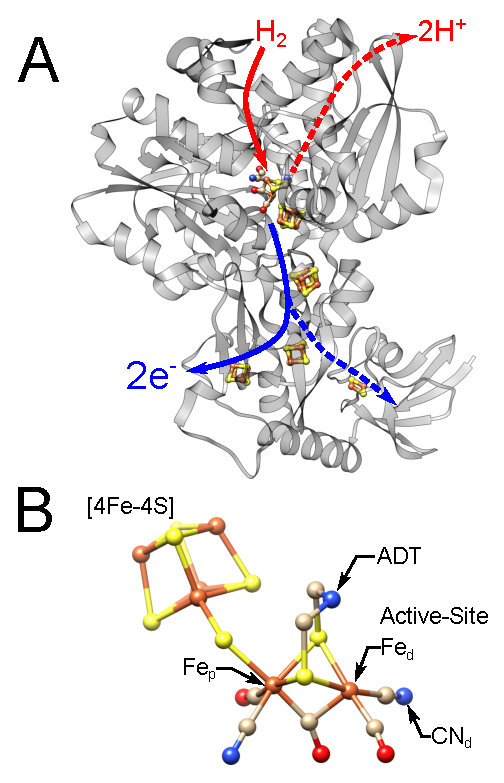
\includegraphics{Kapitel/Ch1-images/CpI-geometry.eps}
\caption[Crystal structure of {\em Clostridium pasteurianum} (CpI).]{A) Crystal structure of {\em Clostridium pasteurianum} (CpI) from PDB ID 4XDC. The [Fe-Fe]-Hydrogenase CpI is a 64~kDa protein with four [4Fe4S] clusters and one [2Fe2S] cluster. The iron-sulfur  clusters  are involved  in  the electron\-/transfer  pathway (solid blue). A [2Fe2S] cluster is found symmetric to the [4Fe4S] pathway (dashed blue) and is believed to ``tune'' the redox potentials of the nearby [4Fe4S] clusters. There exists a proton (2H$^+$;dashed red) and hydrogen (H$_2$; solid red) channel for gas exchange. The active-site, or H-cluster, resides at the top in this view and is B) expanded to show the H-cluster structure. Within the H-cluster, the proximal iron (Fe$_p$) and distal iron (Fe$_d$) of the [FeFe]-hydrogenase is shown. In this view, Fe is orange, S is yellow, N is blue, O is red, and C is beige.}
 \label{fig:CpIGeo}
\end{figure}

Using frozen solution samples, EPR spectroscopy has been used to study the paramagnetic states of [FeFe]-hydrogenase from a number of organisms. \cite{lubitzhyd,Silakov57Fe,Adamska2015pdt,Adamska2015} These experiments have determined the magnetic principal \textit{g}-values, hyperfine, and quadrupole parameters for the catalytic states with EPR active co-factors and [4Fe4S] clusters. Such important intermediate states include H$_{ox}$ and H$_{sred}$ in the catalytic cycle, a reversible carbon monoxide (CO) inhibited H$_{ox}$-CO state, and any state with reduced [4Fe4S] clusters, including the \textit{apo}-HydA protein which lacks the H-cluster. In this work we focus on H$_{ox}$ which is the primary catalytic state of the [FeFe]-hydrogenase.

It was found that an {\em Escherichia coli} ({\em E. coli}) expressed \textit{apo}-HydA could be combined with an artificially synthesized H-cluster to form fully functional [FeFe]\-/hydrogenase. \cite{EsselbornArtificial, BirrellArtificial} This has not only increased the yields of the precursor of the binuclear co-factor but has allowed synthetically modified co-factors to be inserted and a wealth of information has been obtained, including the identification of the head group in the bridging ADT-ligand. \cite{AdamskaBridgingAmine} With this tool, it became possible to enrich the H-cluster with magnetic isotopes and study the corresponding magnetic interactions. These experiments allowed the synthesis of $^{57}$Fe in the binuclear  co-factor, $^{13}$C, $^{14}$N, and $^{15}$N in the CN$^-$ and ADT ligands, and $^{13}$C in the CO ligands. A summary of the magnetic properties of the H$_{ox}$ state can be found in Table~\ref{table:eprthing}. 

\begin{table}[hb]
\caption[EPR parameters determined for FeFe-hydrogenase in Hox state.]{EPR parameters determined by frozen solution of [FeFe]-hydrogenase in the H$_{ox}$ state through a series of pulse EPR experiments.}
\centering
\begin{tabular}{l|c|c||c}
 & Fe$_p$ $^\dagger$ & Fe$_d$ $^\dagger$ & {[}4Fe4S{]} \\ \hline \hline
oxidation state & II & I & 2+ \\
Spin state & $S=0$ & $S=1/2$ & $S_{eff}=0$ \\
$g$-values & -- & {[}2.100, 2.040, 1.999{]} & -- \\
A (MHz) & {[}12.3, 11.4, 12.6{]} & {[}12.3, 11.4, 12.6{]} & $\pm${[}11.2, 10.4, 11.6{]} \\
{[}$\alpha$, $\beta$, $\gamma${]} (deg) & {[}0, 0, 0{]} $\pm$30 & {[}0, 0, 0{]} $\pm$30 & {[}0, 0, 0{]} $\pm$30
\end{tabular}
\begin{flushleft}\footnotesize{$^\dagger$ From DFT calculations of Ref.~[1.\kern-0.4em\citenum{GrecoDFT}], we assume the majority of the spin is located on Fe$_d$; however, significant $^{57}$Fe hyperfine interactions on both irons are measured by Silakov {\em et al.} in Ref.~[1.\kern-0.4em\citenum{Silakov57Fe}].} \end{flushleft}

\begin{tabular}{l|c|c|c}
& C$^{15}$N$_d$ $^\ddagger$ & C$^{14}$N$_d$ $^\ddagger$ & ADT-Ligand ($^{14}$N)$^{\ddagger^\ddagger}$\\ \hline \hline
A (MHz) &  {[}-1.3, -1.1, 6.2{]} & {[}-0.9, -0.8, 4.4{]} & {[}1.35, 1.15, 1.15{]}\\
{[}$\alpha$, $\beta$, $\gamma${]} (deg) & {[}-90, -50, 0{]}$^\ast$ & {[}-90, -50, 0{]}$^\ast$ & {[}0, 0, 0{]}\\
$P_{||}$ {[}MHz{]} &  -- & 0.9 & 1.23\\ 
$\eta$ & -- & 0.34 & 0.13 \\
{[}$\alpha$, $\beta$, $\gamma${]} (deg) & -- & {[}-46, -119, 0{]}$^\ast$ & {[}0, -90, 0{]}$^\ast$
\end{tabular}
\begin{flushleft}\footnotesize{$^\ddagger$ Data is obtained from Adamska {\em et al.} of Ref.~[1.\kern-0.4em\citenum{Adamska2015}]. Other groups, such as Britt and colleagues in Ref.~[1.\kern-0.4em\citenum{BrittLigands2014}] have obtained similar values; however, Adamska {\em et al.} use the same molecular frame described in this work. 

$^{\ddagger^\ddagger}$ Data is obtained from Adamska {\em et al.} of Ref.~[1.\kern-0.4em\citenum{Adamska2015pdt}]. 

$^\ast$ The Euler angles are in the new EasySpin Euler definition (since version 5.0), which required the transformation $[\alpha,\beta,\gamma]= -[\gamma,\beta,\alpha]$ from the published results.} \end{flushleft}

\begin{tabular}{l|c|c}
 & $^{13}$CN$_p$ $^\ddagger$ & $^{13}$CN$_d$ $^\ddagger$  \\ \hline \hline
A (MHz) & {[}5.52, 5.52, 4.55{]} & {[}30, 28.5, 22.7{]} \\
{[}$\alpha$, $\beta$, $\gamma${]} (deg) & {[}0, 0, 0{]}  \\
\end{tabular}
\begin{tabular}{l|c|c|c}
 & $^{13}$CO$_p$$^{\ast\ast}$ & $^{13}$CO$_d$$^{\ast\ast}$ & $\mu^{13}$CO$^{\ast\ast}$ \\ \hline \hline
A (MHz) & {[}5.52, 5.52, 4.55{]} &  {[}20.5, 29.9, 26.0{]} & {[}9.0, 3.8, 4.5{]}\\
{[}$\alpha$, $\beta$, $\gamma${]} (deg) &  {[}25, 25, 0{]} & {[}37, 26, 0{]} & {[}0, 20, 0{]} \\
\end{tabular}\label{table:eprthing}

\begin{flushleft}\footnotesize{$^{\ast\ast}$ Data is obtained from Britt {\em et al.} of Ref.~[1.\kern-0.4em\citenum{BrittC13}].} \end{flushleft}
\end{table}

The data in Table~\ref{table:eprthing} represents the current knowledge on the magnetic properties of the [FeFe]-hydrogenase in the H$_{ox}$ state. However, this table is not exhaustive and further information on both the magnitude and orientation of the \textit{g}-, hyperfine-, and quadrupole-tensors is still needed. To date, quantum chemical calculations have difficulties in predicting the principal values of the \textit{g}-tensor\cite{GrecoDFT, FiedlerDFT} and are only used to qualitatively assign spin densities when simulating interactions with surrounding nuclei. From the current literature, it is not clear on what amino acids are involved in the first ligand-sphere and, therefore, single crystal EPR experiments are needed to properly determine the full-magnetic interactions of the H-cluster. 

In this work, advancement to the state-of-the-art EPR instrumentation is achieved in order to improve both frozen solution data acquisition methods and obtain the ability to measure protein single crystals with dimensions less than 0.3~mm$^3$. From the EPR single crystal data, past studies using assumptions and speculations of the \textit{g}-tensor and how it relates to the surrounding nuclei can be refined or abandoned; while, quantum chemical calculations of the magnitudes and orientations of the magnetic tensors can be tested by comparing to experimental data.

Using the photosystem II Y$_D^\bullet$ radical in Chapter~5, we have established that the self-resonant micro-helix is suitable for studies of single-crystal protein samples of volumes less than 27~nL. The self-resonant micro-helix is optimal for these experiments due to the relatively large bandwidth (90~MHz critically-coupled), efficiency of 3.2~mT/W$^{1/2}$, which corresponds to a $\pi/2$ pulse of as short as 20~ns with an incident power of only 20~mW, and the relatively homogeneous microwave magnetic field incident on the sample. We now want to demonstrate that i) a full angular $g$-tensor determination can be performed and, due to the six fold signal enhancement, that ii) advanced pulse EPR experiments, like ESEEM and HYSCORE, in single crystals are not only feasible, but useful. 

We report here, for the first time, a proposed $g$-value from field-stepped ESE rotational data and HYSCORE derived data for a [FeFe]-hydrogenase in the active oxidized state (H$_{ox}$) from {\em Clostridium pasteurianum} in a 0.3 $\times$ 0.1 $\times$ 0.1~mm$^3$ crystal volume. These data demonstrate the utility of the micro-helix in studying protein single-crystals at sizes relevant for X-ray crystallography.

\section{Methods}
The [FeFe]-hydrogenase from {\em Clostridium pasteurianum} (CpI) was grown and crystallized to a size of 0.3 $\times$ 0.1 $\times$ 0.1~mm$^3$ by the method of Esselborn {\em et al.}\cite{FeFeCry} under auto-oxidative conditions, i.e. without reducing agents. This leaves the enzyme in the characteristic active oxidized state (H$_{ox}$), giving rise to a $S=1/2$ ground state of the H-cluster. The accessory iron-sulfur clusters in the protein are oxidized and remain EPR silent. \cite{lubitzhyd}  Under a microscope in an anaerobic chamber, the protein crystal is drawn by capillary action into a 0.3~mm inner diameter capillary with mother liquor and cryoprotectant, centered in the micro-helix, and flash frozen. The micro-helix assembly is affixed to the EPR probehead, placed in a pre-cooled cryostat, and attached to the EPR bridge. The whole micro-helix probehead is then rotated in 5$^{\circ}$ steps over 180$^{\circ}$ in one-plane within the magnet. 

\begin{figure}[htbp]
\centering
 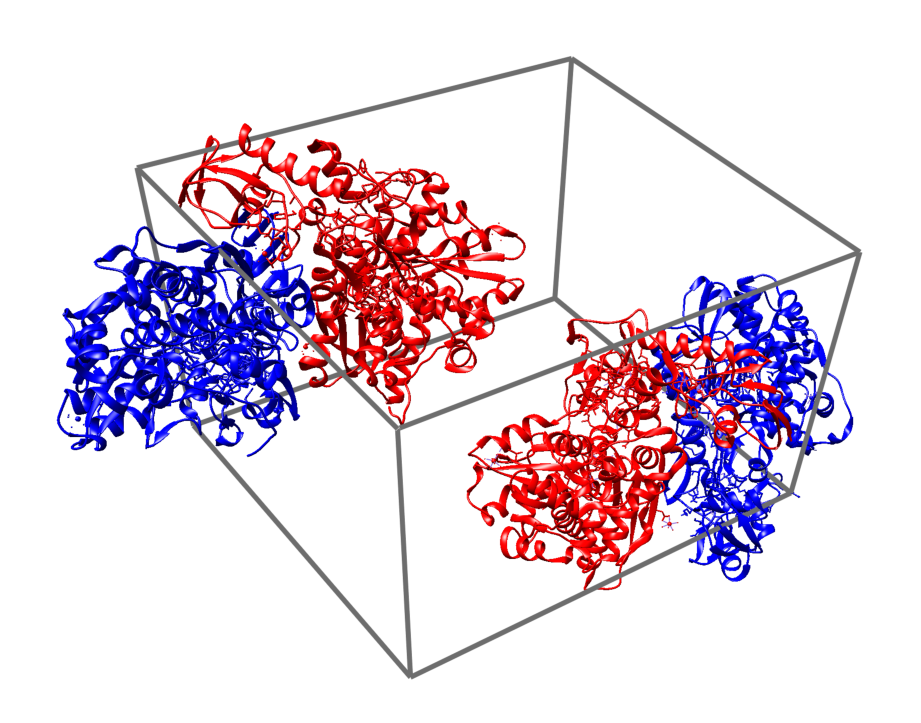
\includegraphics[width=0.5\textwidth]{Kapitel/Ch6-Images/Ch6-UnitCell.eps}
 \caption[Unit Cell from PDB 4XDC.]{Shown is the unit cell of PDB ID 4XDC with the molecules in an asymmetric unit (red and blue) and copied by the P$1\,2_1\,1$ symmetry.} 
 \label{fig:xTalFeFeUnit}
\end{figure}

The [FeFe]-hydrogenase of {\em Clostridium pasteurianum} (CpI) has a molecular weight of 67~kDa. The unit cell has P$1\,2_1\,1$ symmetry with two molecules in the asymmetric unit (PDB ID: 4XDC), shown in Fig.~\ref{fig:xTalFeFeUnit}. Each of the four enzymes per unit cell contain one active-site (H-cluster, shown in Fig.~1.1B in Chapter~1) which results in four distinct signals. The single crystal had a volume of approximately 0.3 $\times$ 0.1 $\times$ 0.1~mm$^3$ and, based on the unit cell dimensions, approximately 17$\times10^{12}$ enzymes within the crystal are calculated. The four observed signals corresponding to 4.25$\times10^{12}$ spins per peak. 

In the current setup, the entire probe head is rotated within the magnet with the static magnetic field in the laboratory frame $L_1$-direction and rotation takes place on axis of the microwave magnetic field in the $L_3$-direction, per Fig.~2.6A in Chapter 2. Since the setup is axially symmetric, this allows for full rotation in one crystal plane over 180 degrees. The laboratory frame is set in the EasySpin simulations and the collected spectra are fitted using the Matlab programs supplied in Appendix~3 or at: https://act-epr.org/data. The \textit{esfit} routine was modified with a sub-routine employing partial parallelization of the simulations. This allowed for 12 spectra in 3 chunks to be simulated simultaneously for a total of 36 spectra per fit. A particle swarm optimization algorithm with 10,000 particles (fits) was used to find the solution. Each run was allowed to converge in 10 iterations and checked if a local minimum was found. The Easyspin solution took about 1~second for each fit for a total of approximately 2.5~hours per iteration. Simulations were re-run until a good fit was established.

The simulation is setup with 9 unknowns: the three axes of the crystal frame that relates how the crystal is orientated in the laboratory frame, the three axes of the g-tensor of the first molecule (g-Tensor A) and how it relates to the Molecular-Frame A, and the three axes of the g-tensor of the second molecule (g-Tensor B) and how it relates to the Molecular-Frame B. However, we can assume that the g-tensor of the second molecule will be almost the same as the first molecule, based on similar research at W-band with photosystem II. \cite{Hofbauer6623, B908093G} From this knowledge, we can limit the deviation of the $g$-tensor of the second molecule ($g$-tensor B) with respect to the first ($g$-tensor A). The crystal frame and $g$-tensor A were set to vary from a whole rotation. We assume that $g$-tensor B has minimal deviation from the solution of $g$-tensor A. Therefore we limited the $g$-tensor variation to only 15 degrees different compared to $g$-tensor A. The principal $g$-values were obtained from previous frozen solution EPR experiment in Ref.~[6.\kern-0.4em\citenum{lubitzhyd}] ($g$-values: [1.999, 2.039, 2.097] corresponding to $x$, $y$, and $z$, respectively).

The HYSCORE experiment has a ${\pi/2\!-\!\tau\!-\!\pi/2\!-\!t_1\!-\!\pi\!-\!t_2\!-\!\pi/2}$ pulse sequence which results in an echo $\tau$ seconds after the last $\pi/2$ pulse. The values for $t_1$ and $t_2$ are swept to form a 2D experiment at a fixed magnetic field position. Herein, the magnetic field is set to one of the peaks measured in the two-pulse ESE experiment, $\tau$ is 280~ns, $t_1$ and $t_2$ start at 300~ns with 256 48~ns steps, and $\pi$-pulse is 80~ns at a microwave power of 7~mW. 

\section{Results and Discussion}
\subsection{Pulse EPR in Single Crystals of [FeFe]-Hydrogenase.}
\begin{figure}[htbp]
\centering
 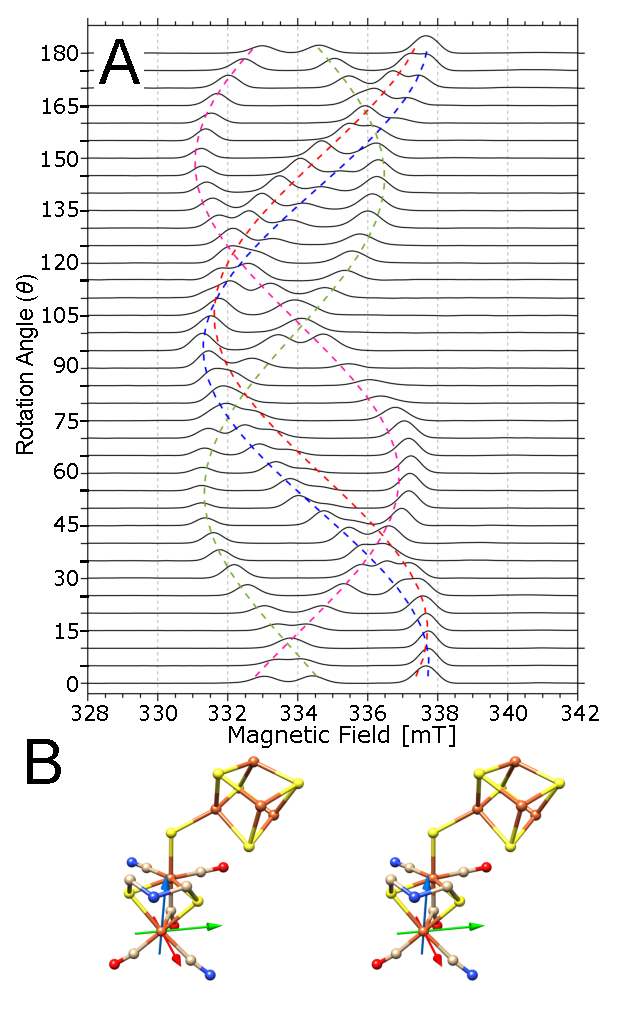
\includegraphics{Kapitel/Ch5-Images/04-FeFe-xTal-DataBig.eps}
 \caption[Pulse EPR on single-crystal of the H-cluster in FeFe-hydrogenase.]{A) Pulse EPR on single-crystal [FeFe]-hydrogenase of {\em Clostridium pasteurianum} (CpI) in the H$_{ox}$ state showing collected data in one plane for a full rotation of 180$^{\circ}$ in 5$^{\circ}$ steps at a temperature of 15~K. B) A stereo view of the analyzed $g$-tensor (g$_x$: green, g$_y$: blue, g$_z$: red) is mapped on the crystal structure (PDB ID: 4XDC). We assume that the order of the principal values of the $g$-tensor is $g_z\geq g_y\geq g_x$. For a 3D view of the proposed $g$-tensor see: https://act-epr.org/FeFeHydrogenase.html} 
 \label{fig:xTalFeFe}
\end{figure}

First, a field-swept two-pulse electron spin-echo EPR experiment was performed every 5$^{\circ}$ on a protein single-crystal of the [FeFe]-hydrogenase of {\em Clostridium pasteurianum} (CpI) in the oxidized H$_{ox}$ state and plotted in Fig.~\ref{fig:xTalFeFe}A. A very good signal-to-noise ratio of approximately 290 is calculated for a collection time of 8~minutes for each spectrum at a temperature of 15~K. 

From these spectra, the data can be fitted to simulations which relate the different frames of reference to each other as defined in the EasySpin simulation package. Rotational matrices for the relationship of these frames can be found in Table~\ref{table:frames}. The rotational matrices are found from the Euler angles found from the fitting of the laboratory and $g$-tensor frames. The resonance roadmap is overlaid on the field-swept two-pulse electron spin-echo EPR experiment shown in Fig.~\ref{fig:xTalFeFe}A. A second experiment with the same crystal was peformed and can be found in Appendix D Figs.~D.1 and D.2. The measurement in the second plane provides confidence in the fit of the $g$-tensor. A very good fit in both experiments was found. 

\begin{table}[ht]
\caption[Rotational matrices for the crystal frame.]{Rotational matrices  for the crystal frame with respect to the laboratory frame and the $g$-tensor with respect to the molecular frame. The crystal frame and $g$-tensor are found by fitting the data in Fig.~\ref{fig:xTalFeFe}A with the molecular frame from PDB ID 4XDC.}
\centering
\hspace{-12.825em}
\begin{tabular}{r|ccc}
 & \multicolumn{3}{c}{Crystal Frame} \\
\multicolumn{1}{l|}{} & $a$ & $b$ & $c$ \\ \hline \hline
L$_1$ & $+$0.273 & $-$0.162 & $-$0.948 \\
L$_2$ & $-$0.022 & $-$0.987 & $+$0.162 \\
L$_3$ & $-$0.962 & $+$0.023 & $-$0.273
\end{tabular}\label{table:frames} \\
\vspace{0.5cm}
\begin{tabular}{r|ccc|ccc}
 & \multicolumn{3}{c|}{Molecular-Frame A} & \multicolumn{3}{c}{Molecular-Frame B} \\
 & $x$ & $y$ & $z$ & $x$ & $y$ & $z$ \\ \hline \hline
$a$ & $-$0.331 & $-$0.938 & +0.107 & $-$0.595 & $-$0.666 & $-$0.450 \\
$b$ & $-$0.770 & +0.203 & $-$0.605 & +0.456 & $-$0.740 & +0.494 \\
$c$ & +0.545 & $-$0.283 & $-$0.789 & $-$0.662 & +0.089 & +0.744
\end{tabular}\\
\vspace{0.5cm}
\begin{tabular}{r|ccc|ccc}
 & \multicolumn{3}{c|}{\textit{g}-Tensor A} & \multicolumn{3}{c}{\textit{g}-Tensor B} \\
 & $x$ & $y$ & $z$ & $x$ & $y$ & $z$ \\ \hline \hline
$a$ & $+$0.476 & $-$0.484 & $+$0.735 & $+$0.377 & $-$0.605 & $-$0.701 \\
$b$ & $-$0.400 & $+$0.625 & $+$0.671 & $-$0.388 & $+$0.584 & $-$0.713 \\
$c$ & $+$0.783 & $+$0.613 & $-$0.103 & $+$0.841 & $+$0.541 & $-$0.015
\end{tabular}
\end{table}

The proposed $g$-tensor orientation is plotted as a stereo view in Fig.~\ref{fig:xTalFeFe}B. The $g$-tensor (g$_x$: green, g$_y$: blue, g$_z$: red) is presented with the origin at the distal iron (Fe$_d$), since Fe$_d$ is known to contain most of the spin density in the H$_{ox}$ state. \cite{FiedlerDFT,GrecoDFT} The $g$-tensor orientation found here is close to that proposed by Adamska {\em et al.} using HYSCORE measurements in frozen solution. \cite{Adamska2015} Direct comparison of the two proposed $g$-tensors can be found in Fig.~\ref{fig:gTensor}. 

Adamska {\em et al.} could simulate and calculate a hypothetical $g$-tensor that would give rise to the measured HYSCORE spectra. From this calculation, it was proposed that the g$_z$-axis lies along the Fe$_p$-Fe$_d$ axis in order to fit a CN$_d^-$-Fe$_d$-g$_z$ angle of 117$^\circ$ as shown in Fig.~\ref{fig:gTensor}A. The g$_x$-axis was chosen to point along the Fe$_d$ to ADT-amine nitrogen axis in order to bisect the nitrogen which is believed to be part of the formation of the hydride. The data collected using single-crystal EPR in this work is in good agreement with Adamska {\em et al.} and shows a deviation of only 10.1$^{\circ}$ from the axes previously proposed, shown in Fig.~\ref{fig:gTensor}B. However, the newly proposed $g$-tensor orientation has the $x$-axis pointing outward at the open coordination site and a 9.1$^{\circ}$ deviation from bisecting the H-cluster. These rotations cannot be found with frozen solution data and are only available with single-crystal experiments. No assumptions are made in the fitting of the $g$-tensor from single-crystal data. Further analysis and refinement is possible with the collection of hyperfine and quadrupole data originating from the same crystal and relating the whole dataset to quantum chemical calculations.

\begin{figure}[ht]
\centering
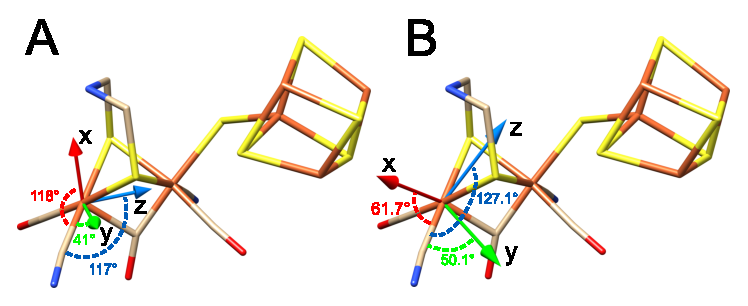
\includegraphics{Kapitel/Appendix/Images/S6-gTensorCompare.eps}
\caption[Comparison of the proposed $g$-tensor.]{A) The proposed $g$-tensor by Adamska {\em et al.} overlaid onto the H-cluster from PCB ID 3C8Y. (Adapted from Ref.~[6.\kern-0.4em\citenum{Adamska2015}] with permission from the PCCP Owner Societies.) B) The proposed $g$-tensor of this work overlaid onto the H-cluster from PCB ID 4XDC.}
\label{fig:gTensor}
\end{figure}

\subsection{Advanced Pulse EPR on the H-cluster in Single Crystals.}
Due to the excellent signal-to-noise of the field-stepped ESE we were able to perform single crystal ESEEM/HYSCORE experiments. HYSCORE was performed every 30$^{\circ}$ on each of the peaks shown in the field-swept ESE EPR dataset. Each spectrum was collected over approximately one hour, using a standard four-pulse HYSCORE sequence. \cite{schweiger2001principles} To obtain information on the hyperfine- and quadrupole-tensors, HYSCORE or ESEEM data must be collected on at least one peak and followed through a 180$^{\circ}$ rotation in order to obtain the axial relationship of the hyperfine interactions. Multiple peaks can be used to over-determine the system. A series of HYSCORE experiments following the fuchsia-colored resonance roadmap of Fig.~\ref{fig:xTalFeFe}A is shown in Fig.~\ref{fig:FeFeHYSCOREFollow}. 

\begin{figure}[ht]
\centering
 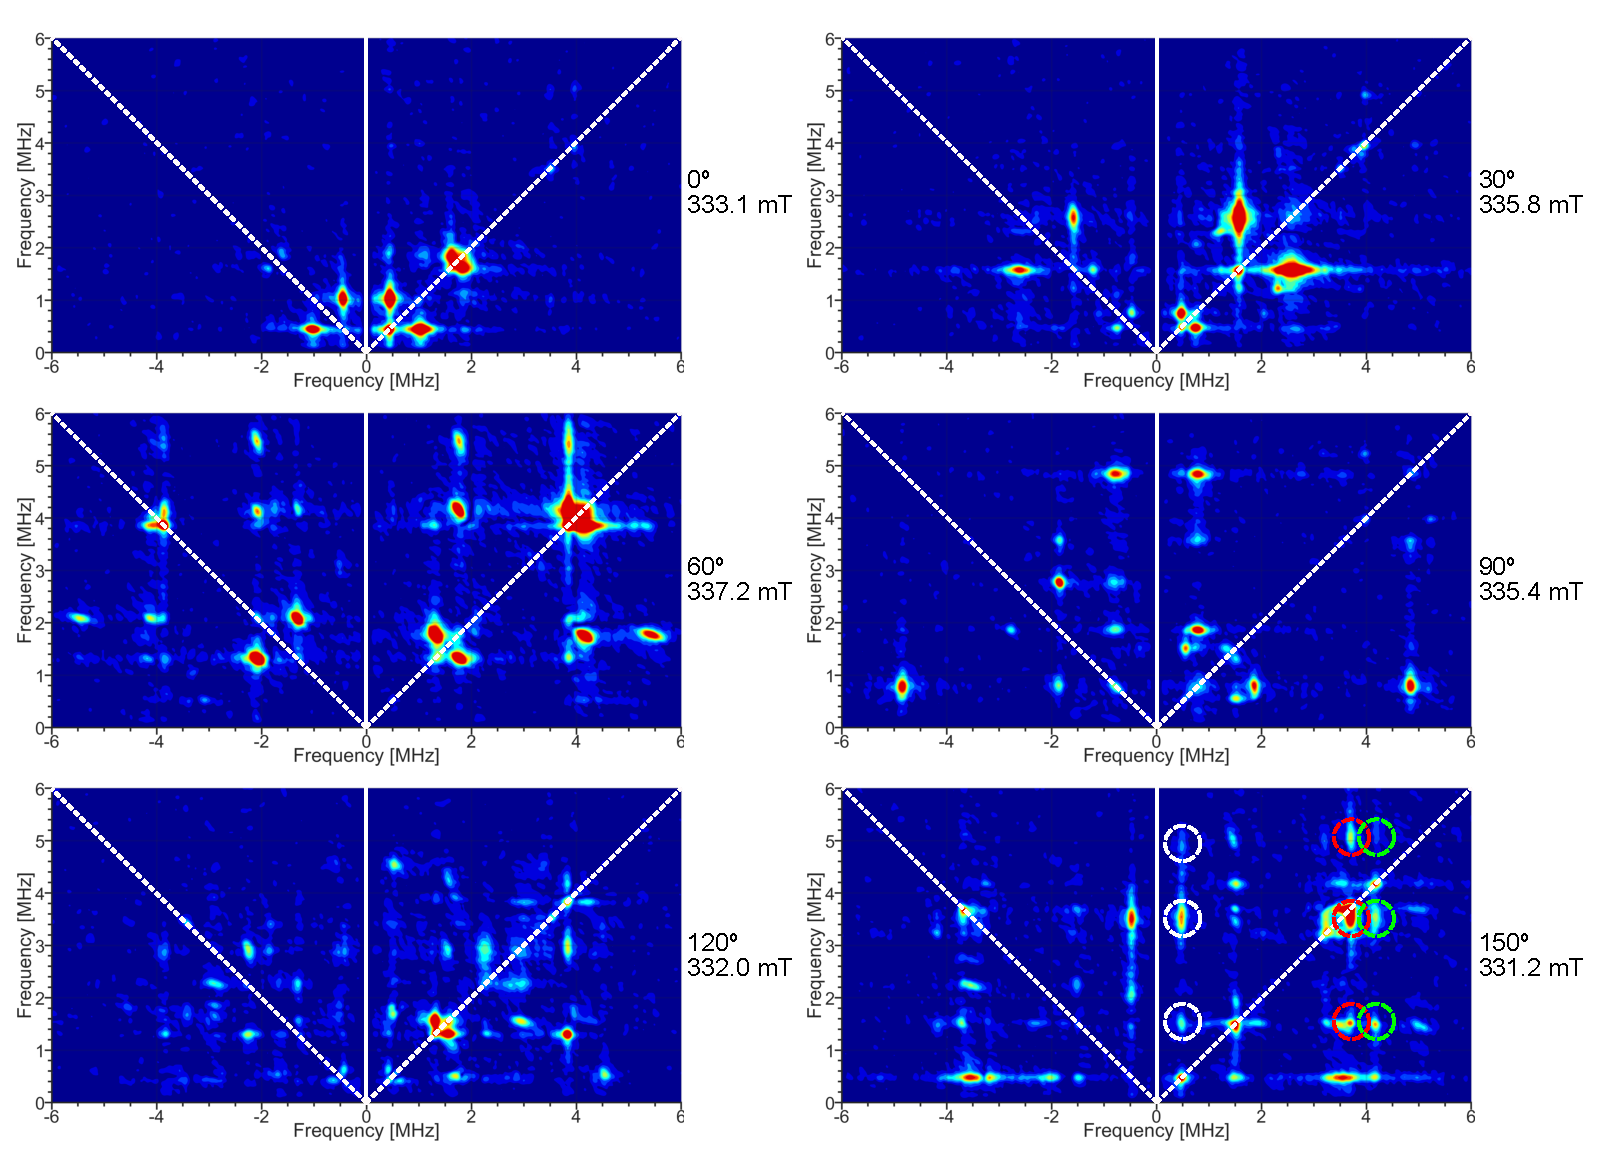
\includegraphics[width=\textwidth]{Kapitel/Ch5-Images/FeFe-FollowHyscore.eps}
 \caption[Single-crystal HYSCORE EPR following a single peak.]{Single-crystal HYSCORE EPR following the fuchsia-colored resonance roadmap of Fig.~\ref{fig:xTalFeFe}A.} \label{fig:FeFeHYSCOREFollow}
\end{figure}

In a HYSCORE experiment, the 2D density representation shows correlations between the nuclear-spin transitions (m$_\text{I}$) in both projections of the electron spin. Both, the $^{14}$N nucleus ($I=1$) from a distal cyanide-ligand (CN$_\text{d}^-$) and the secondary-amine group in the azapropane-dithiolate-ligand (ADT-ligand) can potentially contribute to the HYSCORE spectrum generating three transitions per ligand for each electron-spin transition (m$_\text{S}$) manifold for a maximum of 12 modulation frequencies. According to an earlier study on H$_{ox}$ in frozen solution, the features of the distal cyanide-ligand spread out up to 6 MHz, while the transitions of the ADT-amine nitrogen are found between 2 and 4~MHz. \cite{Adamska2015,Adamska2015pdt}

Currently, the full hyperfine- and quadrupole-tensor has not been solved. However, we can compare the data that was collected with previous work and gain further insight. For example, in Fig.~\ref{fig:FeFeHYSCOREFollow} at 0 and 30 degrees a strong signal can be seen in the weak coupling (++) quadrant under a coupling frequency of 4~MHz. These signals are attributed to the ADT-ligand and fit the principle values described in Adamska {\textit et al.} \cite{Adamska2015pdt} As the HYSCORE data is rotated these signals are reduced and signals with larger couplings are found in the 4 to 6~MHz range, including signals in the strong coupling ($-+$) quadrant. These signals are best represented by the distal cyanide-ligand (CN$_\text{d}^-$) as descrbed in a second paper by Adamska {\textit et al.} \cite{Adamska2015}.

A second data set of ESEEM was performed following the fuchsia-colored resonance roadmap of Appendix D Fig.~D.1 and plotted in Fig.~\ref{fig:ESEEM2}. These ESEEM data were performed at a finer resolution of 5 degree steps over 180 degree rotation. From this data we can 

\begin{figure}[ht]
\centering
 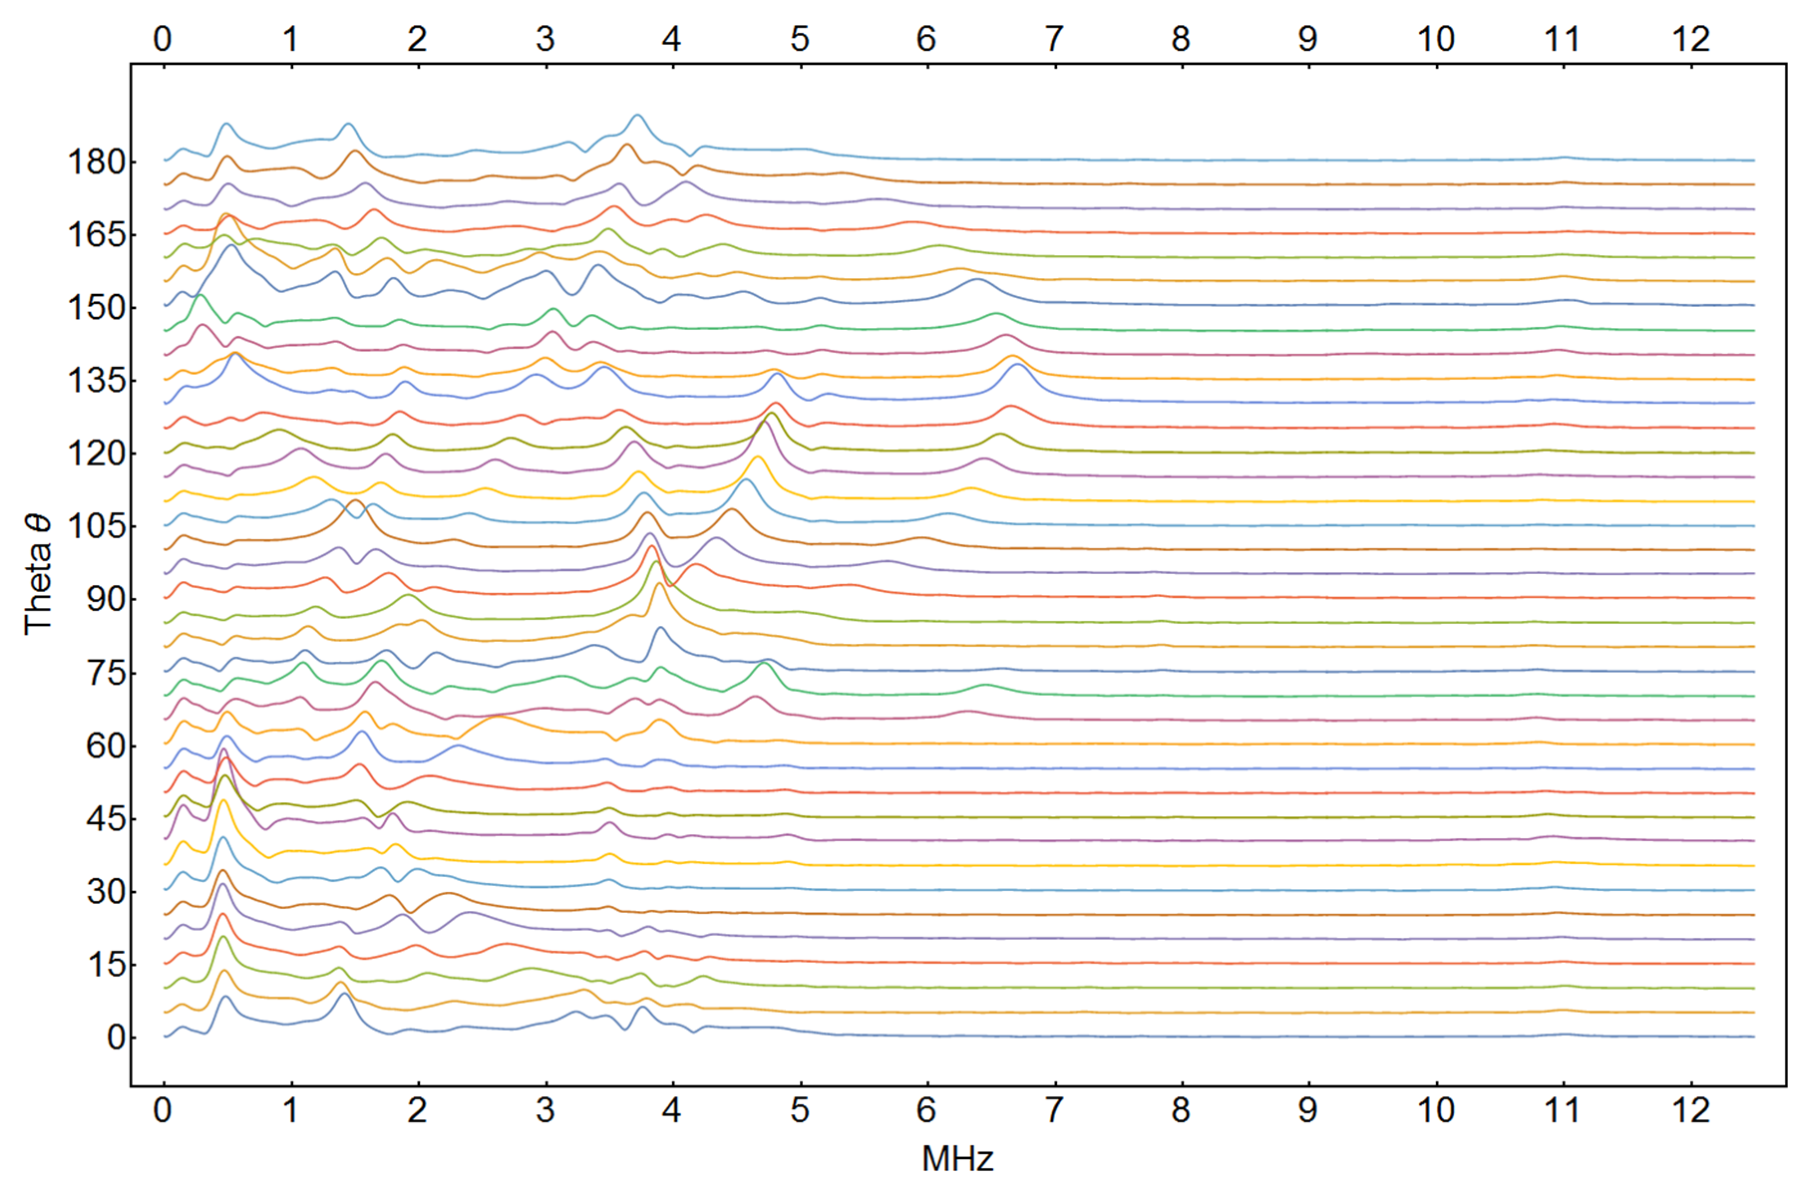
\includegraphics[width=0.8\textwidth]{Kapitel/Appendix/ESEEMFirstPeak.eps}
 \caption[Single-crystal ESEEM EPR: Fuchsia Trace.]{Single-crystal ESEEM EPR following the fuchsia-colored resonance roadmap of Fig.~D.1.} \label{fig:ESEEM2}
\end{figure}

\section{Conclusions and Outlook}
In this work we have demonstrated that a full angular $g$-tensor determination can be performed on crystals smaller than 27~nL volumes with excellent signal-to-noise at X-band. The proposed $g$-tensor is a refinement on previous work by Adamska {\em et al.}, which used orientation-selection HYSORE on frozen-solution samples at X-band and Q-band to back project the $g$-tensor. In this work, no assumptions are made and the $g$-tensor is measured directly. Although a single plane was rotated, the P$1\,2_1\,1$ symmetry of the crystal and the orientation of the crystal in the Laboratory Frame has allowed for a good fit. 

This work also demonstrates the ability to perform HYSCORE experiment on the same crystal and highlights the feasibility of such advanced EPR experiment. Future ESEEM/HYSCORE experiments will address the $^{14}$N couplings of the CN$^-$ and ADT ligands in greater detail. Possibly this will involve selective $^{15}$N labeling as has been demonstrated before. \cite{Adamska2015, AdamskaBridgingAmine} From such experiments, extracting the magnitude and orientation of the hyperfine- and nitrogen quadrupole-tensors in the molecular axis frame and relating these to the electronic structure as predicted through quantum chemical calculations are possible. 

\section*{Contributions} Jason W. Sidabras, Dr. Edward Reijerse, and Prof. Wolfgang Lubitz conceived the project. Jason W. Sidabras prepared all crystals for EPR experiments, performed the measurements, and analyzed the data. Within the group of Prof. Thomas Happe, Drs. Jifu Duan and Martin Winkler grew [FeFe]-hydrogenase crystals from {\em Clostridium pasteurianum} (CpI) in the H$_{ox}$ state. Dr. Reijerse was integral in setting up the EPR experiments and the discussion of the analyzed data. 


{\renewcommand{\bibsection}{\clearpage\section*{\bibname}\markboth{\bibname}{\bibname}}
\renewcommand{\bibname}{CHAPTER 6. REFERENCES}
\bibliographystyle{elsarticle-num}
\bibliography{Kapitel/Ch5-References}
}
\chapter[Summary and Future Work]{Summary and Future Work}
\setcitestyle{citesep={,\,\thechapter.}}

In this body of work, three challenges of modern EPR were addressed by the development of application-specific microwave resonant structures. These efforts span the frequency range from 9.5 to 420~GHz.

In Chapter 3, the introduction of the uniform field re-entrant TE$_{\text{01U}}$ resonator at Q-band frequencies (35~GHz) improves EPR sensitivity by providing more homogeneous $\pi/2$ and $\pi$ pulses incident on the sample. This has an advantage in pulse experiments with complex sequences used for excitation of the spin system. 

For example, HYSCORE data at Q-band will benefit from uniform magnetic field excitation by providing a mixing pulse which will maximize the nuclear transition mixing and remove on-diagonal signals. \cite{Doorslaer2007,Harmer2009} Such signals typically dominate the spectrum and make interpretation difficult. For EDNMR, a uniform magnetic field excitation translates into a reduction of the width of the central peak allowing for the measurement of modulation frequencies typically hidden by this feature. \cite{NicholasCox2013} Finally, the increase in resonator bandwidth, from the lower Q-value and implementation of a more efficient waveguide junction, allows the spectroscopist to utilize state-of-the-art arbitrary waveform generators for further signal improvement and method development. \cite{DOLL201327,dSegawa2015,SPINDLER201730,WILI201826,PRISNER201998}

In Chapter~4, the experiments in the THz-bandgap with hemin sample and meta-materials made from an array of split-ring resonators at 420~GHz serve as an interesting example of the two oscillator problem in physics. Using analytical lumped-circuit transmission-line theory, the EPR response was fully reproduced. The use of split-ring resonators creates a cross-sectional area that is not limited by the wavelength of the operating frequency. The split-ring resonators maintain an active depth proportional to the individual geometry providing a suitable volume for thin-film samples. An EPR signal enhancement is measured at the operating frequency of the split-ring resonators. With the new understanding outlined in this work, it may be possible to design a series of multi-frequency high-field EPR experiments with meta-material resonant discs at each frequency. This will allow spectroscopists to probe the zero-field splitting characteristics of high-spin samples in thin films or limited samples.

The introduction of the self-resonant micro-helix at X-band (9.5~GHz) in Chapter~5 provides a resonator efficiency of 3.2~mT/W$^{1/2}$ corresponding to a $\pi/2$ pulse of 20~ns with an incident power of only 20~mW. The self-resonant micro-helix exhibits an absolute sensitivity increase up to a factor of approximately 30 in the EPR signal compared to commercial resonators. For samples that saturate readily, the micro-helix provides a factor of 6 in absolute EPR sensitivity improvement compared to commercial resonators. This translates into a factor of 36 in measurement time for equivalent sample volumes. Additionally, the high resonator efficiency and low $Q_0$-value (bandwidth of 90~MHz critically coupled) provides an opportunity to measure FID induced EPR on systems without costly high-power amplifiers, further extending the usefulness of pulse EPR spectroscopy.

Finally, the implementation of the self-resonant micro-helix has allowed, for the first time, the collection of EPR data from a 0.3 $\times$ 0.1 $\times$ 0.1~mm$^3$ single crystal of [FeFe]-hydrogenase in the H$_{ox}$ state from {\em Clostridium pasteurianum} (CpI). Full $g$-tensor analysis was successfully performed and a proposed orientation of the principal axes is discussed. With the excellent signal-to-noise ratio, data was also collected on the same protein crystal using an ESEEM/HYSCORE pulse sequence. These data show an angle dependant $^{14}$N hyperfine- and quadrupole-tensor originating from either the cyanide-ligand of the distal iron or the ADT-ligand.  To our knowledge, the ESEEM/HYSCORE spectra collected herein are the first published results from a protein single-crystal with a volume of 3~nL at X-band. 

\subsection*{Future Work}

In total, this collection of work advances the state-of-the-art of EPR spectroscopy. However, within these challenges, the most exciting is the application of single-crystal EPR to metallo-enzyme research. 

Further advancements to the assembly described in Chapter 5 is the implementation of onboard cryogenic low-noise amplifiers. Since most metallo-enzyme EPR is performed in the 5-20~K temperature range, the use of cryogenic low-noise amplifiers is straight-forward. It was not pursued in this work since the commercial bridge would have to be modified to accommodate a transmission probehead. However, at least a factor of three is possible. \cite{NARKOWICZ201379} 

The implementation of single-crystal EPR to metallo-enzymes allows for the study of many complex reaction centers. \cite{holm2014introduction} Not only does this research push the boundaries of detection limits, but it also provides experimental data for quantum chemical calculations that lack accurateness for open-shell molecules. Studies of metallo-enzymes, such as [FeFe]-hydrogenase, provide much-needed data to study the interactions of the active site to the first and second coordination spheres. 

Furthermore, other potentially interesting proteins, such as CODH \cite{C5CS00182J}, MMO \cite{Hoffman2014rev}, Rieske \cite{FERRARO2005175} and other Fe-S cluster containing proteins \cite{FeSClustersReview} are rarely studied in single crystals. Yet, in doing so, the electronic structure and enzymatic function of these systems could be extensively studied building on the synergy of X-ray crystallography for structural information and EPR for structural, function, and dynamic information of the local enzyme interactions.  


{\renewcommand{\bibsection}{\clearpage\section*{\bibname}\markboth{\bibname}{\bibname}}
\renewcommand{\bibname}{REFERENCES}
\bibliographystyle{elsarticle-num}
\bibliography{Kapitel/Ch5-References}
}
\begin{appendices}
\chapter[\textit{Curriculum Vitae}.]{\textit{Curriculum Vitae}}
\vspace{-4em}
\noindent {\Huge Jason W. Sidabras} 
\vspace{1em}

\begin{tabular}{ll}
DOB:        &   10 November, 1981 \\
Websites:   &   https://jasonsidabras.com \\
            &   https://act-epr.org \\
Email:      &   jason.sidabras@cec.mpg.de \\
            &   jason.sidabras@gmail.com
\end{tabular}

\subsection*{Research}
\vspace{-0.5em}
\textbf{Max Planck for Chemical Energy Conversion}\\
\textit{EU Researcher}
\small{March 2016 – Present | Biophysical Chemistry | M{\"u}lheim a.d. Ruhr, DE \\
Supervisor: Prof. Wolfgang Lubitz \\
Summary: 2 Papers, 8 Talks, 3 Abstracts}
\vspace{-0.5em}
\begin{itemize}
\setlength\itemsep{-0.5em}
    \item Awarded the Horizon 2020 Marie Sk\l{}odowska-Curie Actions Fellowship
    \item Develop resonators for micro-crystals to study [FeFe]-Hydrogenase
    \item Developing novel resonators from 10~GHz to 244~GHz
\end{itemize}

\noindent\textbf{Medical College of Wisconsin}\\
\textit{Research Engineer III}
\small{June 2003 – February 2016 | Dept. of Biophysics | Milwaukee, WI, USA \\
Supervisor: Prof. James S. Hyde \\
Summary: 31 Papers, 1 Book Chapter, 3 Patents, 7 Talks, and 35 Abstracts}
\vspace{-0.5em}
\begin{itemize}
\setlength\itemsep{-0.5em}
    \item Uniform 100~kHz field modulation for cylindrical TE$_{011}$ cavities
    \item Dual loop-gap resonator for pulse experiments at 94 GHz
    \item Optimized PTFE extrusions, taking advantage of the properties of having the sample placed in a perpendicular orientation to the electric field, resulting in EPR signal improvements
    \item EPR and MRI resonator development (250 MHz–260 GHz)
\end{itemize}

\subsection*{Education} 
\vspace{-0.5em}
\noindent\textbf{Technical University Dortmund} \\
\textit{Physics} 2016-2019 | Dortmund, DE \\
Supervisor: Prof. Dieter Suter 
\newline

\noindent\textbf{Medical College of Wisconsin} \\
\textit{BioPhysics} 2015-2016 | Milwaukee, WI | Cum. GPA: 3.56 \\
Supervisor: Prof. James S. Hyde
\vspace{-0.5em}
\begin{itemize}
\setlength\itemsep{-0.5em}
    \item Formal course in Magnetic Resonance in context with new developments of spin-labeling
    \item Formal course in biophysical principles of cellular functions 
\end{itemize}

\noindent\textbf{Marquette University} \\
\textit{M.S. in Electrical Engineering} 2004-2010 | Milwaukee, WI | Cum. GPA: 3.31 \\
Supervisor: Profs. James E. Richie \& James S. Hyde
Thesis: Modelling Electron Paramagnetic Resonance Field-Modulation Slots using Dyadic Green Functions of Evanescent Fields in Rectangular and Cylindrical Waveguides
\vspace{-0.5em}
\begin{itemize}
\setlength\itemsep{-0.5em}
    \item Studied fundamentals of numerical methods
    \item Further refined analytical skills in electromagnetic theory 
\end{itemize}

\noindent\textbf{Milwaukee School of Engineering}\\
\textit{B.S. in Electrical Engineering Technology}
1999-2003 | Milwaukee, WI
\vspace{-0.5em}
\begin{itemize}
\setlength\itemsep{-0.5em}
    \item Studied fundamentals of electrical engineering principles: focused on electromagnetics
\end{itemize}

\subsection*{Awards} 
\vspace{-0.5em}
\begin{tabular}{cl}
2017-2019 & Horizon 2020 Marie Sk\l{}odowska-Curie Actions Fellowship\\
2017 	& 21st annual JEOL Student Lecture Competition Winner\\
2017 	& EPR2017 Young Investigator Award of Excellence Prize\\
\end{tabular}

\subsection*{Societies} 
\vspace{-0.5em}
\begin{tabular}{rll}
2009 	& U.S. National    & Sigma Xi: Scientific research\\
2012   & International   & International EPR (ESR) Society\\
2015   &  International  & Advancing Science, Serving Society (AAAS)\\
\end{tabular}

\subsection*{Patents} 
\vspace{-0.5em}
\begin{tabular}{rll}
2006   & U.S. \#7,088,101   & \begin{tabular}{l}
Aqueous sample holder for electron paramagnetic \\
resonance and magnetic resonance spectroscopy.
\end{tabular}\\
2014 	& U.S. \#8,674,694    & \begin{tabular}{l}
Coil System and Method for Post-Exposure Dosimetry \\
 Using Electron Paramagnetic Resonance Spectroscopy.
\end{tabular}\\
2017 	& PCT.US2017-052045    & \begin{tabular}{l}
Strongly coupled fourth-order resonance coil systems \\
for enhanced signal detection 
\end{tabular}
\end{tabular}

\subsection*{In the Media}
\begin{enumerate}
\itemsep0em 
    \item Oct. 2019: Royal Chemical Society Chemistry World \\
    \textit{https://www.chemistryworld.com/news/new-setup-enables-epr-studies \\ -on-tiny-protein-crystals/4010466.article}
    
    \item Nov. 2019: Phys.org \\
    \textit{https://phys.org/news/2019-11-electron-paramagnetic-resonance-epr-spectroscopy.html}
    
\end{enumerate}
    
\subsection*{List of Publications}
\begin{enumerate}
\itemsep0em 
    \item \underline{Sidabras, J. W.}, Duan, J., Winkler, M., Happe, T., Hussein, R., Zouni, A., Suter, D., Schnegg, A., Lubitz, W. and Reijerse, E. J. \textit{Extending electron paramagnetic resonance to nanoliter volume protein single crystals using a self-resonant microhelix.,} Sci. Adv. (5), 2019, pp. eaay1394.
    \item Hyde, J. S., \underline{Sidabras, J. W.} and Mett, R. R. \textit{Uniform Field Resonators for EPR Spectroscopy: A Review.,} Cell Biochem. Biophys. (77), 2019, pp. 3--14.
    \item Mett, R. R., \underline{Sidabras, J. W.}, Anderson, J. R., Klug, C. S. and Hyde, J. S. \textit{Rutile dielectric loop-gap resonator for X-band EPR spectroscopy of small aqueous samples.,} J. Magn. Reson. (307), 2019, pp. 106585.
    \item Zadlo, A., Szewczyk, G., Sarna, M., Camenisch, T. G., \underline{Sidabras, J. W.}, Ito, S., Wakamatsu, K., Sagan, F., Mitoraj, M. and Sarna, T. \textit{Photobleaching of pheo\-/melanin increases its phototoxic potential: Physicochemical studies of synthetic pheomelanin subjected to aerobic photolysis.,} Pigment Cell Melanoma Res. (32), 2019, pp. 359--372.
    \item Swarts, S. G., \underline{Sidabras, J. W.}, Grinberg, O., Tipikin, D. S., Kmiec, M., Petryakov, S. V., Schreiber, W., Wood, V. A., Williams, B. B., Flood, A. B. and Swartz, H. M. \textit{Developments in Biodosimetry Methods for Triage With a Focus on X-band Electron Paramagnetic Resonance In Vivo Fingernail Dosimetry.,} Health Phys. (115), 2018, pp. 140--150.
    \item \underline{Sidabras, J. W.}, Mett, R. R. and Hyde, J. S. \textit{Extruded dielectric sample tubes of complex cross section for EPR signal enhancement of aqueous samples.,} J. Magn. Reson. (277), 2017, pp. 45--51.
    \item \underline{Sidabras, J. W.}, Reijerse, E. J. and Lubitz, W. \textit{Uniform Field Re-entrant Cylindrical TE$_{01U}$ Cavity for Pulse Electron Paramagnetic Resonance Spectroscopy at Q-band.,} Appl. Magn. Reson. (48), 2017, pp. 1301--1314.
    \item \underline{Sidabras, J. W.}, Richie, J. E. and Hyde, J. S. \textit{Axially uniform magnetic field-modulation excitation for electron paramagnetic resonance in rectangular and cylindrical cavities by slot cutting.,} J. Magn. Reson (274), 2017, pp. 115--124.
    \item \underline{Sidabras, J. W.}, Sarna, T., Mett, R. R. and Hyde, J. S. \textit{Uniform field loop-gap resonator and rectangular TE$_{U02}$ for aqueous sample EPR at 94GHz.,} J. Magn. Reson (282), 2017, pp. 129--135.
    \item Strangeway, R. A., Hyde, J. S., Camenisch, T. G., \underline{Sidabras, J. W.}, Mett, R. R., Anderson, J. R., Ratke, J. J. and Subczynski, W. K. \textit{Broadband W-band Rapid Frequency Sweep Considerations for Fourier Transform EPR.,} Cell Biochem. Biophys. (75), 2017, pp. 259--273.
    \item Grinberg, O., \underline{Sidabras, J. W.}, Tipikin, D. S., Krymov, V., Mariani, M., Feldman, M. M., Kmiec, M. M., Petryakov, S. V., Brugger, S., Carr, B., Schreiber, W., Swarts, S. G. and Swartz, H. M. \textit{Dielectric-Backed Aperture Resonators for X-Band in vivo EPR Nail Dosimetry.,} Radiat. Prot. Dosim. (172), 2016, pp. 121--126.
    \item Mett, R. R., \underline{Sidabras, J. W.} and Hyde, J. S. \textit{MRI surface-coil pair with strong inductive coupling.,} Rev. Sci. Instrum. (87), 2016, pp. 124704.
    \item Mett, R. R., \underline{Sidabras, J. W.} and Hyde, J. S. \textit{Meta-metallic coils and resonators: Methods for high Q-value resonant geometries.,} Rev. Sci. Instrum. (87), 2016, pp. 084703.
    \item \underline{Sidabras, J. W.}, Strangeway, R. A., Mett, R. R., Anderson, J. R., Mainali, L. and Hyde, J. S. \textit{Hyperbolic-cosine waveguide tapers and oversize rectangular waveguide for reduced broadband insertion loss in W-band electron paramagnetic resonance spectroscopy. II. Broadband characterization.,} Rev. Sci. Instrum. (87), 2016, pp. 034704.
    \item Tipikin, D. S., Swarts, S. G., \underline{Sidabras, J. W.}, Trompier, F. and Swartz, H. M. \textit{Possible nature of the radiation-induced signal in nails: High-field EPR, confirming chemical synthesis, and quantum chemical calculations.,} Radiat. Prot. Dosim. (172), 2016, pp. 112--120.
    \item Li, R., Liu, X., \underline{Sidabras, J. W.}, Paulson, E. S., Jesmanowicz, A., Nencka, A. S., Hudetz, A. G. and Hyde, J. S. \textit{Restoring susceptibility induced MRI signal loss in rat brain at 9.4 T: A step towards whole brain functional connectivity imaging.,} PLoS One (10), 2015, pp. e0119450.
    \item He, X., Swarts, S. G., Demidenko, E., Flood, A. B., Grinberg, O., Gui, J., Mariani, M., Marsh, S. D., Ruuge, A. E., \underline{Sidabras, J. W.}, Tipikin, D., Wilcox, D. E. and Swartz, H. M. \textit{Development and validation of an ex vivo electron paramagnetic resonance fingernail biodosimetric method.,} Radiat. Prot. Dosim. (159), 2014, pp. 172--181.
    \item Mainali, L., \underline{Sidabras, J. W.}, Camenisch, T. G., Ratke, J. J., Raguz, M., Hyde, J. S. and Subczynski, W. K. \textit{Spin-label W-band EPR with seven-loop-six-gap resonator: Application to lens membranes derived from eyes of a single donor.,} Appl. Magn. Reson. (45), 2014, pp. 1343--1358.
    \item \underline{Sidabras, J. W.}, Varanasi, S. K., Mett, R. R., Swarts, S. G., Swartz, H. M. and Hyde, J. S. \textit{A microwave resonator for limiting depth sensitivity for electron paramagnetic resonance spectroscopy of surfaces.,} Rev. Sci. Instrum. (85), 2014, pp. 104707.
    \item Hyde, J. S., Bennett, B., Kittell, A. W., Kowalski, J. M. and \underline{Sidabras, J. W.} \textit{Moving difference (MDIFF) non-adiabatic rapid sweep (NARS) EPR of copper(II).,} J. Magn. Reson (236), 2013, pp. 15--25.
    \item Swartz, H. M., Flood, A. B., Williams, B. B., Dong, R., Swarts, S. G., He, X., Grinberg, O., Sidabras, J., Demidenko, E., Gui, J., Gladstone, D. J., Jarvis, L. A., Kmiec, M. M., Kobayashi, K., Lesniewski, P. N., Marsh, S. D. P., Matthews, T. P., Nicolalde, R. J., Pennington, P. M., Raynolds, T., Salikhov, I., Wilcox, D. E. and Zaki, B. I. \textit{Electron paramagnetic resonance dosimetry for a large-scale radiation incident.,} Health Phys. (103), 2012, pp. 255--267.
    \item He, X., Gui, J., Matthews, T. P., Williams, B. B., Swarts, S. G., Grinberg, O., Sidabras, J., Wilcox, D. E. and Swartz, H. M. \textit{Advances towards using finger/toenail dosimetry to triage a large population after potential exposure to ionizing radiation.,} Radiat. Meas. (46), 2011, pp. 882--887.
    \item Kittell, A. W., Camenisch, T. G., Ratke, J. J., \underline{Sidabras, J. W.} and Hyde, J. S. \textit{Detection of undistorted continuous wave (CW) electron paramagnetic resonance (EPR) spectra with non-adiabatic rapid sweep (NARS) of the magnetic field.,} J. Magn. Reson (211), 2011, pp. 228--233.
    \item Mett, R. R., \underline{Sidabras, J. W.}, Anderson, J. R. and Hyde, J. S. \textit{Hyperbolic-cosine waveguide tapers and oversize rectangular waveguide for reduced broadband insertion loss in W-band electron paramagnetic resonance spectroscopy.,} Rev. Sci. Instrum. (82), 2011, pp. 074704.
    \item Pollock, J., Williams, B. B., \underline{Sidabras, J. W.}, Grinberg, O., Salikhov, I., Lesniewski, P., Kmiec, M. and Swartz, H. M. \textit{Surface loop resonator design for in vivo EPR tooth dosimetry using finite element analysis.,} Health Phys. (98), 2010, pp. 339--344.
    \item Hyde, J. S., Bennett, B., Walter, E. D., Millhauser, G. L., \underline{Sidabras, J. W.} and Antholine, W. E. \textit{EPR of Cu2+ prion protein constructs at 2 GHz using the g(perpendicular) region to characterize nitrogen ligation.,} Biophys. J. (96), 2009, pp. 3354--3362.
    \item Mett, R. R., \underline{Sidabras, J. W.} and Hyde, J. S. \textit{Coupling of Waveguide and Resonator by Inductive and Capacitive Irises for EPR Spectroscopy.,} Appl. Magn. Reson. (35), 2009, pp. 285--318.
    \item Froncisz, W., Camenisch, T. G., Ratke, J. J., Anderson, J. R., Subczynski, W. K., Strangeway, R. A., \underline{Sidabras, J. W.} and Hyde, J. S. \textit{Saturation recovery EPR and ELDOR at W-band for spin labels.,} J. Magn. Reson (193), 2008, pp. 297--304.
    \item Mett, R. R., \underline{Sidabras, J. W.}, Golovina, I. S. and Hyde, J. S. \textit{Dielectric microwave resonators in TE(011) cavities for electron paramagnetic resonance spectroscopy.,} Rev. Sci. Instrum. (79), 2008, pp. 094702.
    \item Hyde, J. S., Froncisz, W., \underline{Sidabras, J. W.}, Camenisch, T. G., Anderson, J. R. and Strangeway, R. A. \textit{Microwave frequency modulation in CW EPR at W-band using a loop-gap resonator.,} J. Magn. Reson (185), 2007, pp. 259--263.
    \item \underline{Sidabras, J. W.}, Mett, R. R., Froncisz, W., Camenisch, T. G., Anderson, J. R. and Hyde, J. S. \textit{Multipurpose EPR loop-gap resonator and cylindrical TE$_{011}$ cavity for aqueous samples at 94 GHz.,} Rev. Sci. Instrum. (78), 2007, pp. 034701.
    \item \underline{Sidabras, J. W.}, Mett, R. R. and Hyde, J. S. \textit{Aqueous flat-cells perpendicular to the electric field for use in electron paramagnetic resonance spectroscopy, II: design.,} J. Magn. Reson (172), 2005, pp. 333--341.
    \item Mett, R. R., \underline{Sidabras, J. W.} and Hyde, J. S. \textit{Radio frequency skin depth concepts in magnetic resonance,} Curr. Top. Biophys (28:2), 2004, pp. 117--122.
\end{enumerate}



\subsection*{Book Chapter}
\begin{enumerate}
\itemsep0em 
    \item Hyde, J. S. \underline{Sidabras, J. W.}, Mett, R. R., \textit{Multifrequency electron paramagnetic resonance: theory and applications}, edited by S. K. Misra (John Wiley \& Sons, 2011), Chap.~5.2: Resonators for Multifrequency EPR of Spin Labels.
\end{enumerate}

\subsection*{List of Recent Presentations}
Full list of abstracts can be found at \textit{http://jasonsidabras.com.} Internal talks at MPI-CEC, TUD, or MCW are not listed.
\begin{enumerate}
\itemsep0em 
    \item J.~W.~Sidabras (2019). \textit{Beyond structure: Investigating paramagnetic states in protein crystals of nano-liter volumes at X band}. XIth International Workshop on EPR (ESR) in Biology and Medicine, Krakow, Poland (Invited Talk)
    \item J.~W.~Sidabras, E.~J.~Reijerse, W.~Lubitz (2018). \textit{Uniform Field Resonators for Correlation Spectroscopy Methods at Q-Band}. 51st Annual International Meeting ESR Spectroscopy Group of the Royal Society of Chemistry, London, UK (Talk)
    \item J.~W.~Sidabras, D.~Suter, E.~J.~Reijerse, A.~Savitsky, W.~Lubitz (2017). \textit{Planar Micro-Resonators and Micro-Helix Geometries for Studying Protein Single Crystals with X-band EPR}. 50th International International Meeting of the ESR Spectroscopy Group of the Royal Society of Chemistry, Oxford, UK (Talk)
    \item J.~W.~Sidabras, D.~Suter, E.~J.~Reijerse, W.~Lubitz (2017). \textit{Multi-Frequency Resonator Development}. International Conference on Electron Paramagnetic Resonance Spectroscopy and Imaging of Biological Systems EPR 2017, Morgantown, WV (Talk)
    \item J.~W.~Sidabras, D.~Suter, E.~J.~Reijerse, A.~Savitsky, W.~Lubitz (2017). \textit{Resonator Development for Studying Protein Single Crystals of Limited Dimensions at X-band}. 20th ISMAR and Rocky Mountain Conference on EPR, Quebec City, Quebec, Canada (Talk)
    \item J.~W.~Sidabras, D.~Suter, E.~J.~Reijerse, W.~Lubitz (2017). \textit{Multi-Frequency Resonator Development for Studying Volume-Limited Metallo-Proteins}. 2nd Adriatic Symposium on Byophysical Approaches in Biomedical Studies, Split, Croatia (Invited Talk)
    \item J.~W.~Sidabras, D.~Suter, E.~J.~Reijerse, W.~Lubitz (2016). \textit{Micro-Resonators for Electron Paramagnetic Resonance Spectroscopy of Size Limited Samples at 9.5 GHz}. German Chemical Society (GDCh), Magnetic Resonance Section (FGMR) 38th Annual Discussion Meeting, Düsseldorf, DE  (Talk)
    \item J.~W.~Sidabras, D.~Suter, E.~J.~Reijerse, W.~Lubitz (2016). \textit{Resonator Development for Studying Protein Single Crystals of Limited Dimensions}. Xth International Workshop on EPR (ESR) in Biology and Medicine, Krakow, Poland (Invited Talk)
\end{enumerate}

\subsection*{List of Recent Poster Presentations}
Full list of abstracts can be found at \textit{http://jasonsidabras.com.} Internal posters at MPI-CEC or MCW are not listed.
\begin{enumerate}
\itemsep0em 
    \item \underline{J.~W.~Sidabras}, E.~J.~Reijerse, C.~Sommer, J.~Duan, M.~Winkler, T.~Happe, D.~Suter, W.~Lubitz (2019) \textit{Technical Advances in Order to Study nano-Liter Volume [FeFe]\-/Hydrogenase Single Crystals using Electron Paramagnetic Resonance}, 12th International Hydrogenase Conference, Lisbon, Portugal (Poster)
    \item \underline{J.~W.~Sidabras}, E.~J.~Reijerse, J.~Duan, M.~Winkler, T.~Happe, A.~Schnegg, D.~Suter, W.~Lubitz (2019) \textit{A Self-Resonant Micro-Helix for Studying nano-Liter Volume [FeFe]\-/Hydrogenase Single-Crystals using CW and Pulse EPR Techniques}, EUROMAR 2019, ISMAR 2019, and the 41st GDCh FGMR Joint Conference, Berlin, Germany (Poster)
    \item J.~W.~Sidabras, E.~J.~Reijerse, J.~Duan, M.~Winkler, T.~Happe, A.~Schnegg, D.~Suter, \underline{W.~Lubitz} (2019) \textit{CW and Pulse EPR Studies of nano-Liter Volume [FeFe]-Hydrogenase Single Crystals Using a Novel Self-Resonant micro-Helix}, EFEPR 2019, Bratislava, Slovakia (Poster)
    \item \underline{J.~W.~Sidabras}, C.~Sommer, \textit{An Order of Magnitude Signal-to-Noise Improvement Using the Segmented-Overlap Fourier-Filtering and Averaging (SOFFA) Approach}, XIth International Workshop on EPR (ESR) in Biology and Medicine, Krakow, Poland (Poster)
\end{enumerate}

\chapter[Finite-element Modeling Signal Calculations]{Finite-element Modeling Signal Calculations}
\chaptermark{\textit{CalculateSignal-Water.cls}}
 	\definecolor{light-gray}{gray}{0.90}
\lstset{language=Perl,%
    %basicstyle=\color{red},
    breaklines=true,%
    morekeywords={matlab2tikz},
    keywordstyle=\color{blue},%
    morekeywords=[2]{1}, keywordstyle=[2]{\color{black}},
    identifierstyle=\color{black},%
    stringstyle=\color{mylilas},
    commentstyle=\color{mygreen},%
    showstringspaces=false,%without this there will be a symbol in the places where there is a space
    numbers=left,%
    tabsize=2,
    frame=single,
    backgroundcolor = \color{light-gray},
    rulecolor=\color{black},
    numberstyle={\tiny \color{black}},% size of the numbers
    numbersep=9pt, % this defines how far the numbers are from the text
    emph=[1]{for,end,break},emphstyle=[1]\color{red}, %some words to emphasise
    %emph=[2]{word1,word2}, emphstyle=[2]{style},    
}

\section*{Signal Calculations for Ansys HFSS Assuming an Aqueous Sample}

The following lines of code can be placed in a file called ``CalculateSignal-Water.cls'' and placed in the \textit{PersonalLibs} folder from the Ansys installation. The \textit{cls} file should be loaded in the \textit{\textbf{Fields Calculator}} twice, in order to load all expressions.\footnote{This seems to be a dependency bug.} 

All codes can be found at https://github.com/jsidabras/HFSSTutorial/.


\subsection*{Constants}
The following constants are defined. 
\begin{itemize}
    \item \textbf{ImDieHold}: The imaginary dielectric constant ($\epsilon''$) of the dielectric that holds the resonator. In the case of the PMR, this is the sapphire. In the case of the micro-Helix, this is the PTFE.
    \item \textbf{ImDieSam}: The imaginary dielectric constant ($\epsilon''$) of the sample. In the case of water, the dielectric constant at X-band (9.5~GHz) is $\epsilon_r = 63 - i 26.46$. In the case of ICE, the dielectric constant at X-band is $\epsilon_r = 3.2 - i 0.00128$
    \item \textbf{Frq}: The real part of the solved frequency.
\end{itemize}{}
\lstinputlisting[linerange=1-16]{Kapitel/Appendix/Signal-water.clc}
\newpage

\subsection*{Power losses}
The following power losses are being defined
\begin{itemize}
    \item \textbf{Pls}: Losses associated with the sample. Uses \textit{ImDieSam} as $\epsilon''$.
    \item \textbf{Plw}: Requires the user to select all faces of objects that are metal and create \textit{FaceList1} (Modeler$\xrightarrow{}$List$\xrightarrow{}$Create$\xrightarrow{}$Face List).
    \item \textbf{Ple}: Losses associated with the dielectric holder. Uses \textit{ImDieHold} as $\epsilon''$.
\end{itemize}{}
\lstinputlisting[linerange=59-123]{Kapitel/Appendix/Signal-water.clc}
\newpage

\subsection*{Magneic Fields}
\lstinputlisting[linerange=17-58]{Kapitel/Appendix/Signal-water.clc}
\newpage


\subsection*{Signal}
\lstinputlisting[linerange=124-164]{Kapitel/Appendix/Signal-water.clc}
\newpage

\subsection*{Resonator Efficiency}
\lstinputlisting[linerange=165-203]{Kapitel/Appendix/Signal-water.clc}
\chapter[Mathematica Code]{Mathematica Code}

The following Appendix contains the Wolfram Mathematica notebook file used to generate the data in Chapter~4. This code has been inserted into this document. All code is available at https://github.com/jsidabras/.

\subsection*{Definitions}

The following calculations and processes are performed:

\begin{enumerate}
    \item Solve the linear equation for the current and voltage relationships.
    \begin{itemize}
        \item \textbf{EqnMatrix}: This matrix is the mesh current relationship defined by the circuit
        \item \textbf{VVector}: This vector is the voltage relationship defined by the circuit
        \item \textbf{LinearSolve} and \textbf{FullSimplify}: Solve the linear equation $m\cdot X=b$ and plug it into the relationship for Z$_{\mathbf{21}}$ ``Open-circuit forward transimpedance''
        \item \textbf{Z$_{\mathbf{21}}$a}: Define the ``Open-circuit forward transimpedance'' as a function with inputs of the transmission line (inductance LL, capacitance CL), resonator (inductance LR, capacitance CR, resistance RR), and coupling coefficients (mutual capacitance kc and mutual inductance kL) at the frequency of $\Omega$.
    \end{itemize}
    \item Define the characteristics of the transmission-line circuit, resonator, and ``signal''.
    \item Solve \textbf{Z$_{\mathbf{21}}$a} over the frequency range of 255 to 700~GHz (8.51 to 23.35~cm$^{-1}$) and step the resonance shift between 2.0 to 1.0, which corresponds to resonance frequency shift to mimic the shift in static magnetic field.
    \begin{itemize}
        \item \textbf{Coupled Only}: Set the resonance of the bulk transmission-line to zero (gL) and solve for \textbf{Z$_{\mathbf{21}}$a} if only the resonator is coupled to the spins.
        \item \textbf{With Transmission}: Solve for \textbf{Z$_{\mathbf{21}}$a} if with both the transmission-line and the resonator coupled to the spins.
        \item \textbf{Only Transmission}: Solve for \textbf{Z$_{\mathbf{21}}$a} if with the transmission-line coupled to the spins and the resonator coupling set to zero (mutual capacitance kkc).
    \end{itemize}
    \item Solve and plot the frequency splittings generated for strong (100 time larger gR) and weak coupling regimes.
\end{enumerate}
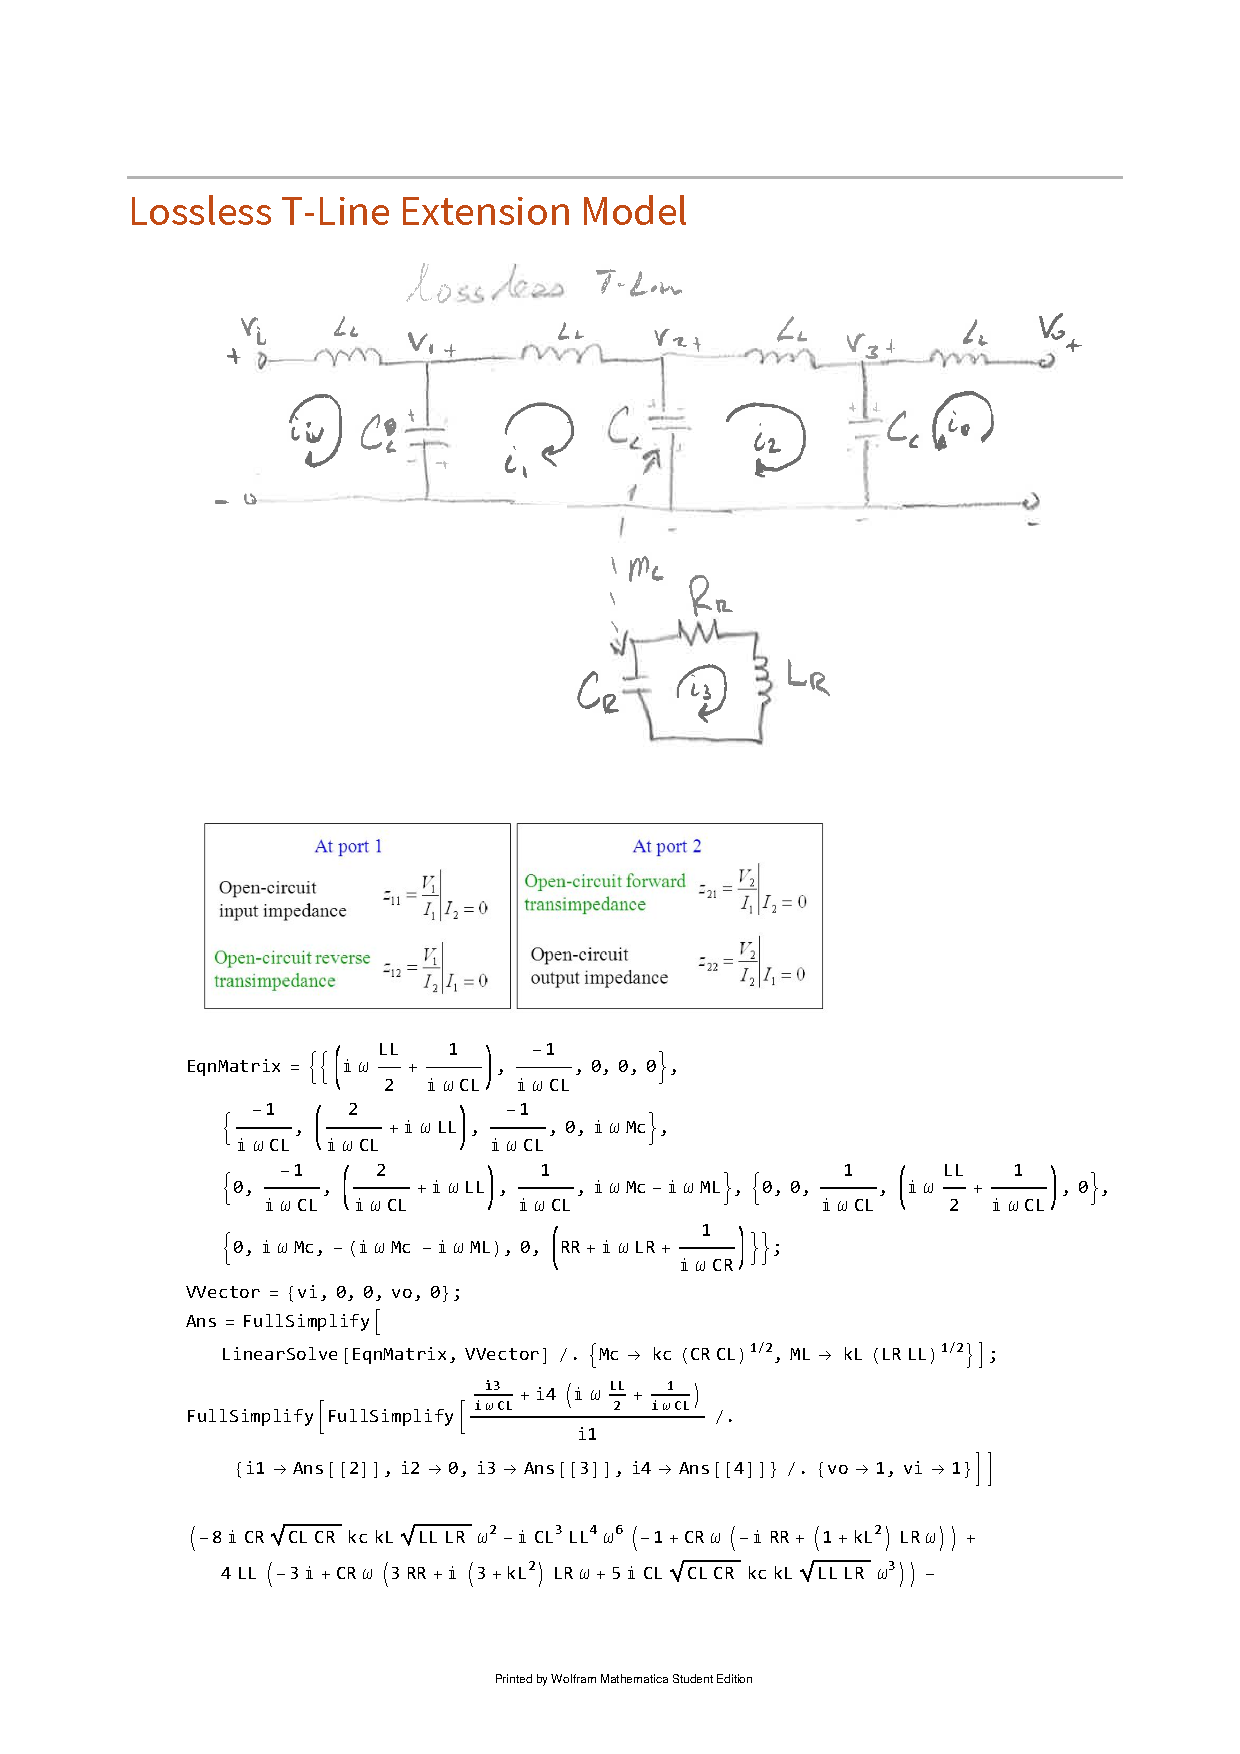
\includepdf[pages=-]{Kapitel/Appendix/MathematicaTHzWave.pdf}
\chapter[MatLab Code]{MatLab Code}
 	\definecolor{light-gray}{gray}{0.90}
\lstset{language=Matlab,%
    %basicstyle=\color{red},
    breaklines=true,%
    morekeywords={matlab2tikz},
    keywordstyle=\color{blue},%
    morekeywords=[2]{1}, keywordstyle=[2]{\color{black}},
    identifierstyle=\color{black},%
    stringstyle=\color{mylilas},
    commentstyle=\color{mygreen},%
    showstringspaces=false,%without this there will be a symbol in the places where there is a space
    numbers=left,%
    tabsize=2,
    frame=single,
    backgroundcolor = \color{light-gray},
    rulecolor=\color{black},
    numberstyle={\tiny \color{black}},% size of the numbers
    numbersep=9pt, % this defines how far the numbers are from the text
    emph=[1]{for,end,break},emphstyle=[1]\color{red}, %some words to emphasise
    %emph=[2]{word1,word2}, emphstyle=[2]{style},    
}

\section*{Generate setup for {\em esfit} minimization}
\lstinputlisting{Kapitel/Appendix/RegCrystal.m}
\newpage

\section*{Custom function for {\em esfit} minimization}
\lstinputlisting{Kapitel/Appendix/findangles.m}
\newpage


\section*{Generate the Resonance Roadmap using BestVals from {\em esfit}}
\lstinputlisting{Kapitel/Appendix/ResonanceRoadmap.m}

%\chapter[ESEEM Data of Hox from CpI.]{$^{14}$N Three-Pulse ESEEM Data of H$_{ox}$ from CpI.}

The following three-pulse ESEEM data was taken by following the fusca-colored resonance roadmap of Fig.~\ref{fig:xTalFeFe}A in Chapter 6. Herein, the $\tau$ starts at 200~ns, $t_1$ starts at 300~ns with 256 24~ns steps, and $\pi$-pulse is 80~ns at a microwave power of 7~mW. A total of 16 $\tau$ values are taken from 200~ns to 424~ns over an 18 minute collection time per trace.

\begin{figure}[ht]
 \centering
 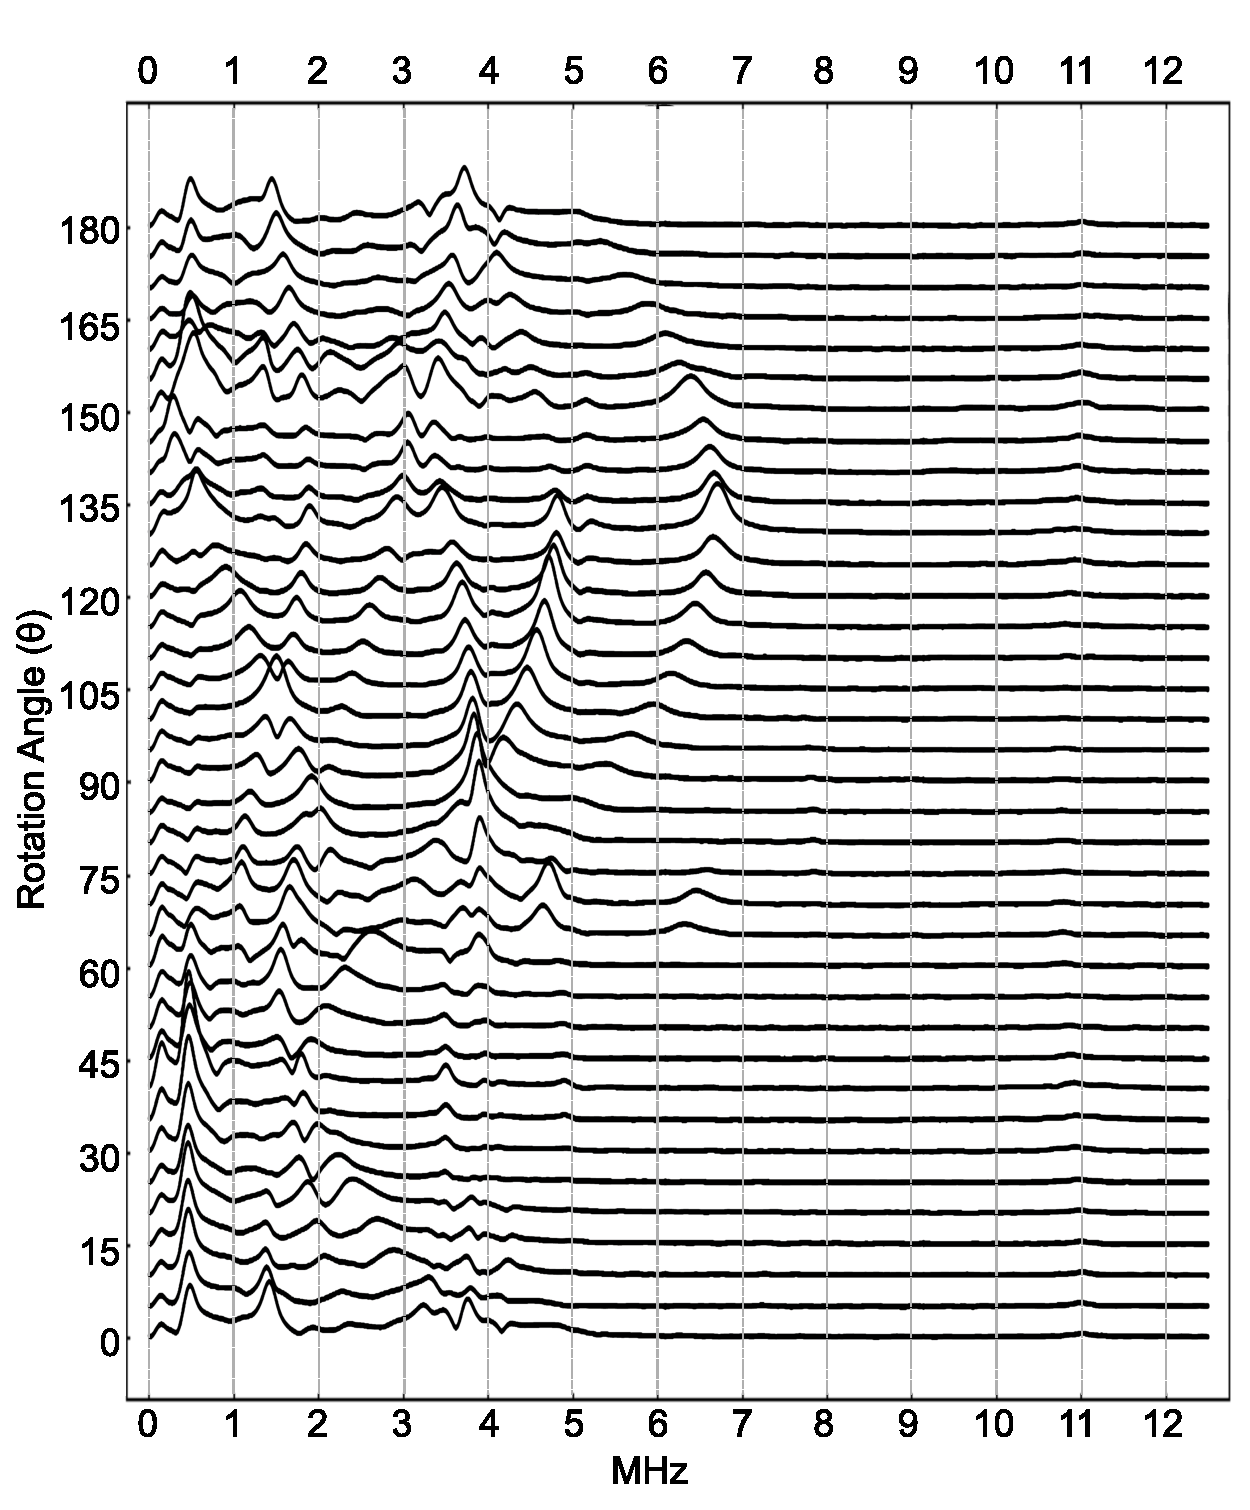
\includegraphics[width=0.85\textwidth]{Kapitel/Appendix/ESEEMFirstPeakA.eps}
 \caption[Preliminary Three-Pulse ESEEM Data of Hox]{Three-pulse ESEEM data from CpI in the H$_{ox}$ stable intermediate.}
 \label{fig-E:ESEEM}
\end{figure}

The data in Fig.~\ref{fig-E:ESEEM} represents the state-of-the-art signal-to-noise ratio for the study of protein single-crystals with volumes less than 3~nl. Further analysis is underway.


\end{appendices}

%%%%%%%%%%%%%%%%%%%%%%%%%%%%%%%%%%%%%%%%%%%%%%%%%%%%%%%%%%%%%%%%%%%%%%%%
%						Literaturverzeichnis
%%%%%%%%%%%%%%%%%%%%%%%%%%%%%%%%%%%%%%%%%%%%%%%%%%%%%%%%%%%%%%%%%%%%%%%%
\backmatter
\pagenumbering{Roman}
%\setcounter{page}{\theSeitenzahl}
%\addcontentsline{toc}{chapter}{\bibname}%je nach Klasse evtl. 'section' durch 'chapter' ersetzten
%\sloppy
%\printbibliography


%%%%%%%%%%%%%%%%%%%%%%%%%%%%%%%%%%%%%%%%%%%%%%%%%%%%%%%%%%%%%%%%%%%%%%%%
%							Anhang
%%%%%%%%%%%%%%%%%%%%%%%%%%%%%%%%%%%%%%%%%%%%%%%%%%%%%%%%%%%%%%%%%%%%%%%%
%\begin{appendices}
%	\include{Kapitel/Anhang}
%	\include{Kapitel/Anhang2}
%\end{appendices}

%%%%%%%%%%%%%%%%%%%%%%%%%%%%%%%%%%%%%%%%%%%%%%%%%%%%%%%%%%%%%%%%%%%%%%%%
%							Glossary
%%%%%%%%%%%%%%%%%%%%%%%%%%%%%%%%%%%%%%%%%%%%%%%%%%%%%%%%%%%%%%%%%%%%%%%%
%\printglossary[style=index]
%\printglossary[type=\acronymtype,style=index]
%\printglossary[type=symbols,style=index]
%\printindex
	
\end{document}